\documentclass[11pt, a4paper,oneside,chapterprefix=false]{scrbook}
\usepackage[T1]{fontenc}
\usepackage[font={small}]{caption}
\usepackage{a4wide}
\usepackage{times}
\usepackage{helvet}   % sets sans serif font

\usepackage{amsmath,amssymb,amsthm}

\usepackage{graphicx}
\usepackage{subfigure}  
\usepackage{fancybox} % for shadowed or double bordered boxes
\usepackage{fancyhdr}
\usepackage[dvipsnames]{xcolor}
\usepackage{rotating}

\usepackage{hyperref}
\hypersetup{
    colorlinks=true,
    linkcolor=blue,
    filecolor=magenta,      
    urlcolor=cyan,
}

\DeclareGraphicsExtensions{.pdf, .jpg, .png}
\DeclareOldFontCommand{\sf}{\normalfont\sffamily}{\mathsf}

%% macros
 \def\mathbi#1{\textbf{\em #1}}
 
% commands
\newcommand{\Adjoint}{\mbox{\rm Adj}}
\newcommand{\Area}{\mbox{\rm Area}}
\newcommand{\ACos}{{\mbox{\rm Cos}^{-1}}}
\newcommand{\ASin}{{\mbox{\rm Sin}^{-1}}}
\newcommand{\ATan}{{\mbox{\rm atan2}}}
\newcommand{\Code}[1]{{\tt #1}}
\newcommand{\Complex}{\mbox{\bf C}}
\newcommand{\Cross}{{\mbox{\rm Cross}}}
\newcommand{\Mydddot}[1]{\mbox{\shortstack{$.$\hspace*{-1pt}$.$\hspace*{-1pt}$.$\\$#1$}}}
\newcommand{\Degree}{\mbox{\rm degree}}
\newcommand{\Diag}{\mbox{\rm Diag}}
\newcommand{\Dim}{\mbox{\rm dim}}
\newcommand{\Dist}{\mbox{\rm Distance}}
\newcommand{\IntTwo}{\int\!\!\int}
\newcommand{\IntThree}{\int\!\!\int\! \!\int}
\newcommand{\Kernel}{\mbox{\rm kernel}}
\newcommand{\Kross}{\mbox{\rm Kross}}
\newcommand{\Grad}{\nabla}
\newcommand{\Perp}{\mbox{\rm Perp}}
\newcommand{\Point}[1]{{\cal #1}}
\newcommand{\Rank}{\mbox{\rm rank}}
\newcommand{\Range}{\mbox{\rm range}}
\newcommand{\Real}{{\mbox{\rm I}\hspace*{-2pt}\mbox{\rm R}}}
\newcommand{\RealSbt}{{\mbox{\rm\scriptsize I}\hspace*{-2pt}\mbox{\rm\scriptsize R}}}
\newcommand{\Res}{\mbox{\rm resultant}}
\newcommand{\Sbt}[1]{{\mbox{\rm\scriptsize #1}}}
\newcommand{\MySign}{\mbox{\rm Sign}}
\newcommand{\SignSBT}{\mbox{\rm\scriptsize Sign}}
\newcommand{\Skew}{\mbox{\rm Skew}}
\newcommand{\Span}{\mbox{\rm Span}}
\newcommand{\SqrDist}{\mbox{\rm Distance$^2$}}
\newcommand{\Trace}{\mbox{\rm Trace}}
\newcommand{\TRN}{{\mbox{\rm\scriptsize T}}}
\newcommand{\Vector}[1]{\mbox{\bf #1}}
\newcommand{\VectorM}[1]{\mbox{\boldmath $#1$}}
\newcommand{\Volume}{\mbox{\rm Volume}}

\newcommand{\IVec}{\mbox{\boldmath $\imath$}}
\newcommand{\JVec}{\mbox{\boldmath $\jmath$}}
\newcommand{\KVec}{\mbox{\boldmath $k$}}
\newcommand{\LVec}{\mbox{\boldmath $\ell$}}
\newcommand{\RMat}{{\cal R}}
\newcommand{\QMat}{{\cal Q}}
\newcommand{\QCMat}{\overline{\cal Q}}

\newcommand{\Lerp}{\mbox{\rm lerp}}
\newcommand{\Slerp}{\mbox{\rm slerp}}
\newcommand{\Quad}{\mbox{\rm quad}}
\newcommand{\Squad}{\mbox{\rm squad}}

\newcommand{\ODer}[2]{\frac{d #1}{d #2}}
\newcommand{\ODerT}[2]{\frac{d^2 #1}{d {#2}^2}}
\newcommand{\ODerM}[3]{\frac{d #1}{d #2 \, d #3}}
\newcommand{\PDer}[2]{\frac{\partial #1}{\partial #2}}
\newcommand{\PDerT}[2]{\frac{\partial^2 #1}{\partial {#2}^2}}
\newcommand{\PDerM}[3]{\frac{\partial^2 #1}{\partial #2 \, \partial #3}}

% mass density symbol
\newcommand{\Den}{\delta}

% environments
\newenvironment{BArray}[1]{\left\{ \begin{array}{#1}}{\end{array} \right\}}
\newenvironment{Combin}{\left( \begin{array}{c}}{\end{array} \right)}
\newenvironment{Matrix}[1]{\left[ \begin{array}{#1}}{\end{array} \right]}


\let\mbf=\mathbf
\let\mvec=\mathbf
\let\mcal=\mathcal
\let\mfunc=\mathrm

%\def\R{\mbox{\ensuremath{\mathrm{I\!R}}}}
\newcommand{\R}{\ensuremath{\mathbb{R}}}
\newcommand{\N}{\ensuremath{\mathbb{N}}}
\newcommand{\Z}{\ensuremath{\mathbb{Z}}}
\newcommand{\C}{\ensuremath{\mathbb{C}}}

\newcommand{\of}[1]{\left( #1 \right)}
\newcommand{\abs}[1]{\left| #1 \right|}
\newcommand{\norm}[1]{\left\Vert {#1} \right\Vert}
\newcommand{\gradient}[1]{\nabla{\!}_{#1}{\,}}
\newcommand{\twovec}[2]{\left( #1 \atop #2 \right)}
\newcommand{\threevec}[3]{\left(\begin{array}{c}#1\\#2\\#3\end{array}\right)}
\newcommand{\fourvec}[4]{\left(\begin{array}{c}#1\\#2\\#3\\#4\end{array}\right)}

\newcommand{\refsec}[1]{Section~\ref{sec:#1}}
\newcommand{\reffig}[1]{Fig.~\ref{fig:#1}}
\newcommand{\reftab}[1]{Tab.~\ref{tab:#1}}
\newcommand{\refeq}[1]{Eq.~(\ref{eq:#1})}

%\newcommand{\R}{\hspace*{0.1ex}{\sf I} \hspace{-0.3ex}{\sf R}}

%6.5
\newcommand{\eps}{\mbox{$\epsilon$}}
\newcommand{\dmin}{\mbox{$d_{\min}$}}
\newcommand{\dmax}{\mbox{$d_{\max}$}}
\newcommand{\dminmax}{\mbox{$[\dmin,\dmax]$}}

%4.2:
\def\M{\mathcal{M}}
\def\n{\mathbi{n}}
\def\p{\mathbi{p}}
\def\q{\mathbi{q}}
\def\x{\mathbi{x}}
\def\tp{^{\mathsf{T}}}

\let\vec=\mathbi%
\let\mat=\mathbf%
\let\set= \mathcal%

% Taken from (and slightly modified): http://stackoverflow.com/questions/741985/latex-source-code-listing-like-in-professional-books

\usepackage{listings}
\usepackage{courier}
\usepackage{color}
\definecolor{lightgray}{gray}{0.9}
\definecolor{commentgreen}{rgb}{0.2,0.56,0.2}
 \lstset{
         basicstyle=\footnotesize\ttfamily, % Standardschrift
         numbers=left,               % Ort der Zeilennummern
         numberstyle=\tiny,          % Stil der Zeilennummern
         %stepnumber=2,               % Abstand zwischen den Zeilennummern
         numbersep=5pt,              % Abstand der Nummern zum Text
         tabsize=2,                  % Groesse von Tabs
         extendedchars=true,         %
         breaklines=true,            % Zeilen werden Umgebrochen
         keywordstyle=\color{red},
                frame=b,         
          keywordstyle=[1]\textbf,    % Stil der Keywords
         keywordstyle=[2]\textbf,    %
         keywordstyle=[3]\textbf,    %
         keywordstyle=[4]\textbf,   %\sqrt{\sqrt{}} %
         stringstyle=\color{blue}\ttfamily, % Farbe der String
         showspaces=false,           % Leerzeichen anzeigen ?
         showtabs=false,             % Tabs anzeigen ?
         xleftmargin=17pt,
         framexleftmargin=17pt,
         framexrightmargin=5pt,
         framexbottommargin=4pt,
         backgroundcolor=\color{lightgray},
         showstringspaces=false,      % Leerzeichen in Strings anzeigen ?
         commentstyle=\color{commentgreen}
 }
 \lstloadlanguages{% Check Dokumentation for further languages ...
         %[Visual]Basic
         %Pascal
         %C
		PHP, 
         C++
         %XML
         %HTML
         %Java
 }
    %\DeclareCaptionFont{blue}{\color{blue}} 

  %\captionsetup[lstlisting]{singlelinecheck=false, labelfont={blue}, textfont={blue}}
  \usepackage{caption}
\DeclareCaptionFont{white}{\color{white}}
\DeclareCaptionFormat{listing}{\colorbox[cmyk]{0.43, 0.35, 0.35,0.01}{\parbox{\textwidth}{\hspace{15pt}#1#2#3}}}
\captionsetup[lstlisting]{format=listing,labelfont=white,textfont=white, singlelinecheck=false, margin=0pt, font={bf,footnotesize}}

\usepackage{color}
\definecolor{RED}{rgb}{1,0,0}
\definecolor{GREEN}{rgb}{0,0.7,0}
\definecolor{BLUE}{rgb}{0,0,1}
\newcommand{\FIXME}[1]{{\color{RED}{\textbf{FIX}: #1}}}

\addtolength{\textheight}{2.0cm}
\addtolength{\voffset}{-1cm}
\addtolength{\textwidth}{1.8cm}
\addtolength{\hoffset}{-.9cm}

\widowpenalty=10000
\clubpenalty=10000

\newcommand{\todo}[1]{}
\renewcommand{\todo}[1]{{\color{red} TODO: {#1}}}


\lstdefinelanguage{JavaScript2}{
  keywords={typeof, new, true, false, catch, function, return, null, catch, switch, var, if, in, while, do, else, case, break, for, forEach},
  keywordstyle=\color{orange}\bfseries,
  ndkeywords={class, export, boolean, throw, implements, import, this},
  ndkeywordstyle=\color{darkgray}\bfseries,
  identifierstyle=\color{black},
  sensitive=false,
  comment=[l]{//},
  morecomment=[s]{/*}{*/},
  commentstyle=\color{purple}\ttfamily,
  stringstyle=\color{ForestGreen}\ttfamily,
  morestring=[b]',
  morestring=[b]"
}

\begin{document}

\frontmatter
%\maketitle %automatic version
% --- selfmade version ----
\begin{titlepage}
	\setlength{\parindent}{0cm}
	\addtolength{\textheight}{1.0cm}

	\vspace{0.5cm}
	\Huge
	{\textbf{A visualization of biodiversity through time\\ }}

	\vfill \vfill \vfill
	\begin{center}
	\includegraphics*[width=0.8\textwidth]{figures/cover/cover}
    \end{center}
	\vfill
	\sf \Large
	Master Thesis \\
	January 31, 2022 \\[0.5cm]
	\large
	by Wuxing Dong, 18-946-038

	\vfill \vfill \vfill
	\begin{minipage}[b]{0.5\textwidth}
	Supervisors: \\
	Prof. Dr. Renato Pajarola \\
	Gaudenz Halter \\
	\end{minipage}
	%
	\begin{minipage}[b]{0.5\textwidth} \raggedleft
	Visualization and MultiMedia Lab \\
	Department of Informatics \\
	University of Z{\"u}rich
	\end{minipage}

	\vfill
	\hrule
	\vspace{0.5cm}
	\includegraphics*[width=0.3\textwidth]{figures/cover/uzh_logo} \hfill
	\includegraphics*[width=0.3\textwidth]{figures/cover/vmml_logo}
\end{titlepage}
%%

%=====================================================================

%=====================================================================
\chapter{Abstract} \label{chp:abstract}
%=====================================================================

The increasing size and dimensionality of datasets in the humanities pose new challenges to scholars working with them, including how to establish an overview over the dataset, how to establish new hypotheses and how to test them. Material, pattern, and texture usage in moving image is an attractive example of such multi-dimensional datasets in film studies, as an almost infinite number of combinations thereof are possible.\\ 
This thesis proposes interactive data visualization and exploration of film features as a solution to assist film researchers in the investigation of relationships between material, pattern, textures, and a wide range of qualitative analysis labels in a large film database. Using an array of visual components in combination with exhaustive computational methods and an interactive user-interface, the proposed solutions show to be effective in conveying the global and local structure of the dataset as well as the relationship between different feature groups of features. Finally, the resulting visualization tool is embedded into the well-established research framework of the FilmColors project.


%=====================================================================

\tableofcontents

\mainmatter


%=====================================================================
\chapter{Introduction} \label{chp:introduction}
%=====================================================================

\section{Effective visualization of data} \label{sec:one}
In the information age, the Internet has become a primary source to inform ourselves about the world. It is therefore a great opportunity for the scientific community to take advantage of the web and create high quality products to communicate their findings and ideas to the general public. Textbook-styled verbal explanations can be rigorous, however, they easily become tedious and are already made available by school and college education. Videos are based on visual learning and are quick to absorb, yet there is little engagement with the viewers. Interactive data visualizations provide an excellent way for users to understand scientific concepts. New knowledge is conveyed by direct visual impact that easily draws attention, and insights can be formed by actively exploring the data and observing the response of the presentation due to the users' own actions. This learn-by-doing strategy is considered to be beneficial for consolidating new knowledge \cite{schank1995we}. \\

Although graphics play a major role to deliver scientific messages, there is a lack of formal theory on producing good graphics, and domain experts tend to rely on practical experiences that are guided by certain design principles \cite{chen2007handbook}. Increasing amount of studies have focused on concluding such principles \cite{senay1990rules,evergreen2013design,midway2020principles}. Chen and colleagues \cite{chen2007handbook} have summarized that three main aspects to pay attention to in a visualization project are its contents, the relevance in the context of the larger whole as well as the forms and aesthetics (the construction). Similarly, McCandless \cite{mccandless2014knowledge} argued that a good visualization requires the integrity of information, the interestingness of story (concept), the usefulness of goal and the beauty of the visual form.\\

Before embarking on producing a visualization, one should note the characteristics of human visual perception to improve the design strategies in practice. Cognitive psychology studies are aimed at examining human visual attention by exposing users to certain visual processing tasks. The results of those studies suggested some guidelines for more effective visualization. When the visual features of a certain type of data is expected or previously known, the accuracy and speed of visual perception is drastically improved \cite{haroz2012capacity}. Therefore, the authors suggested that a visual feature should be assigned to the same data dimension, or type of data \cite{haroz2012capacity}. It is also important to note that attention is limited and selective, therefore the amount and diversity of information should be kept within the limits of cognitive load \cite{alhadad2018visualizing}. When many categories of data are present, compromises are needed to retain graphics complexity and only demonstrate a few categories at a time. \\

Through early years of research on how images are analyzed visually, it has been found that detailed vision is only achievable by actively focusing on a small portion of the visual field \cite{itti2001computational, noton1971scanpaths}. However, a few visual features, such as colors and curvatures, are subjected to pre-attentive processing, which can be effortlessly and rapidly detected by low-level visual processes \cite{healey2011attention}. Therefore, the appropriate use of limited but distinctive colors and simple shapes is a powerful technique. They are also the leading factors to make a visualization memorable \cite{borkin2013makes}. \\

With respect to the design process, it should be guided by the core messages to deliver. It is important to first prioritize what information to show, envision the final result, and then choose appropriate colors and geometries that fulfill the objectives \cite{midway2020principles}. The most efficient geometry should be of high data-ink ratio, which is the ratio between the amount of ink allocated on the actual data to the total amount of ink a figure consumes \cite{tufte1983visual}. While striving for a high data-ink ratio, it is also important for a visualization to be simple, self-explanatory and straight to the point, such that the viewers are not overwhelmed with too much information. \\

The topic this thesis chooses to visualize is biodiversity through Earth history. There are biodiversity visualizations that are tree-based \cite{block2012deeptree}, map-based \cite{janicki2016visualizing}, or plot-based \cite{liang2019bioactivity}. However, there lacks a rich and interactive visualization on the Internet that illustrates biodiversity with both a dynamic tree of life and a map that locates species on the planet throughout millions of years. This thesis is intended to fill this gap. Furthermore, it is important to raise the awareness of the general public on ecological issues, in light of the current age of climate change. By exploring how different forms of life came to exist, thrive, and perish through a simple and interesting visualization, viewers could appreciate the inseparable relationship between life and its environment.

\section{Background on biodiversity and tectonic change} \label{sec: two}
Biodiversity is a result of evolution. Current views on species formation are based on modern evolution theory \cite{bowler1989evolution} originated from Darwin's work. To summarize briefly, all forms of life are argued to share a common ancestor, which diversified over the course of evolution to form the current tree of life. An organism's genetic information is encoded in DNA or RNA, which is replicated over generations. However, recombination and random mutation events occur during the replication process, resulting in genetic variations, which in turn cause the difference in phenotype, \emph{i.e.}, the observable traits of organisms. Individuals with traits that are more suitable to their particular environment are more likely to survive and pass their genes to their offspring, compared to those that are poorly adapted to the environment. This process is termed natural selection. Finally, a new species is formed during the process of speciation. It occurs when enough genetic variations are accumulated between the original population and the descendant population, such that organisms from the two groups are not capable of producing fertile offspring, namely, the two groups have formed reproductive isolation. A classic example of evolution is the adaptive radiation of finches on the Galapagos islands \cite{lack1983darwin}. The beak shapes of the finch species on different islands diversified to specialize in obtaining the dominant type of food on those islands.  \\

It is believed that life emerged from 3.5 billion years ago \cite{algeo1998terrestrial}. The past 540 million years (the Phanerozoic Eon) have seen rapid development and diversification of life. Throughout evolutionary history, there are records of drastic changes in biodiversity occurring in a relatively short period of time. On one hand, radiations are rapid increase in biodiversity. An example is the Cambrian explosion, during which most phyla of multi-cellular organisms originated \cite{alroy2001effects}. On the other hand, biodiversity experiences rapid declines during mass extinction periods. There is evidence of five mass extinction periods, one of which is the Cretaceous-Paleogene extinction event, when the dinosaurs were exterminated and mammals thrived due to their selective advantage given by their fur in the cooling environments \cite{courtillot2002evolutionary}. These periods of radiations or extinctions are caused by special events, plate motions, as well as changes in climate, such as temperature and oxygen level \cite{butterfield2009oxygen, svenning2007ice}. \\

Apart from biodiversity, the shape of the world also changes significantly throughout billions of years \cite{wilson1963continental}. Earth crust is composed of a number of tectonic plates undergoing constant motions. The heat generated from the interior of the planet causes the movement of the plates. Plate motion results in new landscapes and new continents, affecting lives inhabiting them. For instance, current continents are thought to belong to one supercontinent called Pangaea \cite{stampfli2013formation}, which gradually assembled approximately 335 million years ago (Paleozoic-Mesozoic) and drifted apart at around 175 million years ago (Triassic-Jurassic). \\

As the continents separate, populations from the same species are geographically isolated into their particular environments resulting from plate motion. Since organisms are under constant selective pressure, new species evolve in the newly created environments. Numerous studies support that tectonic movement plays an important role in driving biodiversity in various regions of the world. To list a few examples, Miocene tectonics contributed to the diversification of ungulate and carnivores in western United States \cite{kohn2008miocene}; the formation and break-up of Pangaea have driven global marine invertebrates diversity for the past 443 million years \cite{zaffos2017plate}, and the beginnings and movements of tropical reef biodiversity hotspots can be predicted by modeling plate motion for the past 140 million years \cite{leprieur2016plate}. 

\section{Aim of the thesis}
This thesis aims at building a web application that visualizes the change in biodiversity through the course of Earth history. In the final product, users can view a customizable tree of life during a selected time period under a selected taxonomy. In the meantime, the fossil records associated with the displayed tree of life are shown on a map of the selected time period. 

\section{Thesis structure}
Chapter \ref{chp:introduction} introduces the topic of data visualization and domain specific background information, and it claims the goal of the thesis. Chapter \ref{chp:related_work} analyzes some related work, indicating what could be learned and improved for the visualization to be built. Chapter \ref{chp:problem_statement} outlines the problems to be solved at each stage for building the web application. Chapter \ref{chp:technical_solution} discuses the technical solutions for solving the stated problems. Chapter \ref{chp:implementation} addresses how the technical solutions are implemented to result in the visualization product. Chapter \ref{chp:results} reports the result of the product. Chapter \ref{chp:conclusion} concludes the project and suggests future work.


%=====================================================================
\chapter{Related work} \label{chp:related_work}
%=====================================================================

There already exists an abundance of visualizations on the Internet regarding to tree of life as well as plate motion. This section discusses some selected works on these two topics. 

\section{Tree-based visualizations on biodiversity}
OneZoom (\url{https://www.onezoom.org/}, Figure \ref{fig:OneZoom}) visualizes all known living things in a fractal tree, and it is targeted for both professionals and the masses \cite{rosindell2012onezoom}. Users can zoom into or out of different levels of the tree by scrolling, and they can search for a particular node by its name. 

\begin{figure}[h]
	\centering
	\subfigure[The overview of OneZoom's tree from root. ]{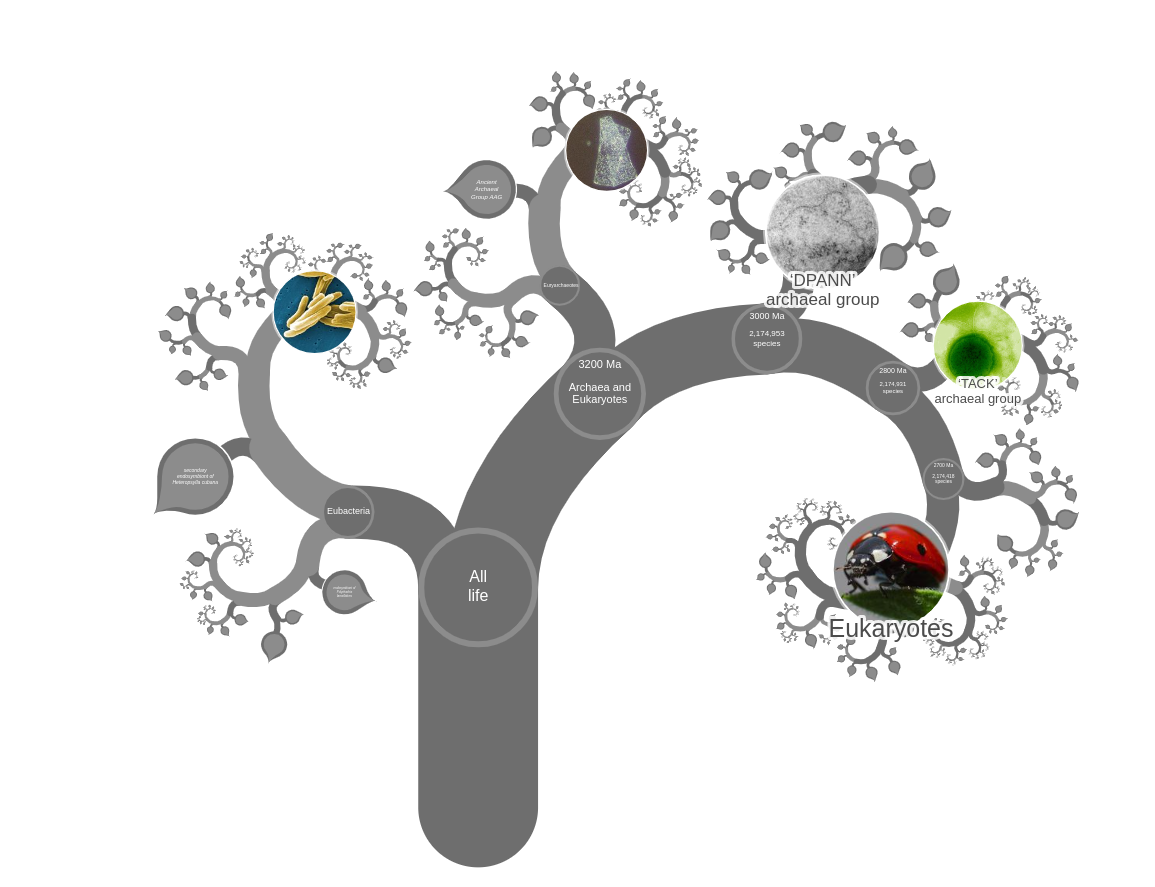
\includegraphics[width=0.45\textwidth]{figures/related_work/onezoom_overview}\label{fig:OneZoom_a}} 
	\hfill
	\subfigure[The view on OneZoom's tree when zoomed onto mammals. ]{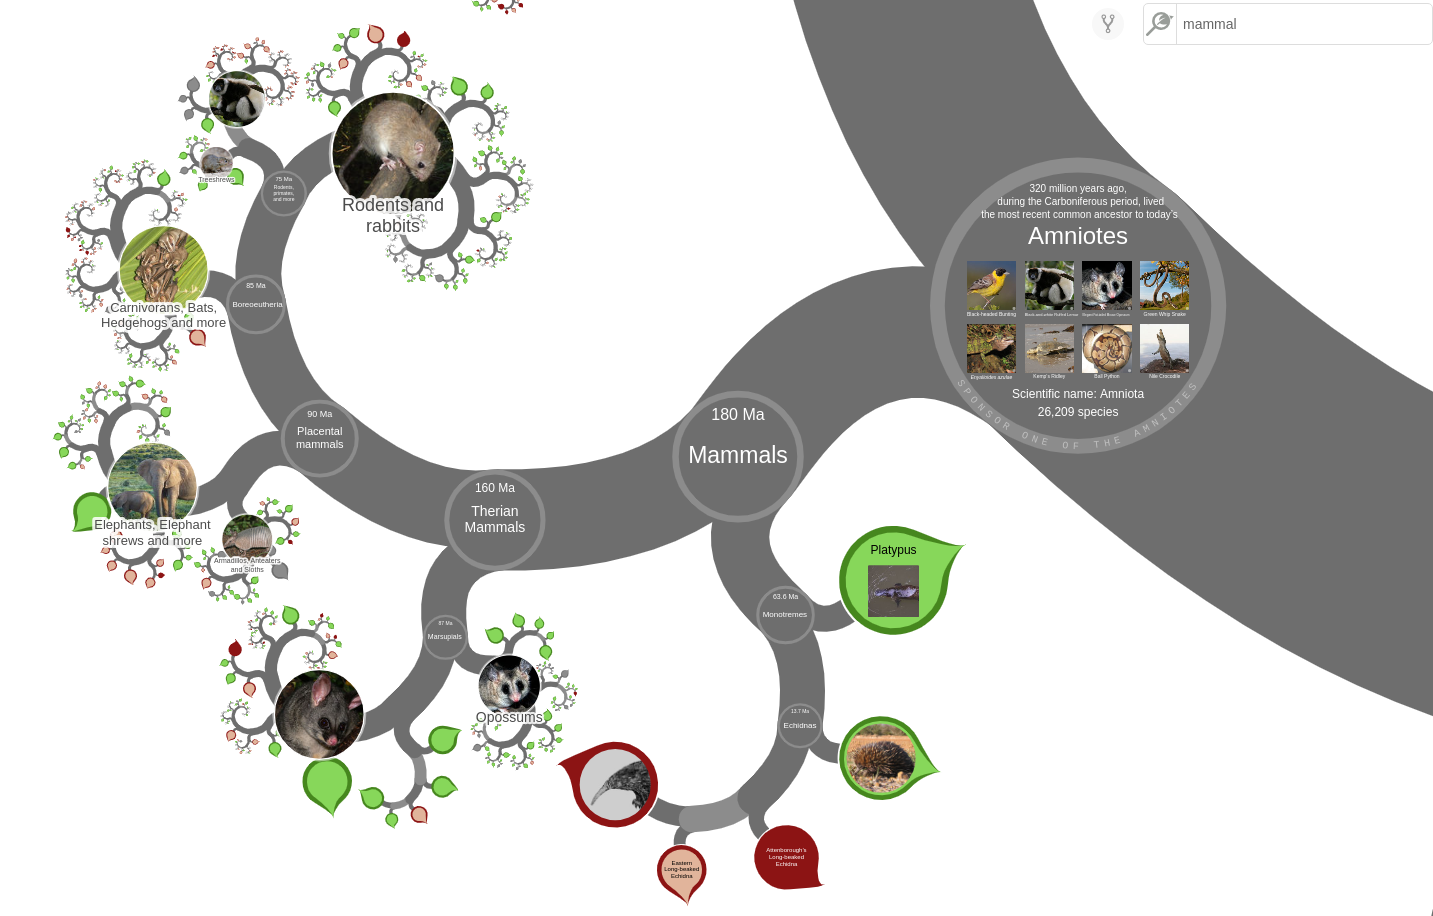
\includegraphics[width=0.45\textwidth]{figures/related_work/onezoom_mammal}\label{fig:OneZoom_b}} 
	\caption{Tree of life implementation in OneZoom. }
	\label{fig:OneZoom}
\end{figure}

The fractal design gives the tree a nice appearance, with a high resemblance to an actual tree. Information such as images or the earliest time of a node is also well packed in the interactive image. There is a reset button to return to the root and a drop-down list that provides links to the nodes along the path from the current position to root. These functions are convenient for navigation and similar functionality should be implemented in this thesis. It is claimed that all categorized organisms, with a total amount of over two million, are included in the tree. Each species in the tree is incorporated with a phylogenetic classification. This leads to the fact that when users attempt to visit the root from a given species on a leaf node, they visit all of the nodes representing each of its ancestors throughout evolutionary history. Although how a certain organism evolved from the common ancestor of all life can be rigorously inspected, from the user experience's point of view, the tree is extremely deep. Apart from manually searching for a name, navigating to the desired location in this deep tree is mainly achieved by scrolling and dragging the item of interest to the center of the screen. This makes it difficult for viewers to relocate to a different section of the tree, or to gain an overview of where the current node positions in the entire tree of life. To reach the root of all life (Figure \ref{fig:OneZoom_a}) from the mammal (Figure \ref{fig:OneZoom_b}), users need to scroll through all upper layers of the tree, which have a similar-looking spiral structure that appears to be confusing and disorienting. A similar tree of life visualization is Lifemap (\url{http://lifemap.univ-lyon1.fr/explore.html}, \cite{de2016lifemap}), which ameliorates the navigation difficulty by highlighting the ancestry path from root to a node (Figure \ref{fig:lifemap}). However, due to the sheer depth of the tree, users still need to travel deep into the tree by scrolling. Rather than demonstrating the exact ancestral paths, the purpose of the tree for this project is to organize each species such that biodiversity can be viewed in an intuitive way. As a consequence, all nodes can be organized by the main standard taxonomic ranks, in the descending order of domain, kingdom, phylum, class, order, family, genus , and species. This limits the tree's depth to be eight and thus simplifies the navigation process. In addition, to avoid scrolling and dragging, the tree can take a fixed position. Users can select a node of interest as a root, and only the subtree that is rooted by the chosen node is shown. In the meantime, the location of the selected node in relation to the complete tree of life can be shown in a clickable breadcrumb structure that 1, provides an overview of the whole tree by demonstrating the path from the root of all life to the current root and 2, allows users to easily navigate to any of the upstream nodes in the tree by clicking. \\

\begin{figure}[h]
	\centering
	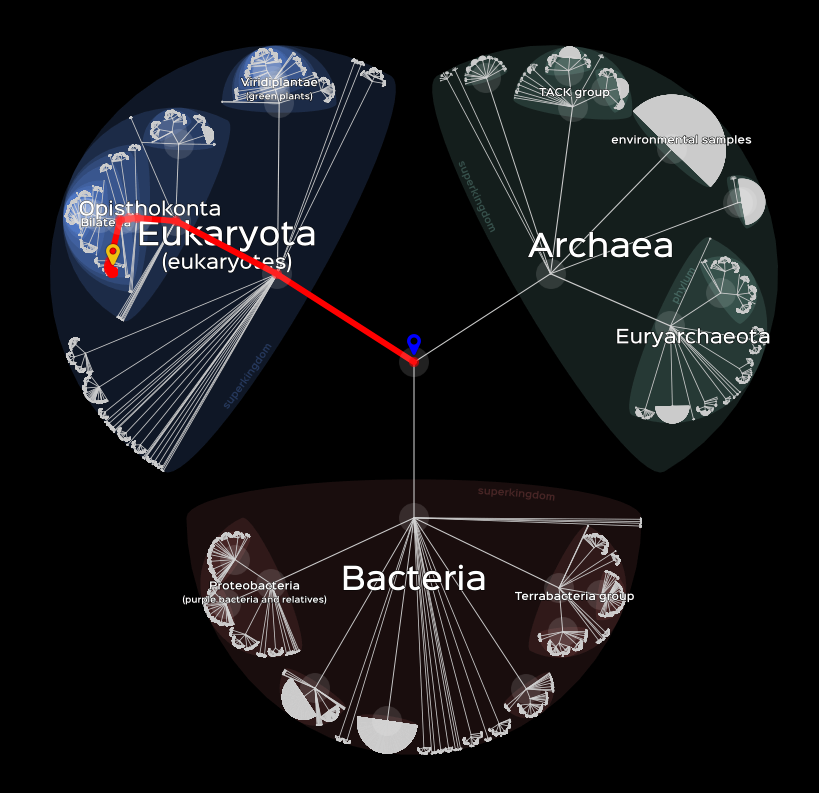
\includegraphics[width=0.5\textwidth]{figures/related_work/lifemap}
	\caption{Lifemap enables a "path from root" functionality that highlights the ancestry path from \textit{Homo sapiens} to the root. Although due to its small size, the name \textit{Homo sapiens} is not longer visible.}
	\label{fig:lifemap}
\end{figure}

A much more simplified version of the tree of life is Evogeneao (\url{https://www.evogeneao.com/en/explore/tree-of-life-explorer}, no publication), which is intended for school education. As shown in Figure \ref{fig:evogeneao}, all species are clustered into clearly colored regions, giving the viewers a direct and memorable visual impact. A similar coloring and grouping design could be adapted in this project. With the tree of life arranged in a half-circle that is labeled with time and a few iconic events, users could get a view of how life radiated from the common ancestor into great diversity, and how this process is affected by special events on the planet. Since only a small subset of all organisms are shown, the tree is small and can be entirely shown, therefore always giving the audience an overview. However, this web application provides the little possibility of exploration due to its limited options for interaction, as the main functionality is to show the common ancestor of two selected items (Figure \ref{fig:evogeneao_b}).\\

\begin{figure}[h]
	\centering
	\subfigure[The overview of Evogeneao's tree. ]{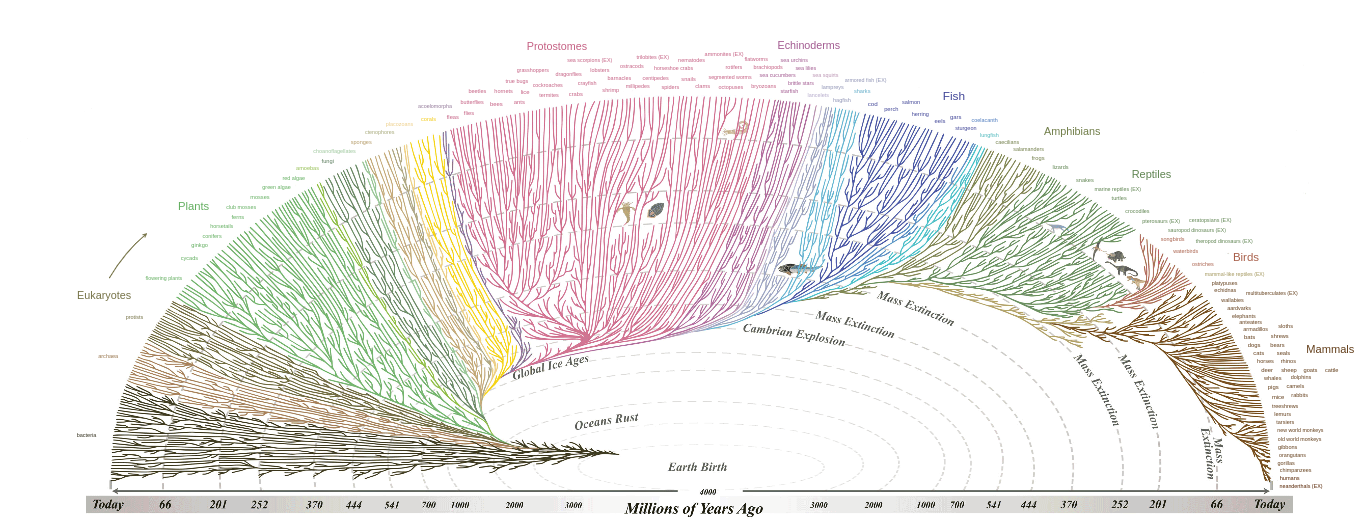
\includegraphics[width=0.45\textwidth]{figures/related_work/evogeneao_overview}\label{fig:evogeneao_a}} 
	\hfill
	\subfigure[The ancestral relationship between human and songbird. ]{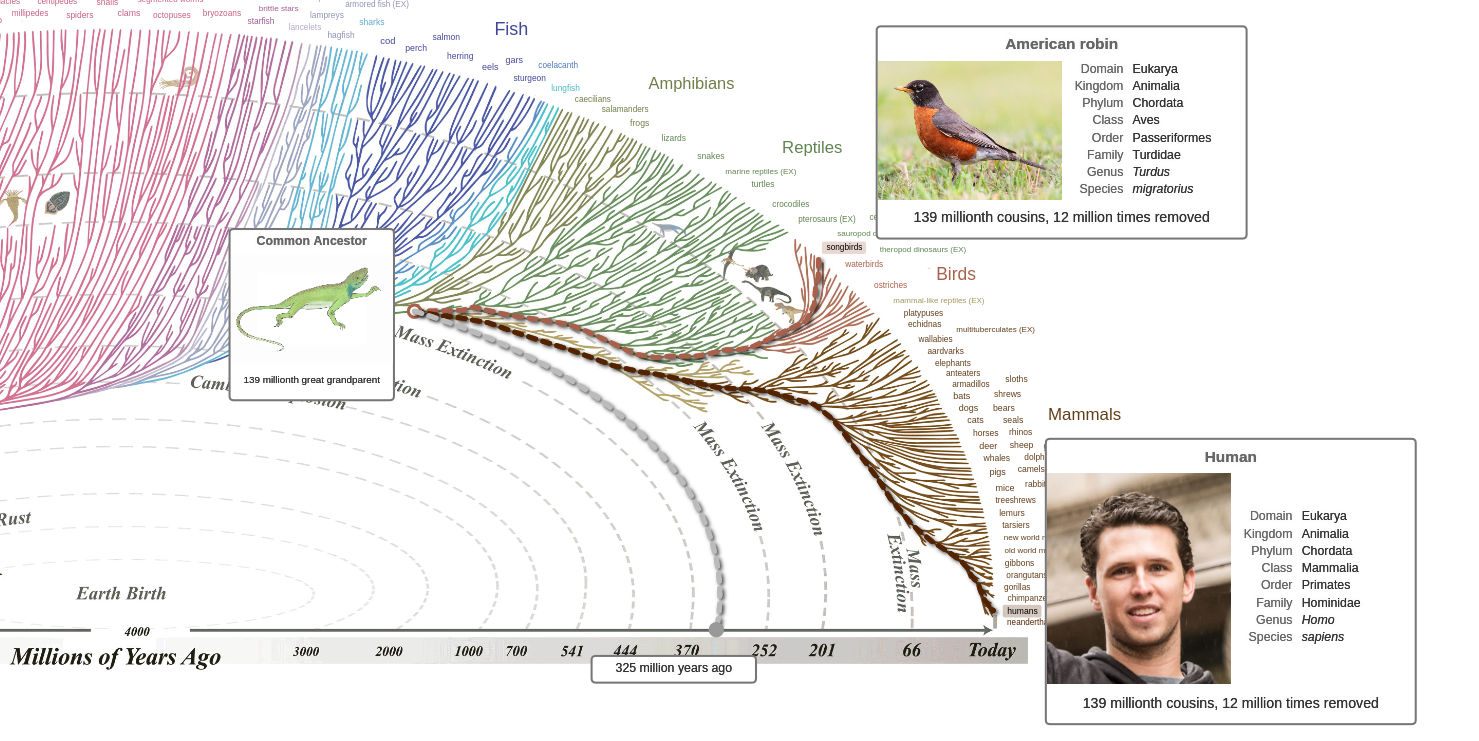
\includegraphics[width=0.45\textwidth]{figures/related_work/evogeneao_relationship}\label{fig:evogeneao_b}} 
	\caption{Tree of life implementation in Evogeneao. }
	\label{fig:evogeneao}
\end{figure}

Finally, there are a wide variety of tree of life visualized for computational biologists, such as AnnoTree \cite{mendler2019annotree}, phylogeny.IO \cite{jovanovic2019interactive}, T-BAS \cite{carbone2017t} and PhyloWidget \cite{jordan2008phylowidget}, to list a few. These visualizations provide rich functionality for bioinformatic analysis that are well beyond the need of the general public and often make efforts to use. A typical example is iTOL (\url{https://itol.embl.de/itol.cgi}, Figure \ref{fig:iTOL}, \cite{letunic2019interactive}). The design of arranging all leaf nodes on the edge of a circle and all non-leaf nodes in its interior utilizes space effectively, therefore providing a good hint for our implementation.\\

\begin{figure}[h]
	\centering
	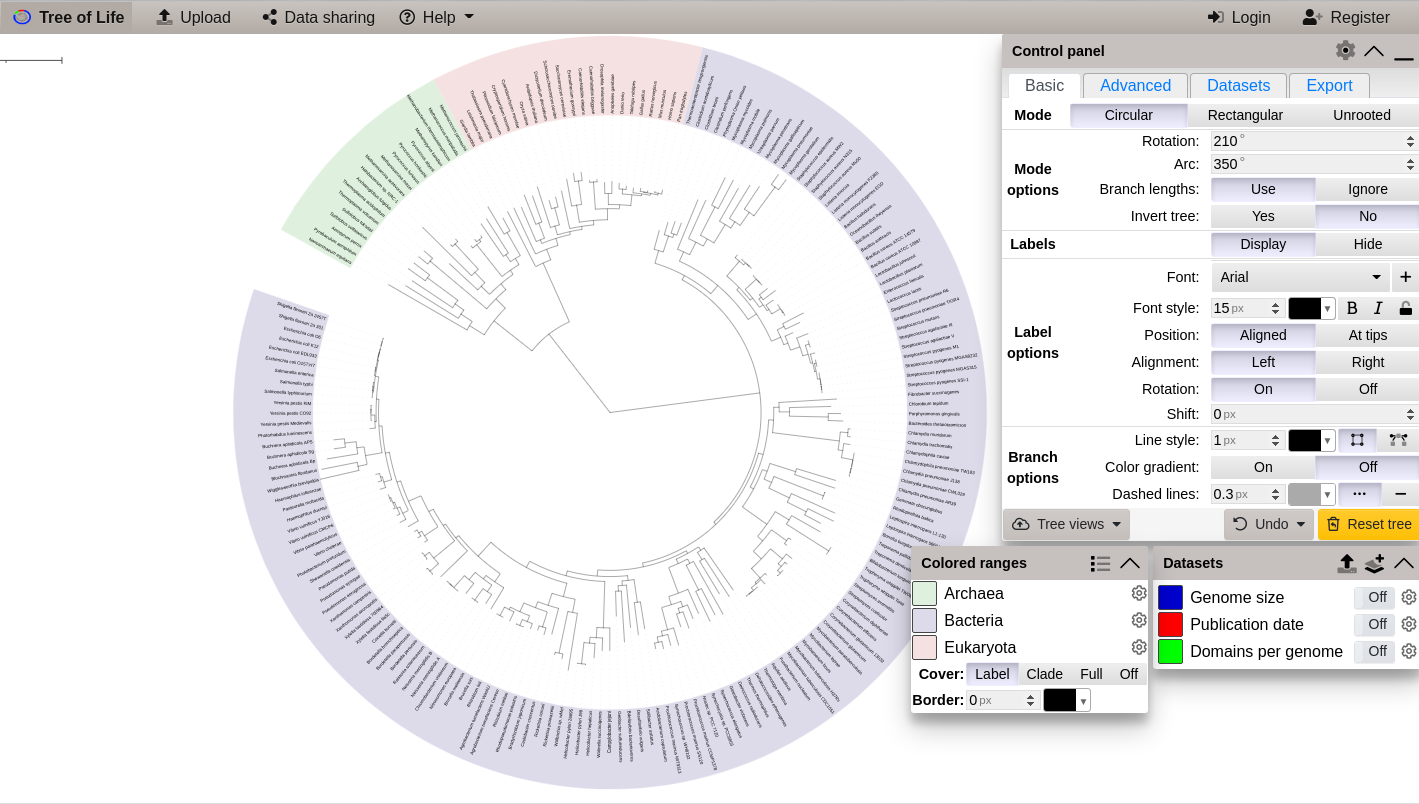
\includegraphics[width=0.5\textwidth]{figures/related_work/iTOL}
	\caption{Tree of life in iTOL. }
	\label{fig:iTOL}
\end{figure}

\newpage

\section{Visualizations on tectonic shift}
The current project involves visualizing paleogeography at various time points, since fossil points are displayed on a world map during the time period of interest. Rather than web-based, most visualizations on tectonic changes are commercial software products that are primarily intended for inspecting global petroleum and ore reserves.  Many products targeting the scientific community fall into the category of GIS software \cite{steiniger2010gis}. They are designed for analytic purposes. However, they are necessarily intuitive to operate or visually pleasing, such as GMAP \cite{torsvik1999plate}, PaleoMac \cite{cogne2003paleomac}, PLACA \cite{matias2005placa} and PPlates \cite{smith2007re}. \\

In more recent years, PaleoSim (Figure \ref{fig:paleoSim}, \cite{rogge2010visualization}) visualizes the ancient Earth by proposing a tectonic morphing model that simulates a smooth transformation of plates through time from image data. Users can select a time point or a particular plate and observe its shape throughout ancient history. However, this offers limited functionality, as it is not capable of tracking the location change of a given point on the map, which is needed for visualizing fossils. Nevertheless, GPlates (Figure \ref{fig:gplates}) is a next-generation software widely used for plate tectonics purposes \cite{boyden2011next} \cite{williams2012open} \cite{gurnis2012plate}. In short, the software receives a tectonic simulation model that defines how the movement of plates occurs through time, and vector data that represents geospatial information in points, lines, or polygons. It can then assign all geospatial data to a plate-tectonic reference, before reconstructing the geography at a requested time point and exporting the reconstruction into files. In relation to our project, it provides a method to trace a fossil point by assigning it to a certain plate, such that how its position alters can be calculated with a given tectonic model. As a result, this tool is used for our project, to reconstruct both the world map and the fossil points at a given ancient time point. \\

\newpage
\begin{figure}[h]
	\centering
	\subfigure[PaeloSim visualization on South America and Africa 105 million years ago. The figure is directly adopted from \cite{rogge2010visualization}. ]{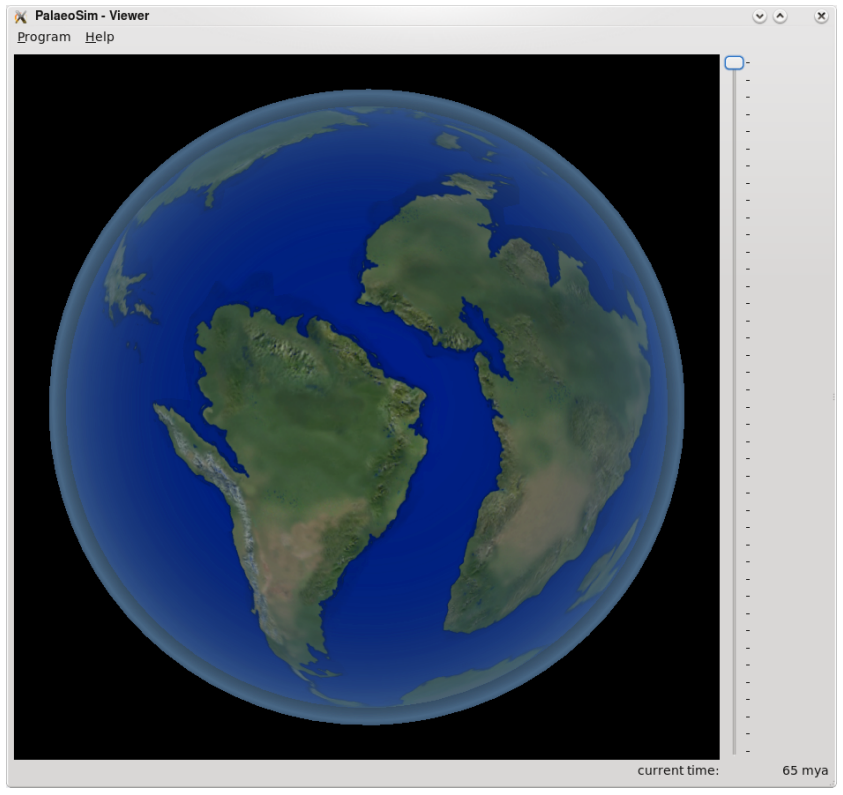
\includegraphics[width=0.45\textwidth]{figures/related_work/paleoSim}\label{fig:paleoSim}} 
	\hfill
	\subfigure[GPlates visualization of ancient earth at 710 million years ago, based on a model by \cite{li2008assembly}. The figure is directly adopted from \cite{williams2012open}. ]{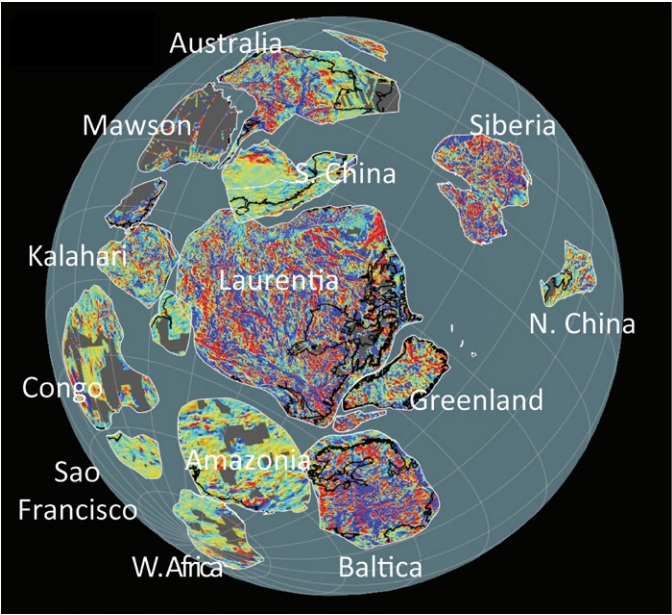
\includegraphics[width=0.45\textwidth]{figures/related_work/gplates}\label{fig:gplates}} 
	\caption{Example software-based visualizations on tectonic shift. }
	\label{fig:software_tectonic}
\end{figure}

A few web-based projects on continental drift visualization can also be found. Two typical products are Ancient Earth (\url{https://dinosaurpictures.org/ancient-earth#240}, Figure \ref{fig:ancient_earth}, no publication) and Earth Viewer (\url{https://www.biointeractive.org/classroom-resources/earthviewer}, Figure \ref{fig:earth_viewer}, no publication). Both of them show the coastlines of the continents at a select time point on a three-dimensional globe. Ancient Earth allows users to pick a particular time point from a list of options and search for the ancient location of a city. Earth Viewer provides more detailed information on geological time, and selectable time points are incremented every five million years on the scroll bar. Time periods are organized in a hierarchical structure, which can be adapted in this project for easy navigation. When clicking on a time period, instead of directing the user to view that time period, a pop-up window containing a brief introduction appears, which is counter-intuitive. An improvement is to show the Earth of the selected time period upon clicking. \\

\begin{figure}[h]
	\centering
	\subfigure[Tectonic shift visualized in Ancient Earth. ]{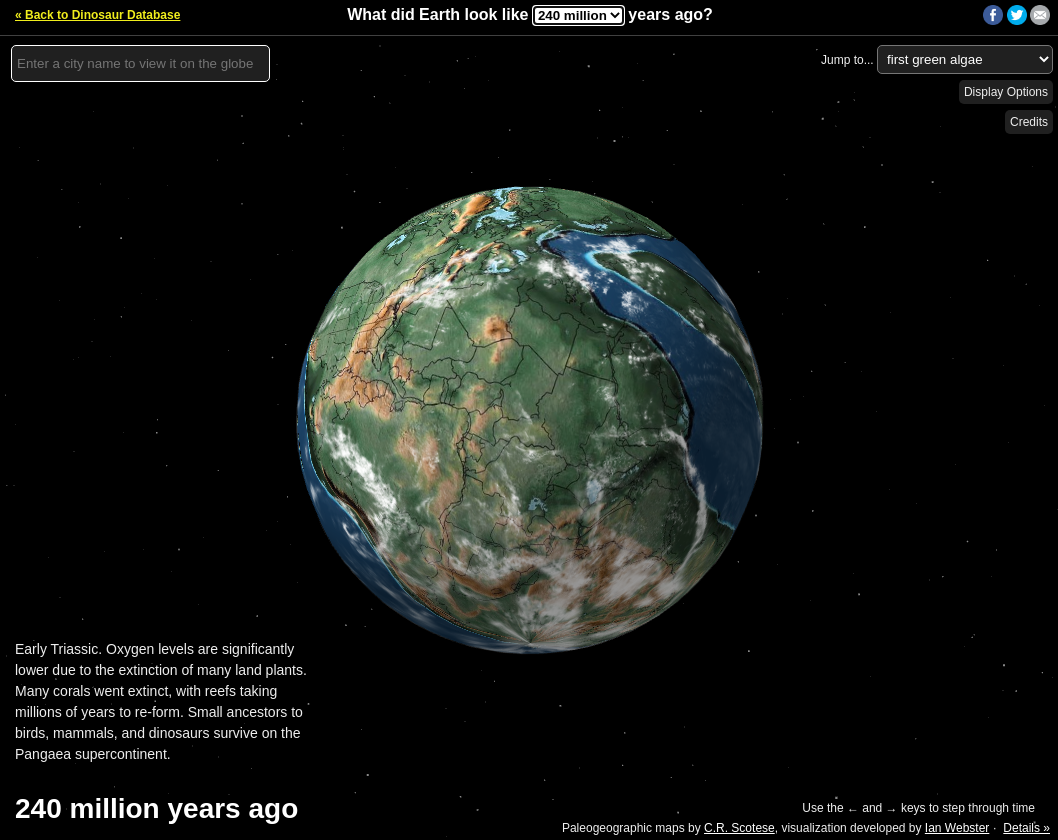
\includegraphics[width=0.45\textwidth]{figures/related_work/ancient_earth}\label{fig:ancient_earth}} 
	\hfill
	\subfigure[Tectonic shift visualized in Earth Viewer. ]{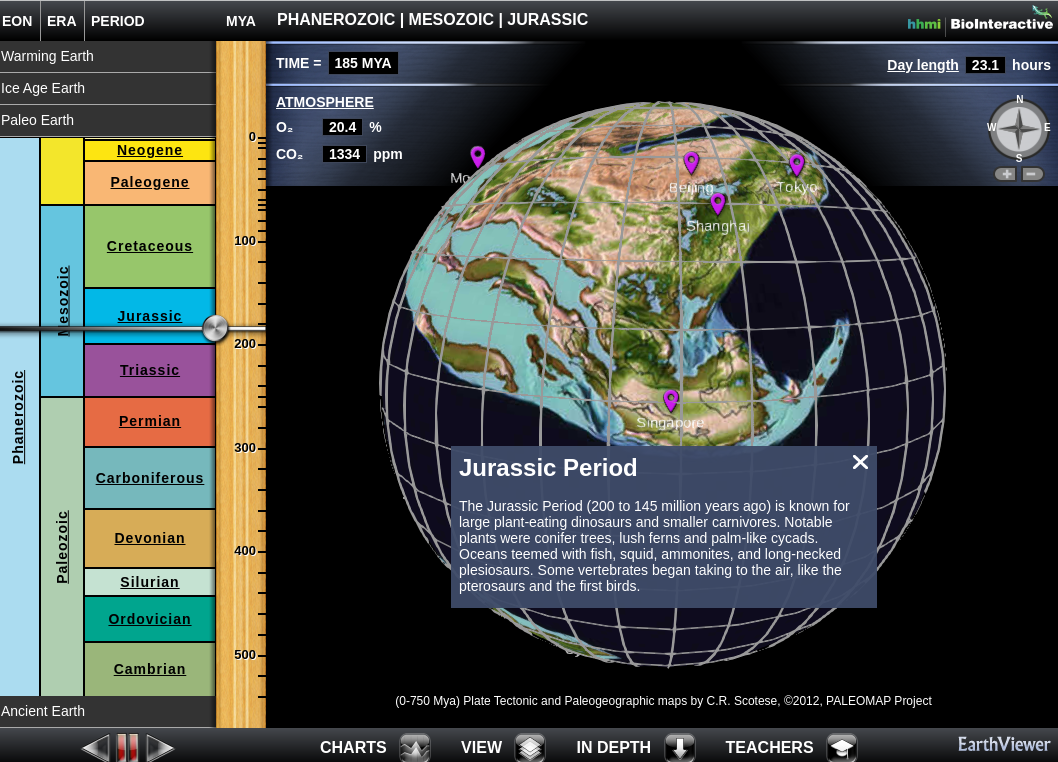
\includegraphics[width=0.5\textwidth]{figures/related_work/earth_viewer}\label{fig:earth_viewer}} 
	\caption{Example web-based visualizations on tectonic shift. }
	\label{fig:web_tectonic}
\end{figure}
%=====================================================================
\chapter{Problem statement} \label{chp:problem_statement}
%=====================================================================
The data visualization project is divided into several sub-problems as follows.

\begin{itemize}
	\item \textbf{Data processing}
	\begin{itemize}
		\item Process the PBDB dataset to extract fossil records 
		\item Extract a tree of life from the taxonomy information of the fossil records
		\item Trace the coordinates of each fossil record to ancient times
	\end{itemize} 
	\item \textbf{Database setup}: store the fossil data, coordinate data and the taxonomy data into a database
	\item \textbf{Back-end building}: provide a server for queries from the database upon front-end requests induced by users 
	\item \textbf{Front-end building}: visualize interactive components for users to explore biodiversity through deep time
	\begin{itemize}
		\item A time component that lists ancient time periods that users can select
		\item A tree component that shows the tree of life constructed by the fossil records found in the selected time period, under the selected taxonomy
		\item A map component that shows the shape of the continents in the selected time period, and the locations of the fossils that constitute the tree of life   
	\end{itemize} 
\end{itemize} 

%=====================================================================
\chapter{Technical solution} \label{chp:technical_solution}
%=====================================================================
\section{Overview}\label{sec:tec_overview}
This section explains the technical solutions to the problems stated in chapter \ref{chp:problem_statement}. To summarize, the project is divided into data processing in section \ref{sec:tec_data_processing}, database setup in section \ref{sec:tec_database_setup}, back-end query processing in section \ref{sec:tec_backend} and front-end development in section \ref{sec:tec_frontend}.

\begin{figure}[h]
	\centering
	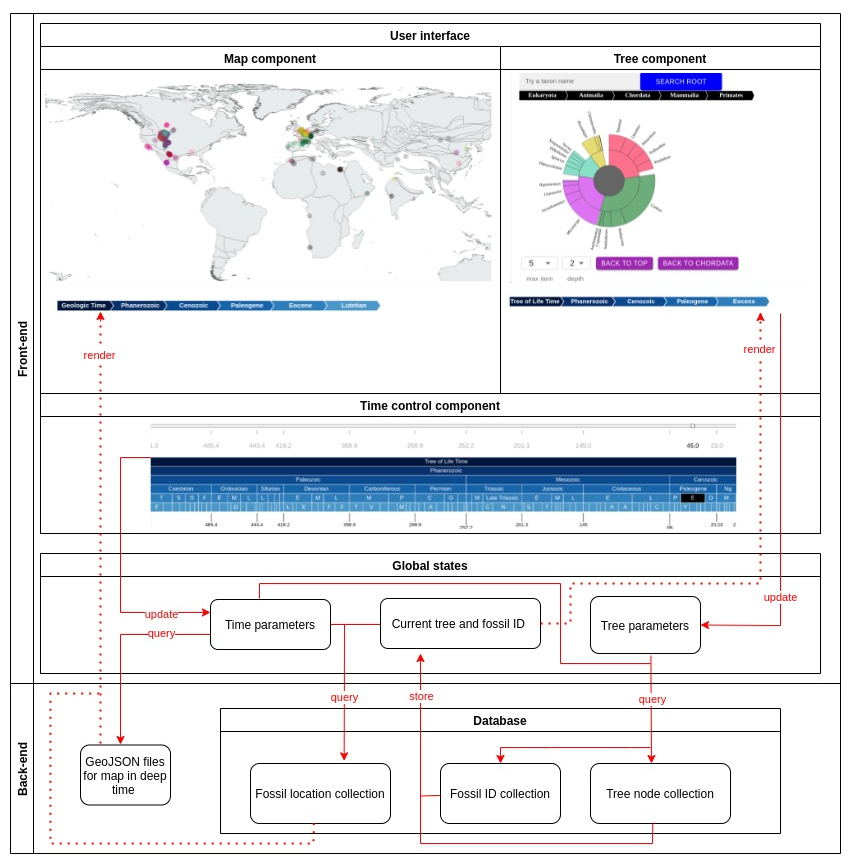
\includegraphics[width=0.9\textwidth]{figures/technical_solution/architecture}
	\caption{An overview of the architecture solution for the project. The user interface consists of a map, a tree, and a time control. The global states store tree and time parameters that are customized by users, and the current tree nodes attached with fossil ID sent from the database. The back-end resolves queries on the tree, fossil locations, and map, before sending results back to the front-end, where the data is visualized. }
	\label{fig:architecture}
\end{figure}

Diagram \ref{fig:architecture} proposes a structure of the designed visualization system. The front-end of the web application has a user interface and global states section that stores variables accessible to the components of the user interface. The back-end stores data either in the database or as static files, processes the front-end's data requests, and sends data back to either global states for further processing and storage, or directly to the user interface for visualization. Map, tree, and time control are the three components that users can view and interact with. The time control panel allows users to select a time to either view the tree of life and the related fossils, or to track the fossil location change due to plate motion. The \emph{Time parameters} from global states section listen to user-induced changes from the time control panel, and trigger requests of map data, tree data (together with tree parameters stored in global states), or fossil location data (together with fossil ID information stored in global states). The map component receives 1, coastline boundary data from GeoJSON static files, and 2, fossil location data from the database, to render world map and fossils at a time point. The tree component shows the tree of life stored in \emph{Current tree and fossil ID}. When users customize the tree view, the tree parameters are updated, and new data on tree nodes with attached fossil IDs is queried from the database. The data is returned to \emph{Current tree and fossil ID}, which in turn processes the data and sends only the tree node information to the tree component to be rendered as the new tree. 

\section{Data processing} \label{sec:tec_data_processing}
\subsection{Raw data parsing} \label{subsec:raw_data_parsing}
The data source for fossils and the tree of life is provided by the Paleobiology Database (PBDB) \cite{peters2016paleobiology}. The raw data consists of two CSV files that contain animal and plant fossil records, respectively. Since the two files share the same data attributes, the data is concatenated into one file. Only the attributes that are relevant to this project are parsed, which are listed below.\\

\noindent Extracted attributes in the PBDB dataset:
\begin{itemize}
	\item \textit{occurrence\_no}: the unique ID code for a fossil record
	\item \textit{accepted\_name}: the accepted name of a fossil record
	\item \textit{accepted\_rank}: the taxonomic rank in which the accepted\_name belongs to 
	\item \textit{phylum}: the phylum name of the fossil record
	\item \textit{class}: the class name of the fossil record
	\item \textit{order}: the order name of the fossil record
	\item \textit{family}: the family name of the fossil record
	\item \textit{genus}: the genus name of the fossil record
	\item \textit{max\_ma}: the oldest estimated time of the fossil record, in million years
	\item \textit{min\_ma}: the earliest estimated time of the fossil record, in million years
	\item \textit{lng}: the longitude of the fossil record's found location 
	\item \textit{lat}: the latitude of the fossil record's found location 
	
\end{itemize}

In addition, we append a new attribute to the dataset to keep note of which one of the two files a fossil record is originated from: 

\begin{itemize}
	\item \textit{kingdom}: the kingdom name of the fossil record	
\end{itemize}

The kingdom of "Animalia" and "Plantae" is assigned to each fossil record, depending on whether it is from the animal or plant file, respectively. \\

By observing the available attributes in the raw data, we can determine how they can be used for the project. The biodiversity of a given time period is represented by 1, a dynamic tree of life formed by the fossil records during that time period, and 2, the locations of the fossils on a world map of that time period. The \emph{occurrence\_no} uniquely identifies a fossil record. The \emph{max\_ma} and \emph{min\_ma} together describe during which time period(s) the organism was alive. The \emph{lat} and \emph{lng} are used to calculate the location of a fossil at an ancient time point. Most importantly, a tree of life is needed to host each fossil record on a specific node. To generate a tree structure, information on the parent-child relationship is essential. This relationship is represented in the names on each of the taxonomic ranks, in the descending order of \emph{domain}, \emph{kingdom}, \emph{phylum}, \emph{class}, \emph{order}, \emph{family}, \emph{genus}, \emph{species}. The raw data lacks information on \emph{domain} and \emph{species}. However, since all records are either animals or plants, they all belong to the common domain of "Eukaryota". A fossil record has a species name only if it is identified down to the species level. Then, the value of \emph{accepted\_rank} is "species", and the species name is found in \emph{accepted\_name}. Therefore, the raw data has sufficient information to construct a tree of life with the eight above-mentioned taxonomic ranks as its levels.\\

The datasets on fossils and the tree are created from this parsed raw data. In the next steps, we first prepare the dataset that contains all fossil points, since the tree dataset is created based on it. 

\subsection{Fossil point dataset preparation}
\label{subsec:fossil_preparation}
Multiple coordinates exist for each of the 1.3 million fossil records, as a certain location on the planet varies at different time points throughout Earth history. As a result, two datasets are created regard to fossil data. This section addresses the first dataset \emph{fossil point}, which concerns the taxonomy and the range of age for each record, and sub-section \ref{subsec:geospatial_transformation} addresses \emph{fossil location}, the second dataset that stores the coordinates of each fossil record at various time points. \\

The purpose of \emph{fossil point} dataset is to accurately describe a given fossil record's age and its position in the tree of life, without considering its geological location. The parsed raw data already provides \emph{occurrence\_no}, which can serve as a fossil's unique identifier. However, one more attribute is required to describe its taxonomy, such that it can be attached to a particular node in the to-be-constructed tree of life. This attribute is essentially the unique identifier of a node in the tree of life, such that a  given fossil record is attached to one and only one node in the tree. It is thus also the link between the \emph{fossil point} dataset and the dataset for the tree. Although it is natural to consider \emph{accepted\_name} and \emph{accepted\_rank} in the parsed raw data for this purpose, they cannot be used for the following reasons. Firstly, \emph{accepted\_name} and \emph{accepted\_rank} does not correlate well with the names on the taxonomic ranks, as some \emph{accepted\_rank} values do not belong to any of the eight ranks that host the parent-child relationship in the tree. As a consequence, these nodes defined by \emph{accepted\_name} and \emph{accepted\_rank} cannot be placed in the tree, leaving their fossil records excluded from the tree as well. Secondly, the \emph{accepted\_rank} and \emph{accepted\_name} attributes are not unique. For instance, the genus "Banksia" is both an animal taxonomy and a plant taxonomy. In such cases, fossil records can be associated with an incorrect branch if only these two pieces of information are used. Thirdly, many names in the taxonomic ranks are missing. This leads to ambiguity when attaching a particular fossil to the tree of life when there exists a rank above the \emph{accepted\_rank} with missing names. An example is shown below.

\begin{table}[h]
	\centering
	\begin{tabular}{|l|l|l|l|l|l|l|l|l|l|}
		\hline
		occurrence\_no &  accepted\_name & accepted\_rank & kingdom &	phylum & class & order & family & genus & ... \\ \hline
		3285 &  Tetradium & genus & Plantae & Rhodophyta & NaN & NaN & NaN & Tetradium & ... \\ \hline
	\end{tabular}
	\caption{An example row of parsed raw data with missing information.}
	\label{tab:missing_information}
\end{table}

With only the \emph{accepted\_name} "Tetradium" on the \emph{accepted\_rank} "genus", we are uncertain about which class, order, or family to associate this fossil record to under the phylum of "Rhodophyta". Extra knowledge in taxonomy is needed to retrieve the missing names on the path from "Rhodophyta" to "Tetradium" and this challenge is beyond the scope of the current project. The current solution only attaches the fossil record "3285" to the phylum of "Rhodophyta" and ignores its taxonomy below the phylum level. \\

To solve these three issues and provide a method for uniquely identifying a fossil record to the tree without ambiguity, the attributes \emph{path\_from\_root} and \emph{rank} are introduced. 

\begin{itemize}
	\item \textit{path\_from\_root}: a comma separated string indicating the node's path from the root "Eukaryota" to the name on lowest possible taxonomic rank with no missing names in between
	\item \textit{rank}: the lowest taxonomic rank of \textit{path\_from\_root}
\end{itemize}

A path begins from the common root "Eukaryota" and terminates when reaching the lowest rank level "species", or encountering a missing name. For instance, the fossil record in Table \ref{tab:missing_information} has "Eukaryota, Plantae, Rhodophyta" as \emph{path\_from\_root} and "phylum" as \emph{rank}. All names in \emph{path\_from\_root} are guaranteed to be present in the tree since the names are taken from the same taxonomy information that is used to construct the tree. The path from the common root Eukaryota describes the exact location of a node in the tree, which serves as the node's unique identifier. In addition, an important search scenario is to retrieve all fossils associated with a taxonomy's subtree. Apparently, those fossils' \emph{path\_from\_root} values start with the path of the taxonomy of interest. Therefore, they can be easily obtained by string matching this path using regular expression. \\

To calculate \emph{path\_from\_root} and \emph{rank}, the following attributes are used:  \emph{domain}, \emph{kingdom}, \emph{phylum}, \emph{class}, \emph{order}, \emph{family}, \emph{genus}, \emph{accepted\_name}, \emph{accepted\_rank}. Instead of iterating over each row in the parsed raw data, we first aggregate the rows when those values are identical and then perform the iteration, before joining the result with the original data (similar to an "inner join" operation in SQL), in order to avoid repetitive computation. \\

At each iteration on the aggregated data, we execute the following algorithm. We initialize the \emph{path\_from\_root} as "Eukaryota" and visit each taxonomic rank from \emph{kingdom} to \emph{genus}, while appending a comma and the name on each rank to the end of the string and updating the current \emph{rank}. The iteration terminates upon encountering the first missing name. At this point, both \emph{path\_from\_root} and \emph{rank} are those of the missing name's parent. If there are no missing names until visiting \emph{genus}, the iteration finishes when the \emph{accepted\_rank} is also "genus". Otherwise, the \emph{accepted\_rank} could be either "species" or "subspecies". Under this circumstance, we append the value of \emph{accepted\_name} to \emph{path\_from\_root}, update \emph{rank} to be the value of \emph{accepted\_rank}, and terminate the iteration. The name in the path after genus can thus be either a species or a subspecies, which is acceptable since a subspecies name already includes the species name (\emph{i.e.}, the species name of the subspecies "Argopecten circularis impostor" is simply "Argopecten circularis"). The implementation of this method can be seen in the function \emph{append\_path\_and\_rank()} in file \emph{source/data\_processing/2\_prepare\_fossil\_point\_data.py}.\\

It is important to note that the columns \emph{path\_from\_root} and \emph{rank} are precursors to the tree dataset since they represent all nodes with at least one fossil record attached. The unique values of the two columns are used for further processing in sub-section \ref{subsec:tree_preparation}. In the meantime, the aggregated data with \emph{path\_from\_root} appended are joined with parsed raw data, such that every fossil record has a path. Finally, the \emph{fossil point} dataset is generated, by extracting the following attributes: 

\begin{itemize}
	\item \textit{occurrence\_no}
	\item \textit{path\_from\_root}
	\item \textit{max\_ma}
	\item \textit{min\_ma}
\end{itemize}


\subsection{Tree dataset preparation} \label{subsec:tree_preparation}
The purpose of the \emph{tree} dataset is to describe every node on the tree of life that can also be easily searched. The following attributes are included: \\

\begin{itemize}
	\item \textit{path\_from\_root}: a comma separated string indicating the path from the root Eukaryota to the name on lowest possible taxonomic rank with no missing names in between
	\item \textit{parent}: the \textit{path\_from\_root} of its parent
	\item \textit{name}: the name of the node
	\item \textit{is\_leaf}: a boolean value that indicates if the node is a leaf node, \textit{i.e.}, has no children
	\item \textit{max\_ma}: the earliest age in million years among all fossils in the subtree of this node
	\item \textit{min\_ma}: the latest age in million years among all fossils in the subtree of this node
\end{itemize}

For each node, we need a unique identifier, which is provided by \emph{path\_from\_root} as discussed in the above sub-section \ref{subsec:fossil_preparation}. The last \emph{name} of the path is also extracted as an attribute, such that the nodes can be searched via name. The node's parent attribute simplifies searching for all children of a given node. The \emph{is\_leaf} attribute indicates directly whether or not a node has children without searching for them. Lastly, \emph{max\_ma} and \emph{min\_ma} together provide a quick way to tell if a node exists during a given time period without searching for fossils attached to its subtree. \\

To prepare this dataset, we start from the precursor dataset from \ref{subsec:fossil_preparation}, which has two columns: \emph{path\_from\_root} and \emph{rank}. As a reminder, the \emph{path\_from\_root} are the unique identifiers of all nodes in the tree with at least one fossil record attached. However, there are more nodes to include in the tree. For each row in this precursor dataset, we must also include each of the upstream ancestors in the tree. For instance, when a node "a,b,c,d" exists, its ancestors "a,b,c", "a,b" and "a" should also be included in the tree. Therefore, the first step is to add the missing ancestors, by iterating every \emph{path\_from\_root}. Given a path, the \emph{path\_from\_root} values of all its ancestors are simply strings sliced from the beginning of the path, until each of its commas. The \emph{rank} value of an ancestor can also be computed by counting the number of commas in the path, as a "domain" has no comma in its path, and a "genus" has six commas. After the iteration, only the unique \emph{path\_from\_root} and the corresponding \emph{rank} values are kept. The implementation of this method is seen in the function \emph{get\_additional\_nodes()} in file \emph{source/data\_processing/2\_prepare\_tree\_data.py}. \\

The \emph{parent} and \emph{name} values can be easily computed from a \emph{path\_from\_root}. The common root "Eukaryota" has no parent, and any other node's parent is the sub-string of its \emph{path\_from\_root} sliced from beginning until the last comma (\emph{e.x.}, the parent of "a,b,c" is "a,b"). Similarly, the \emph{name} of a node is the sub-string beginning from the first character after the last comma in its path (\emph{e.x.}, the name of the node "a,b,c" is "c"). Next, we visit each \emph{path\_from\_root} once again. If the path is in the set of all \emph{parent} values, then this node is a parent (\emph{i.e.}, not a leaf node), and its \emph{is\_leaf} value is set to be false, otherwise true. \\

Next, we calculate the \emph{max\_ma} and \emph{min\_ma} values for each node, using the processed \emph{fossil point} data from \ref{subsec:fossil_preparation}, which now contains the path name and the age range information for each fossil record. We first create a reference dataset, by grouping the fossil data by the same \emph{path\_from\_root} on two attributes: 1, maximum of \emph{max\_ma} values among the fossils with identical path and 2, minimum of \emph{min\_ma} values. Next, we iterate through this reference dataset. For each path, we extract all its ancestors using the same string splitting method as mentioned above, visit those ancestors in the tree dataset, and 1, update its \emph{max\_ma} only if it is less than the current \emph{max\_ma} of the path under iteration and 2, update its \emph{min\_ma} only if it is greater than the current \emph{min\_ma} of the path under iteration. The implementation of this method is in the function \emph{append\_time()} in file \emph{source/data\_processing/2\_prepare\_tree\_data.py}. \\

Lastly, it is found from the \emph{tree} dataset that the nodes' names are not unique. There are in total 64 cases where a name has exactly one duplicate. This leads to ambiguity when a user searches for a name that is not unique in the tree of life. To solve this issue, we extract all repetitive names, and record an array of "unique names". The unique name designed for a repetitive name is a dash-separated string with the repetitive name itself on the left, and the first distinctive ancestor from the root on the right. For example, the unique name for the node "Eukaryota,Animalia,Arthropoda,Insecta,Megaloptera,Corydalidae,Corydalis" is "Corydalis-Animalia", and the unique name for the node "Eukaryota,Plantae,Spermatophyta,Magnoliopsida,Ranunculales,Fumariaceae,Corydalis" is "Corydalis-Plantae". This list of unique names provides the user the options to choose which node to view when searching for a repetitive name and the information will be passed to the database to search for the exact node of interest.

\subsection{Geospatial transformation of map and fossil data} \label{subsec:geospatial_transformation}
Apart from the tree, a major component of the visualization is a world map responsive to time selection, on which the locations of the fossils are also shown. Therefore, given a geological timescale, we need to calculate the world maps in all time periods. For each fossil point, its coordinates during those time periods are also calculated and stored in the \emph{fossil\_location} dataset. \\

The timescale data is provided by PBDB. Similar to the tree of life, it is also hierarchical, with five layers in total. From the highest layer to the lowest layer, the time periods are in the geochronologic units of Eon, Era, Period, Epoch, and Age. The highest layer Phanerozoic (an Eon) ranges from 541 million years ago to the present, and the intervals on the fifth layer (Age) often spans only several million years. Nevertheless, plates move constantly, such that the location of a given point at the end of a time interval varies from the location at the start of the interval. Our solution is to represent the geology of a time period using the middle value of a certain Age interval. When the user selects a time interval in the fifth layer, the coordinates are transformed to that of the interval's middle time point rounded to an integer. When a higher-layer time interval is selected, we first find the Age in which the middle value of the selected interval falls, before transforming the coordinates to the integer time point in the middle of that Age. \\

Both the global coastlines boundaries of modern-day and the model to transform a modern location to an ancient location are provided by Matthew \emph{et al.} \cite{matthews2016global}. In this paper, they proposed a high-resolution model on the movement of plates from the late Paleozoic (410 million years ago) to nowadays. This model transforms the global coastlines or points to a desired time point no earlier than 410 million years ago. In the parsed raw PBDB data from sub-section \ref{subsec:raw_data_parsing}, we extract the \emph{lat} and \emph{lng} attributes as the modern coordinates of a fossil point, and \emph{occurrence\_no} as the ID for each fossil point. For a given point on the planet, the model assigns it to a plate, before calculating its ancient position as it relocates along with the movement of its assigned plate. Finally, the map data is stored as GeoJSON files, and the ancient locations of each fossil point are stored in the \emph{fossil\_location} dataset with the following attributes: \\

\begin{itemize}
	\item \textit{occurrence\_no}: the ID of a fossil record
	\item \textit{mya}: the time point as an integer in million years
	\item \textit{lat}: the latitude of the fossil record in the corresponding time point
	\item \textit{lng}: the longitude of the fossil record in the corresponding time point
\end{itemize}

\section{Database setup} \label{sec:tec_database_setup}
The fossil and tree information is stored in a database, from which requested data is sent for visualization according to queries generated from user interactions. The three prepared datasets are uploaded to the database, with slight renaming and reorganizing in the following manner:

\begin{itemize}
	\item \textit{fossilLocation}: It stores the \textit{fossil location} dataset, which contains the locations at different time points for each fossil record. It has the following fields: \textit{id} (\textit{occurrence\_no} from \textit{fossil location}), \textit{mya} (\textit{mya} from \textit{fossil location}), \textit{coordinates} (an array of [\textit{lat},\textit{lng}] from \textit{fossil location}).
	\item \textit{fossilPoint}: It stores the \textit{fossil point} dataset, which contains taxonomy and range of age for each fossil record. It has the following fields: \textit{id} (\textit{occurrence\_no} from \textit{fossil point}), \textit{maxma} (\textit{max\_ma} from \textit{fossil point}), \textit{minma} (\textit{min\_ma} from \textit{fossil point}), \textit{pathFromRoot} (\textit{path\_from\_root} from \textit{fossil point}).
	\item \textit{TreeNode}: It stores the \textit{tree} dataset, which contains each node in the tree of life. It has the following fields: \textit{pathFromRoot} (\textit{path\_from\_root} from \textit{tree}), \textit{maxma} (\textit{max\_ma} from \textit{tree}), \textit{minma} (\textit{min\_ma} from \textit{tree}), \textit{parent} (\textit{parent} from \textit{tree}), \textit{name} (\textit{name} from \textit{tree}), \textit{isLeaf} (\textit{is\_leaf} from \textit{tree}).
\end{itemize}

An entity-relationship is shown in Figure \ref{fig:er}. \emph{FossilLocation} is linked to \emph{FossilPoint} via \emph{id}, the unique identifier for a fossil record. An instance of \emph{FossilPoint} can relate to many instances of \emph{FossilLocation}, because a fossil point has many locations at various time points. An instance of \emph{FossilLocation} relates to one and only one fossil record in \emph{FossilPoint}. An instance of \emph{FossilPoint} is uniquely identified by its \emph{id}. \emph{FossilPoint} and \emph{TreeNode} are linked via \emph{pathFromRoot}. One fossil record is associated with one and only one node in \emph{TreeNode}, however, a tree node can have zero or many fossil records. Indeed, a tree node of a high taxonomic rank has no fossil attached to it, when all fossils under this taxonomy are identified with a lower rank, thus are attached to its descendants. For instance, the root node "Eukaryota" has no fossil attachment, since, for any given fossil, we have at least identified it as an animal or a plant. Finally, an instance of \emph{TreeNode} represents a certain node in the tree of life, therefore is uniquely identified by its \emph{pathFromRoot}.
\begin{figure}[h]
	\centering
	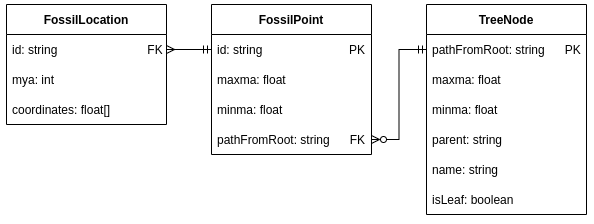
\includegraphics[width=0.4\textwidth]{figures/technical_solution/er}
	\caption{An entity relationship diagram of the database.}
	\label{fig:er}
\end{figure}

\section{Back-end query processing} \label{sec:tec_backend}
The back-end is responsible for processing the data queries requested by user actions, and sending the result to the front-end. How the queries are resolved is explained in this sub-section. There are two main queries to carry out: 1, given a time range and tree parameters, obtain a tree of life with fossil IDs attached to each node, and 2, obtain the locations of the fossil records given their IDs and a time point. \\

The first query returns a fossil-attached tree under a requested root node. The following parameters are passed to the database: 
\begin{itemize}
	\item \textit{searchTerm}: the root node's name or pathFromRoot
	\item \textit{maxma}: the start of the selected time period
	\item \textit{minma}: the end of the selected time period
	\item \textit{maxElement}: the maximum number of siblings to retrieve under each node
	\item \textit{depth}: the number of tree layers to retrieve 
\end{itemize}

The resulted tree should be rooted by the requested node, with a depth no greater than the parameter \emph{depth}. The number of children under each node is no greater than the number of \emph{maxElement}. The IDs of fossils that exist during the time period are also attached to each node. The returned tree is an array of nodes with the following fields:  

\begin{itemize}
	\item \textit{pathFromRoot}: the unique identifier of the node
	\item \textit{name}: the node's name
	\item \textit{parent}: the \textit{pathFromRoot} value of its parent
	\item \textit{isLeaf}: a boolean value indicating if the node is a leaf node with respect to the returned tree
	\item \textit{fossils}: the IDs of fossil records existing during the requested time period that either are attached to this node (if the node is not a leaf node) or belong to the node's subtree (if the node is a leaf node)
\end{itemize}

To retrieve the tree, we first find the requested root node by searching for either its \emph{name} or \emph{pathFromRoot} in \emph{TreeNode}. The \emph{name} is passed from user input in a search bar and the \emph{pathFromRoot} is passed from a clicking event on the tree graph. Since the first letter of all names in \emph{TreeNode} are capitalized, we capitalize the first letter in \emph{name} in case it is not, before performing the search. If the \emph{searchTerm} is a dash-separated name, then it is one of the unique names selected by users from the front-end's search bar. Then we only return the root node whose \emph{pathFromRoot} contains the name to the right of the dash sign. For instance, if the \emph{searchTerm} is "Corydalis-Animalia", two results can be returned when searching by the name "Corydalis". However, we only return the result whose \emph{pathFromRoot} contains "Animalia", leaving the other "Corydalis" that is in fact under "Plantae".\\

The \emph{parent} value of the root node is set to null since although it may have a parent in the complete tree of life, it acts as the root of the tree to be returned. The fossil IDs attached to the root node are also appended. We then recursively search for its children by using the \emph{parent} field and append the children nodes to the result. The recursion terminates until reaching the requested depth or encountering nodes with no children left. When processing a certain node during the recursion, we compute the \emph{isLeaf} value in the following way. If this node has no children in the complete tree of life (\emph{i.e.}, this node's \emph{isLeaf} value in database's \emph{TreeNode} is already true), then it is certainly a leaf node in the tree under construction. However, if the iteration is on the maximum depth, then the node is a leaf node with respect to the tree under construction, whether or not it has children in the complete tree of life. When it is a leaf node, we search for the IDs of all fossils belonging to its subtree. This can be easily performed with string matching the \emph{pathFromRoot} of the fossil records in database's \emph{FossilPoint} using a regular expression since all desired fossils' paths begin with the \emph{pathFromRoot} of the current node. When the node is not a leaf node, we only attach fossils that are strictly associated with this node, by exact string matching of \emph{pathFromRoot} between this node and the fossil records. To improve efficiency, the sibling nodes are filtered before continuing to the next recursion level. A count value is computed for each sibling node, which is the number of fossil records belonging to its subtree that is present during the time period. Then the siblings are ranked in descending order, and the top \emph{maxElement} number of siblings are kept. \\

The second query receives a time point of interest and an array of nodes with fossil IDs attached, which is a result of the first query. However, only the relevant fields are passed: 
\begin{itemize}
	\item \textit{name}: the node's name
	\item \textit{fossils}: the IDs of fossils attached to the node (if it is a lead node) or its subtree (if it is not a leaf node)
\end{itemize}

From \emph{FossilLocation}, we retrieve the fossils' coordinates by their IDs and time point, and organize the result in an array. Each item has the following fields:

\begin{itemize}
	\item \textit{id}: the fossil record's ID
	\item \textit{coordinate}: the fossil location at the time point, in the form of [latitude, longitude]
	\item \textit{name}: the name to which the fossil record is associated in the current tree
	\item \textit{mya}: the requested time point 
\end{itemize}

\section{Front-end development} \label{sec:tec_frontend}
This section introduces the design solution for the front-end, which includes a global states section that locally stores variables to which different components in the user interface have access, and the user interface where viewers interactively explore the visualized data. The user interface is in turn divided into a time control component, a map component, and a tree component. 
\subsection{The global states}\label{subsec:tec_frontend_global_states}
The global states serve as the intermediate agents between the user interface and the back-end, and between different components of the user interface. As shown in Figure \ref{fig:architecture}, global states include \emph{Time parameters}, \emph{Tree parameters} and \emph{Current tree and fossils}. \\

\emph{Time parameters}. Time parameters store a time period and a time point. Upon a time-related request from the user interface, certain values of time parameters are updated, and new data queries are triggered. When only the time point is changed, new fossil location data is queried using time point and the fossil IDs stored in \emph{Current tree and fossil ID}, and new map data is loaded from static files in the back-end. When the time period is changed, a time point that represents the period is also calculated. Data on a new tree and attached fossil IDs are queried in regarding the time period, before storing the new result by updating \emph{Current tree and fossil ID}. Due to the updated time point value, data on the map and fossil location is also queried. \\

\emph{Tree parameters}. Tree parameters keep the record of how the tree is customized by the users. It includes the requested depth, the maximal number of children to retrieve under a given node, and the name or the path of the node to search for. When any of the parameters are changed as a result of user actions, combining with the time period information in \emph{time parameters}, a new data query is sent to compute a customized tree of interest formed by fossils found in the time period, and the returned data containing both the tree nodes and the attached fossil IDs is stored in \emph{Current tree and fossil ID}. Lastly, in the user interface, when a user hovers on a node in the tree graph or a fossil point on the map, the identity of the node is recorded as a parameter, for both tree and map to be aware of, which is required for the communication between the two components. The tree parameters are also responsible for the communication between map and tree components. When a user hovers the mouse on either a node in the tree graph or a fossil point attached to a certain node on the map, a parameter also records the identity (\emph{pathFromRoot} value) of the tree node. As a result, the information on which node is being highlighted is shared with the other component, which also elicits a highlighting effect as a response. \\

\emph{Current tree and fossil ID}. This global state variable stores information on current tree nodes with fossil IDs attached. It mainly serves two purposes. When users are interested in viewing how the same fossil points move as a result of plate movement through time, they change the time point value in \emph{time parameters}, triggering a data query for new fossil locations with the pre-stored fossil ID values. Under this circumstance, the fossil IDs remain constant, it is thus more efficient to store them locally than re-querying upon a new time point. In addition, the colors of nodes shown in the tree component are consistent with the colors of their attached fossil points shown in the map component. As a result, upon receiving new tree and fossil ID data from the database, instead of sending directly to the tree component in the user interface for rendering, we compute the colors before storing this information in \emph{Current tree and fossil ID}. Thereby, the color values are calculated only once and are shared by both map and tree components when they render fossil points and the tree respectively. The coloring of the tree node is determined as follows. The current root node is in black. Its descendants are assigned with one of the five distinctive colors. The assignment initiates from the children of the root node, by visiting each node in a breath-first-search manner. A color is removed from the palette when it is assigned to a node. After all five colors are used, if the new node being visited is still a child of the current root, then the last of the five colors is assigned to this node; otherwise, we assign the same color as its parent, which must already have one of the five colors, as the parent has been visited and assigned with a color in the breath-first-search process. 

\subsection{The user interface: time control component}\label{subsec:tec_frontend_time}

\begin{figure}[h]
	\centering
	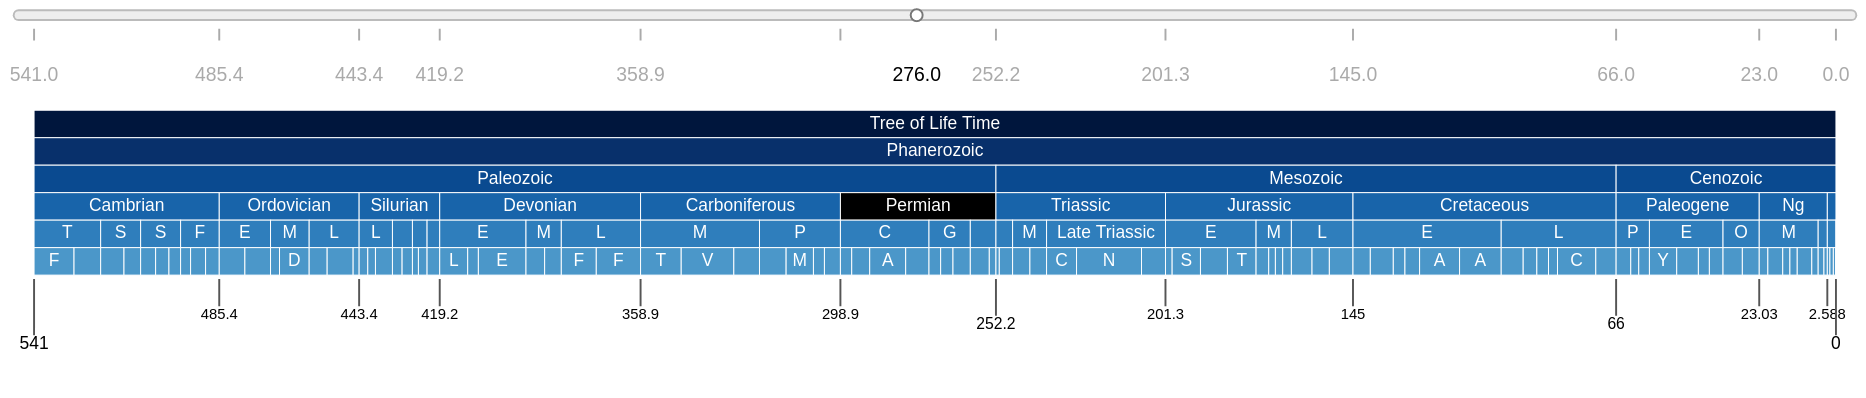
\includegraphics[width=0.9\textwidth]{figures/technical_solution/time_control/time_control_overview}
	\caption{An overview of the time control component. A timescale table displays all time periods of the Phanerozoic that are organized hierarchically in five layers. When selecting a time period, \emph{i.e.} "Permian", its cell is marked in black. Some tick values are shown below the table, marking the start and end years of all time periods on the third layer, in the unit of million years. There is a scroll bar on the top that allows users to drag, in order to view the world map and the fossil locations of a later time than the selected time period.}
	\label{fig:time_control_overview}
\end{figure}

The time control component shown in Figure \ref{fig:time_control_overview} sits at the bottom of the user interface. It allows users to control the map and tree components by either clicking in the timescale table or dragging the scroll bar. The first functionality is shown in Figure \ref{fig:time_control_period}. Users can pick a time period of interest to view the tree and fossil points during that period by clicking a cell in the timetable. Only a time period on or below the third layer (Period) can be selected, in order to avoid requesting fossil data spanning hundreds of millions of years at a time, which may exceed the size of the heap memory. When a time period is selected, a time point at which the world map and the fossil locations will be queried is also calculated. This time point is intended for representing the geology during the time period. Due to the hierarchical nature of the timescale, a certain time point must belong to a time period in the fifth layer (Age). We intend to show the name of this Age, since it is of the highest detail. When an Age is selected, the time point is simply the middle value between the start and end year, rounded up to an integer (Figure \ref{fig:time_period_fifth_layer}). Otherwise, the middle value of the time period is calculated, and we search for the Age where this calculated middle value falls into. Then, the middle integer value of that Age is used as the time point (Figure \ref{fig:time_period_third_layer}). The second functionality is shown in Figure \ref{fig:time_control_point}. Users can pick a time point that is later than the selected time period to view how fossil locations are shifted with the continents, by dragging the scroll bar on the top. Those time points are the middle values of all Ages later than the current time point, rounded up to an integer. \\

The entire Phanerozoic Eon spans over 500 million years, whereas certain time periods, especially those of lower layers, are only a hundredth of that length. Without dynamic scaling of the timetable, it is difficult to have a clear view or easy accessibility of the time periods in lower units. A solution is demonstrated in Figure \ref{fig:time_control_hover}. When hovering on a time period on the third (Period) layer or lower, a zooming effect takes place, where all time periods from the Period layer and below are elongated, such that the Period cell occupies 90\% length of its immediate ancestor (an Era cell). As a result, labels indicating the start and end year of the shortest time periods on the Age layer can also be shown. To further highlight the time period, when hovering on it, the opacity of all other time periods that are not in the path to the common ancestor "Phanerozoic" is decreased, and a small pop-up note also shows its name as a path from the common ancestor. \\


\begin{figure}[h]
	\centering
	\subfigure[The time period "Phanerozoic -> Cenozoic -> Paleogene -> Eocene -> Ypresian" is selected. Since this is a time period in the lowest layer (Age), the timelines below both map and tree show the name of this time period. The map in fact shows the continents and fossil locations at the middle point of this period.]{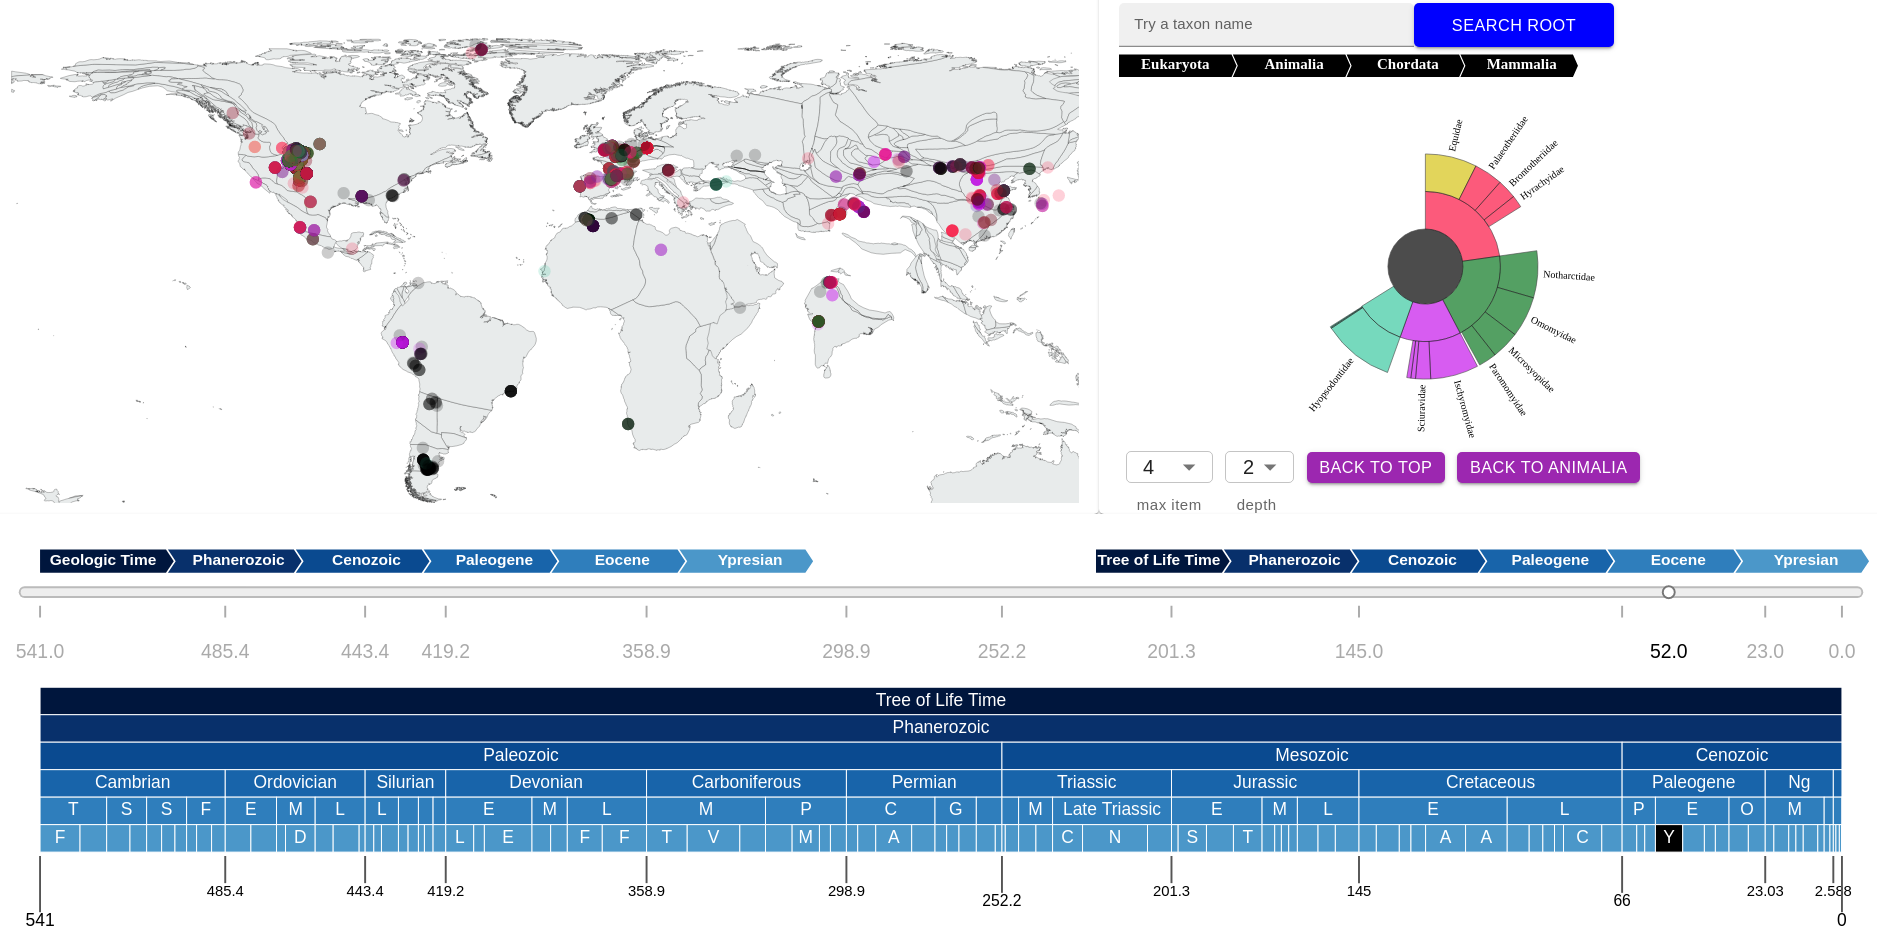
\includegraphics[width=0.48\textwidth]{figures/technical_solution/time_control/time_period_fifth_layer} \label{fig:time_period_fifth_layer}}
	\hfill
	\subfigure[The time period "Phanerozoic -> Cenozoic -> Paleogene" is selected. This time period is not in the lowest layer (it is a Period), but its middle value falls into "Phanerozoic -> Cenozoic -> Paleogene -> Eocene -> Lutetian", a time period on the lowest Age layer. Therefore, in the map component, Lutetian is the Age that represents the selected Paleogene, and its name is shown beneath the map on the left. We then take the middle value of Lutetian as the time point at which the continents were shaped and the fossils were located. ]{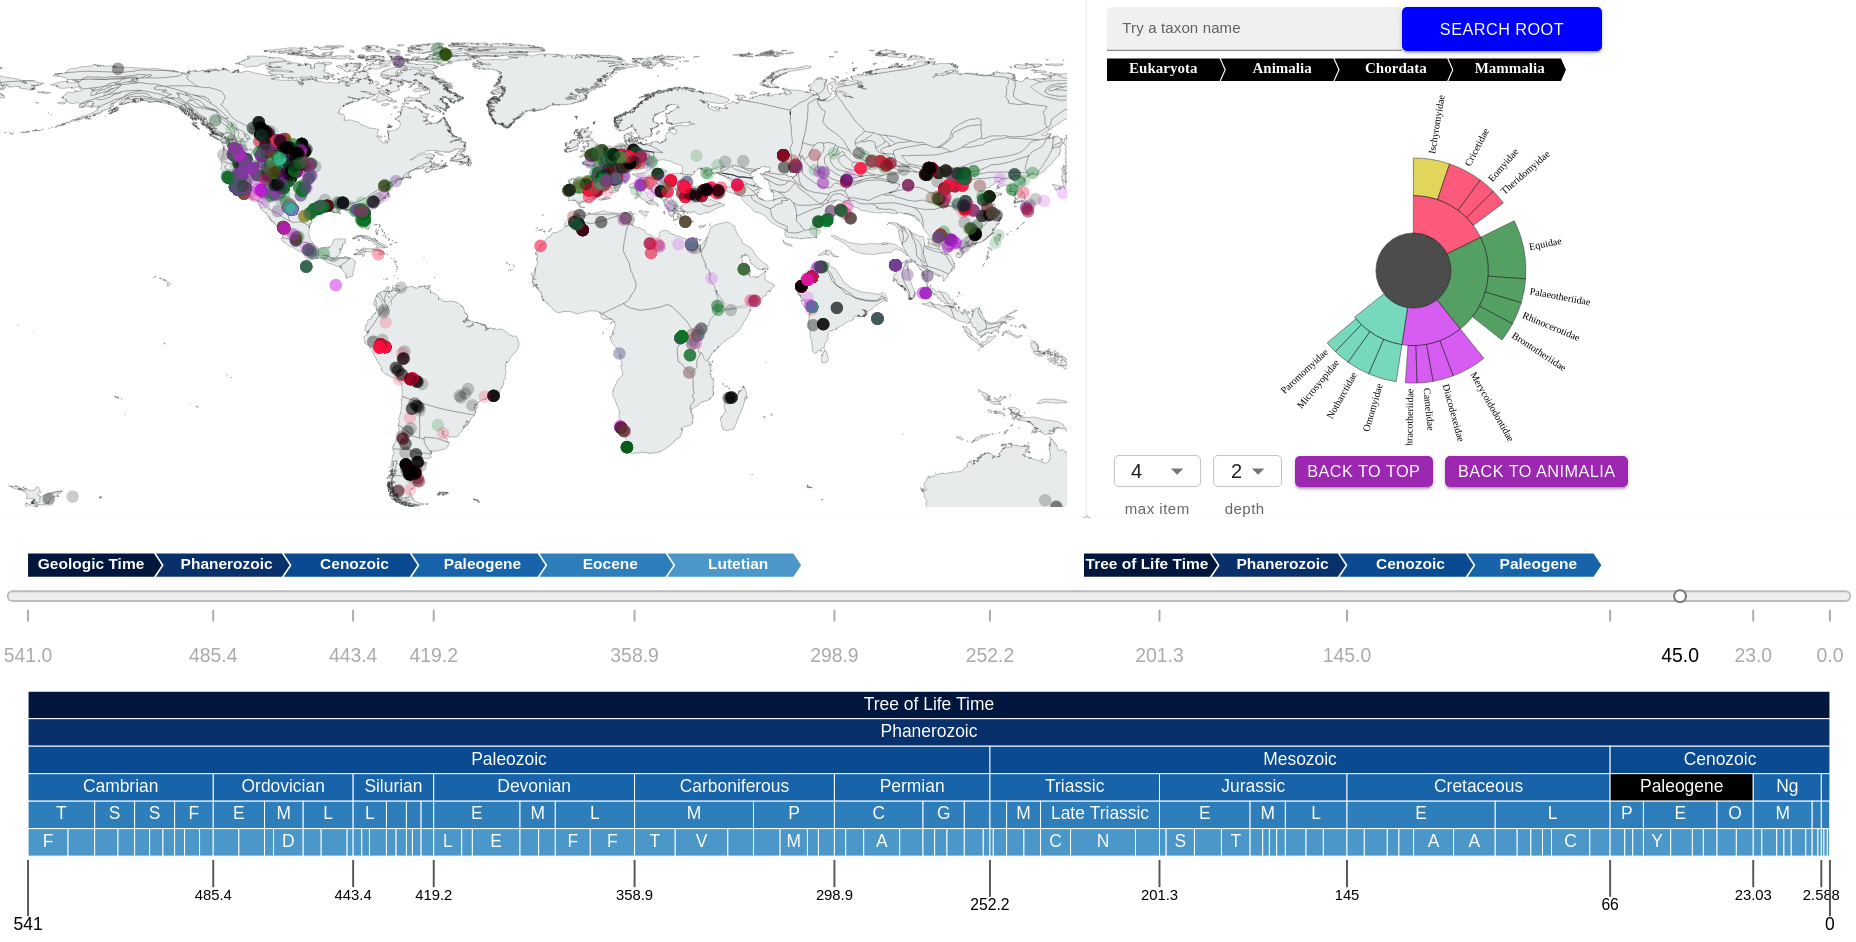
\includegraphics[width=0.48\textwidth]{figures/technical_solution/time_control/time_period_third_layer} \label{fig:time_period_third_layer}}
	\caption{The timescale functionality of the time control panel. Users can select a period in the timescale to view the map and tree during this time period. The tree of life is always in accordance with the selected time period, whereas when the time period is not on the Age layer in the timescale, the map component picks the middle value of the Age in which the middle value of the select time period falls.}
	\label{fig:time_control_period}
\end{figure}

\begin{figure}[h!]
	\centering
	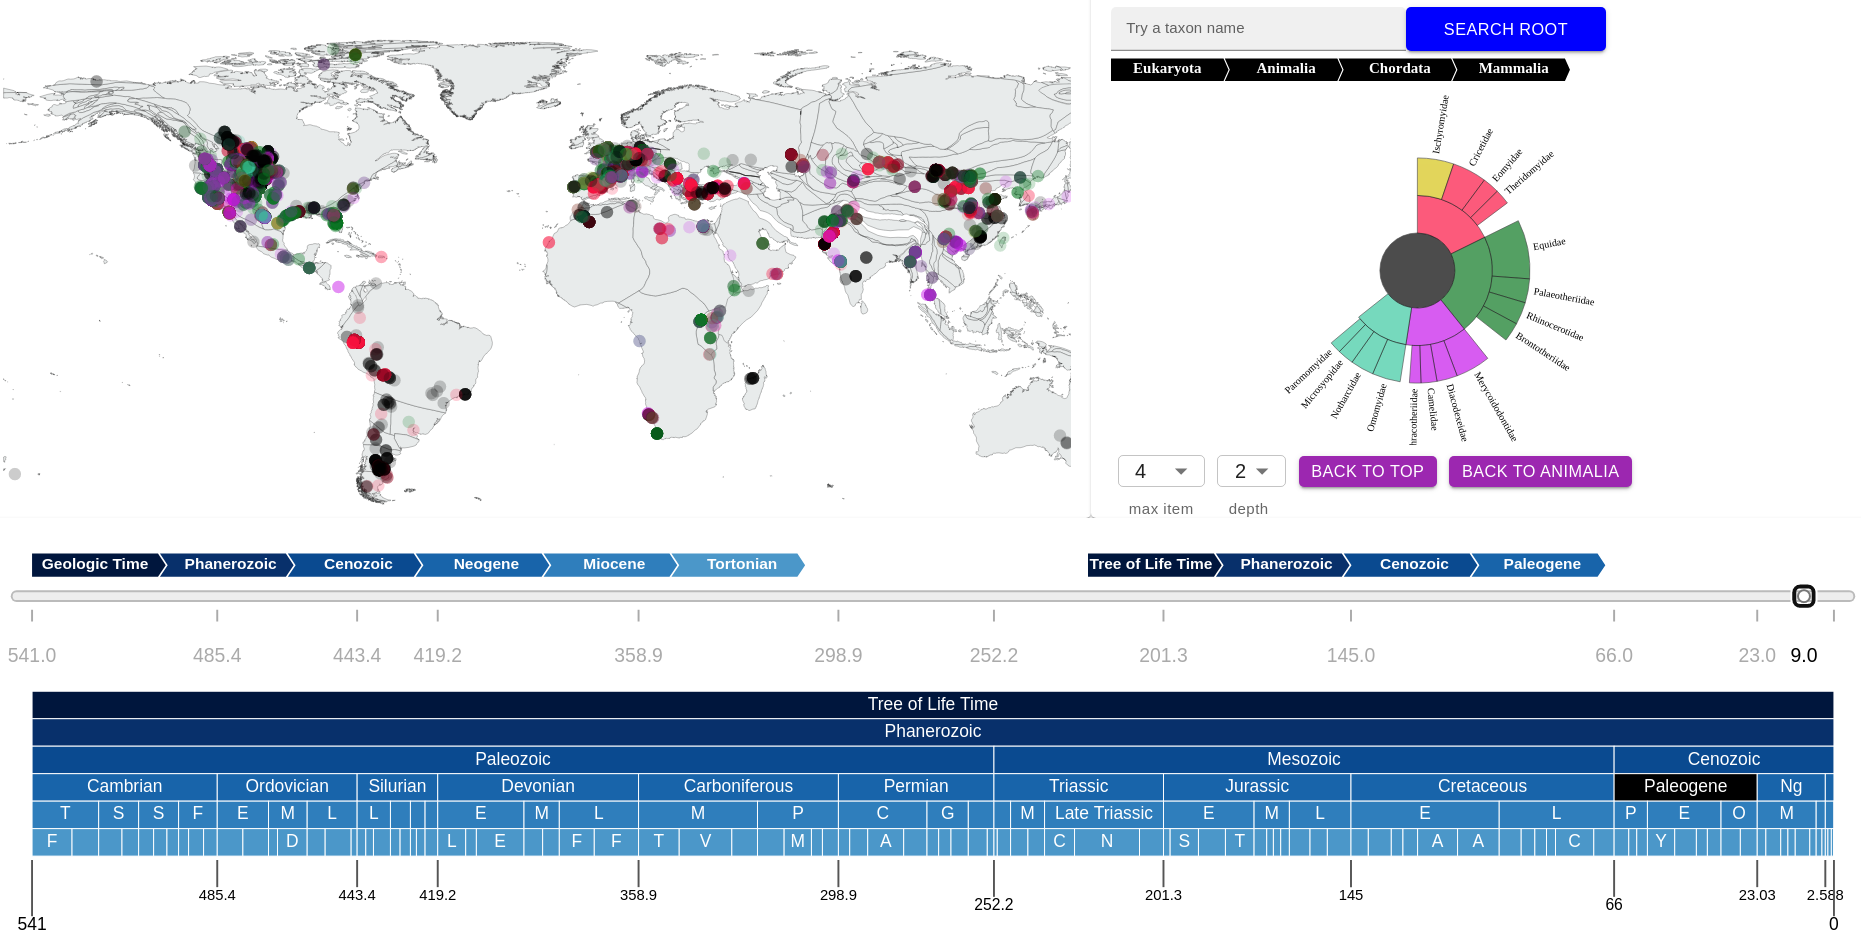
\includegraphics[width=0.7\textwidth]{figures/technical_solution/time_control/time_point}
	\caption{The scroll bar functionality of the time control panel. Users can drag the scroll bar to a later time point than the currently selected time period, in order to track how the continents and the fossil points move due to plate motion. From the time table and the breadcrumb beneath the tree, we can see that the tree of life and the attached fossils are still with respect to the selected "Phanerozoic -> Cenozoic -> Paleogene". However, the number of the scroll bar and the breadcrumb beneath the map imply that the scroll bar has brought the world map to a more recent time point at 9 million years ago, which is during "Phanerozoic -> Cenozoic -> Neogene -> Miocene -> Tortonian".}
	\label{fig:time_control_point}
\end{figure}

\begin{figure}[h]
	\centering
	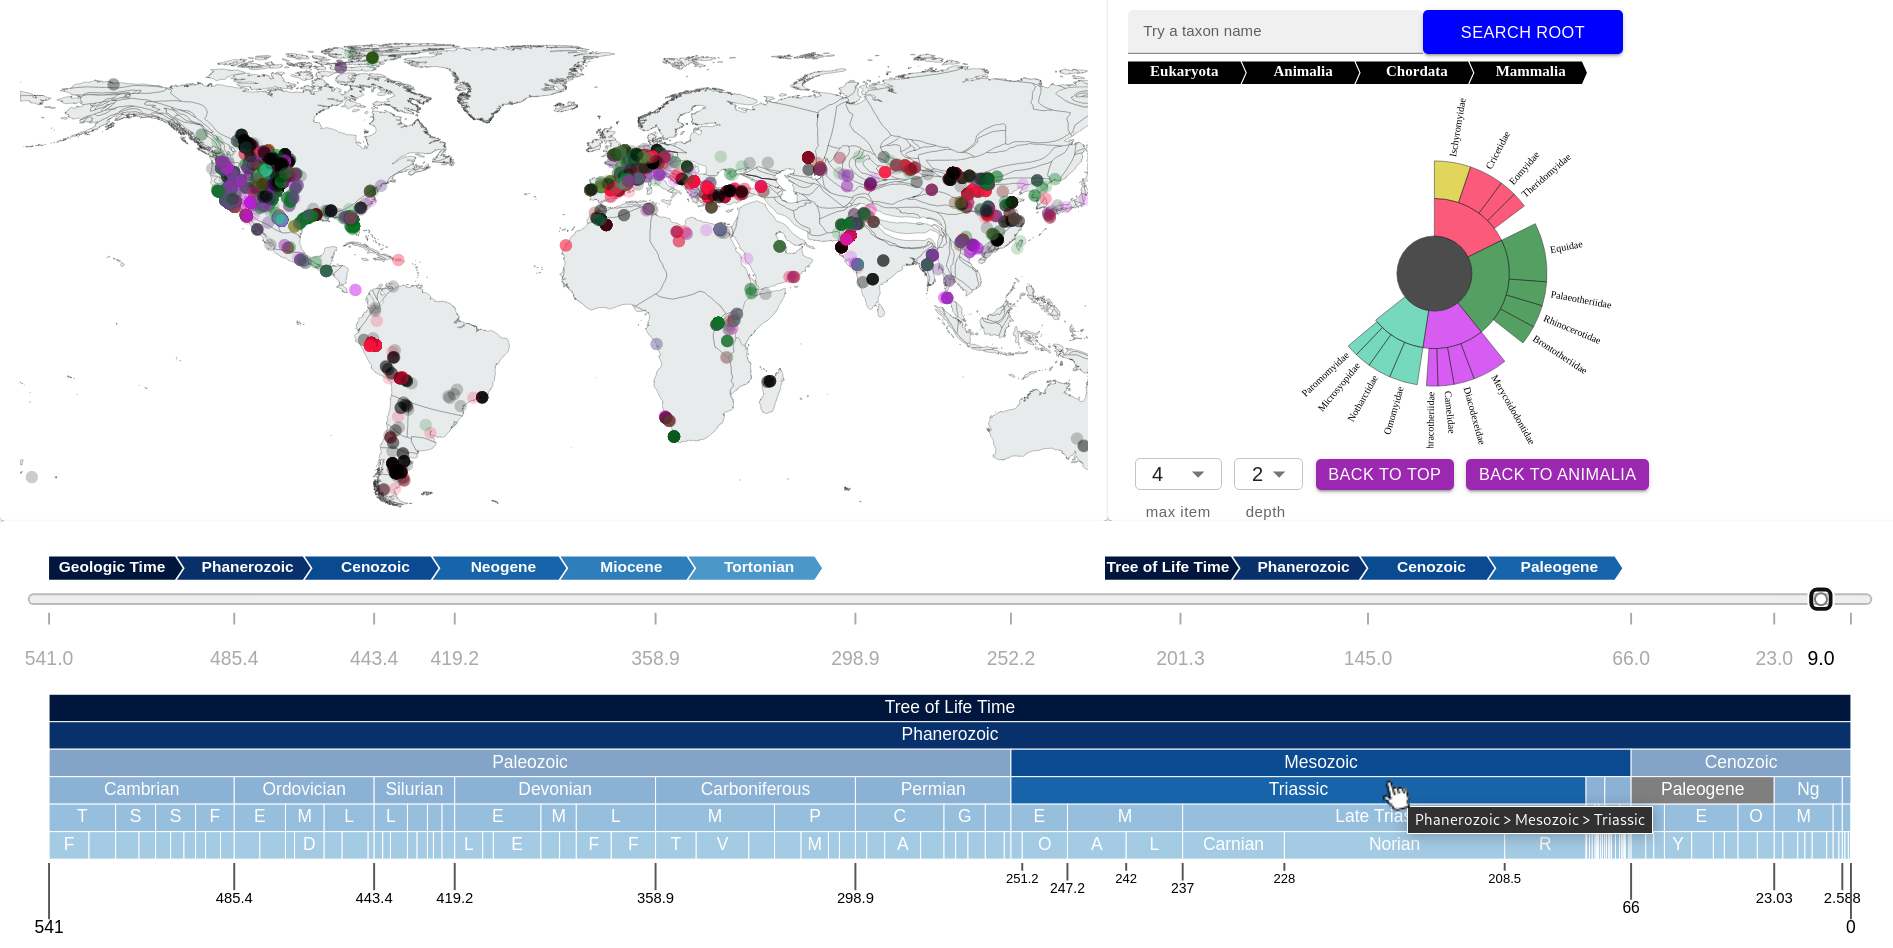
\includegraphics[width=0.7\textwidth]{figures/technical_solution/time_control/time_hover}
	\caption{The zooming and highlighting effect of the timescale upon hovering. When users hover on a particular time period, a pop-up note with its name shows next to the pointer, and all other time periods that are not in its path to Phanerozoic are decreased in opacity. The selected "Triassic" belongs to a period on the third layer or below, as a result, a zooming effect takes place. All time periods at or below "Triassic" are proportionally elongated such that "Triassic" takes up 90\% the length of its parent "Mesozoic". Due to this expansion, the tick values can now show all start and end years on the lowest layers. }
	\label{fig:time_control_hover}
\end{figure}

\clearpage
\subsection{The user interface: tree component}\label{subsec:tec_frontend_tree}
\begin{figure}[h]
	\centering
	\subfigure[A tree component showing "Plantae" and its descendants during "Quaternary" time period.  ]{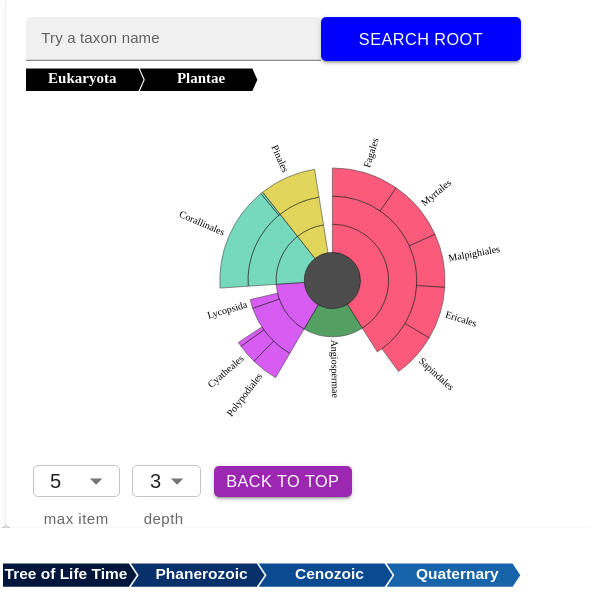
\includegraphics[width=0.35\textwidth]{figures/technical_solution/tree/tree}\label{fig:tree_a}}
	\hfill
	\subfigure[A tree component showing "Primates" during "Quaternary" time period. The pointer is hovering on ancestor "Mammalia". It is possible to navigate to any ancestor of the current node in the breadcrumb by clicking. ]{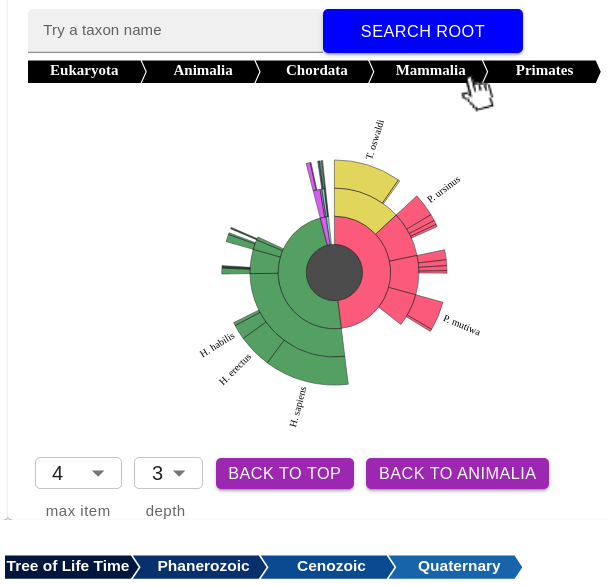
\includegraphics[width=0.35\textwidth]{figures/technical_solution/tree/tree_breadcrumb}\label{fig:tree_b}} 
	\subfigure[The tree is the same as (b). The pointer is hovering on "BACK TO TOP" button, which directs the users to the top of the tree "Eukaryota". ]{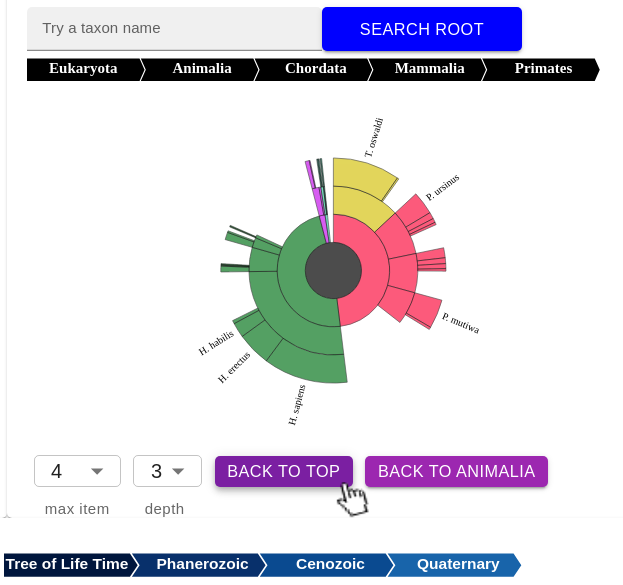
\includegraphics[width=0.35\textwidth]{figures/technical_solution/tree/tree_backtotop}\label{fig:tree_c}}
	\hfill
	\subfigure[The tree is the same as (b). The pointer is hovering on "BACK TO ANIMALIA". Animalia is the \emph{depth}'th ancestor of the current root. Note that this button is absent in (a), since the current root does not have a \emph{depth}'th ancestor. ]{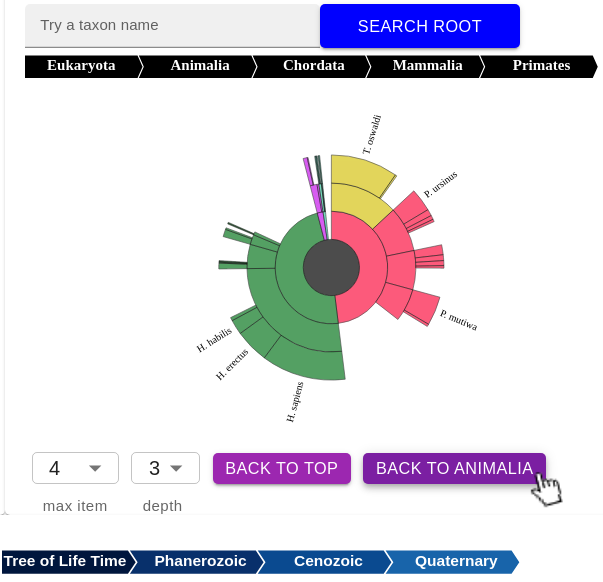
\includegraphics[width=0.35\textwidth]{figures/technical_solution/tree/tree_backup}\label{fig:tree_d}} 
	\caption{The tree component of the user interface. From top to bottom, it has a search bar for user input, a breadcrumb in black that shows the position of the current root, a sunburst graph that reflects the prevalence of each node during the time period via arc angles, a control panel for tree customization, and a breadcrumb showing the current time period.}
	\label{fig:tree}
\end{figure}
The tree component is on the right of the user interface. It shows the current tree of interest, while providing options to customize the tree. A typical tree component is seen in Figure \ref{fig:tree_a}. A search bar is located on the top, where users can search for a name. Below, a line of breadcrumb indicates the location of the current root in the complete tree of life, by showing all of its ancestors in a path from the common root. Each ancestor can be visited by clicking (Figure \ref{fig:tree_b}). Since the ancestor nodes are upstream of the current root, they are colored in black, to distinguish from the current root's descendants in other colors. The tree is rendered as a sunburst graph from the global state variable \emph{Current tree and fossils} addressed in sub-section \ref{subsec:tec_frontend_global_states}, which contains information on a node's name, color and fossils. \\

To demonstrate the prevalence of a certain taxonomy during the selected time period, the angle of each node's arc reflects the number of fossils attached to its subtree. The current node under inspection is the root of the tree being displayed, as a consequence, it is a full circle, since it includes all fossils in its subtree. The arc angles of sibling nodes are proportional to the ratio between the number of fossils in their respective subtree, and the number of fossils included in their parent's subtree. To calculate the number of fossils under a given node's subtree, we recursively sum up the fossil counts from leaf nodes to the current root node, by the number of fossils attached to each node. Note that when performing the sum up, if the node is a leaf node, we sum up by all fossils under its subtree, however, when the node is not a leaf node, we sum up by the fossils that are attached to the node. This is because if we still sum up by the fossils belonging to its subtree, we are double-counting the fossils, as each of its children is already summed up by the fossils under their respective subtree. \emph{Current tree and fossils} conveniently stores fossils attached to a node (for non-leaf nodes), or fossils associated with the node's subtree (for leaf nodes). Therefore, when performing the sum up at the front-end, no further processing is needed to distinguish if we are counting the fossils with respect to only a node, or its subtree. \\
\begin{figure}[h]
	\centering
	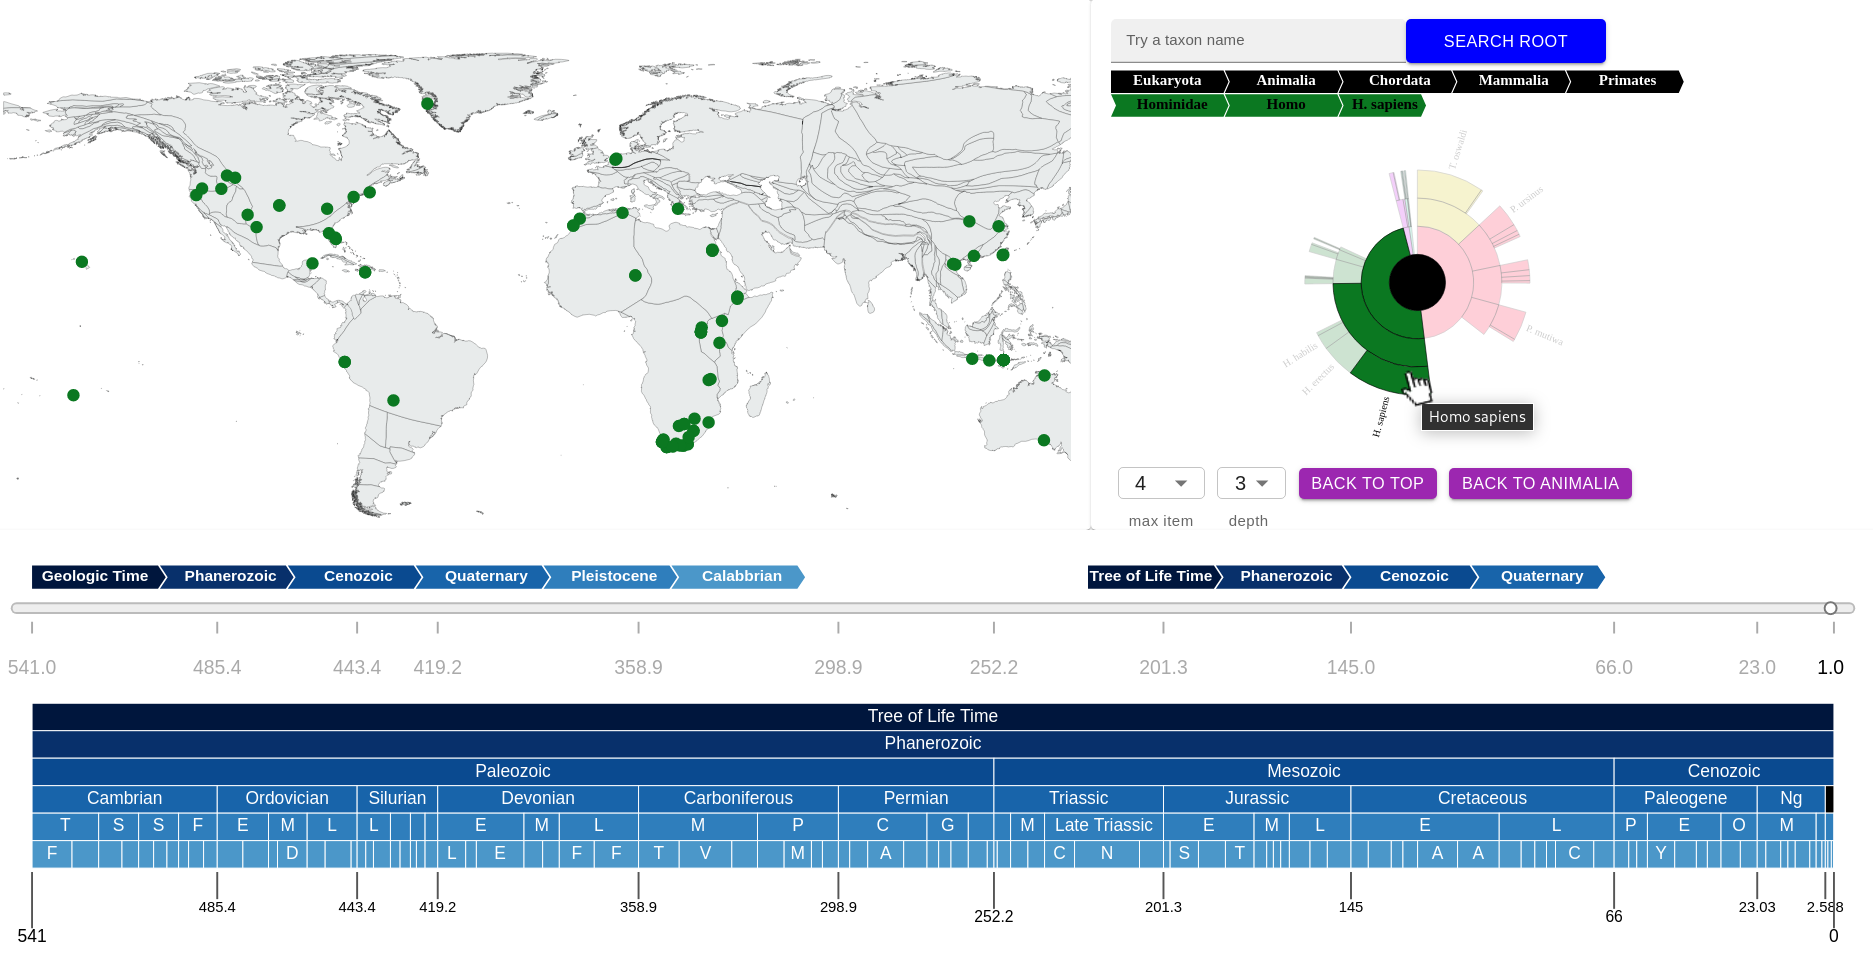
\includegraphics[width=0.6\textwidth]{figures/technical_solution/tree/tree_hover}
	\caption{The tree's visual effect upon user hovering on a node. The tree is the same as in Figure \ref{fig:tree_b}. When a user hovers on "Homo sapiens", a pop-up note shows its name, and an additional breadcrumb in the color that is consistent with that of the tree appears, indicating the position of the hovered node in the complete tree. The nodes that are in its path to the current root are in full opacity, whereas all other nodes have decreased opacity. Most importantly, the map on the left side only shows the fossils directly attached to the hovered node, during the time when the user is hovering on it. Finally, it is possible to click on the node to navigate to the tree rooted by it. }
	\label{fig:tree_hover}
\end{figure}

To highlight a certain node of interest, we provide the following visual aids (Figure \ref{fig:tree_hover}). First, a second line of breadcrumb indicates its position from the current root node. Second, similar to the time control component highlighting effect, the opacity of other nodes is decreased, and a pop-up note informs the user of the node's name. When a node's name is too long or a node's arc is too narrow to display on the tree, the pop-up note and the dynamic breadcrumb provide an opportunity to view this name upon hovering. Finally, the hovering effect is communicated to the map component, such that only the fossil points attached to the hovered node are shown and in full opacity, to inform the users where their taxonomy of interest inhabited in the world during the selected time period. \\

\begin{figure}[h]
	\centering
	\subfigure[Upon clicking on \emph{max item}, a drop down list appears, prompting the users to select a number from 1 to 10, which is the maximal number of siblings to shown under a given node.  ]{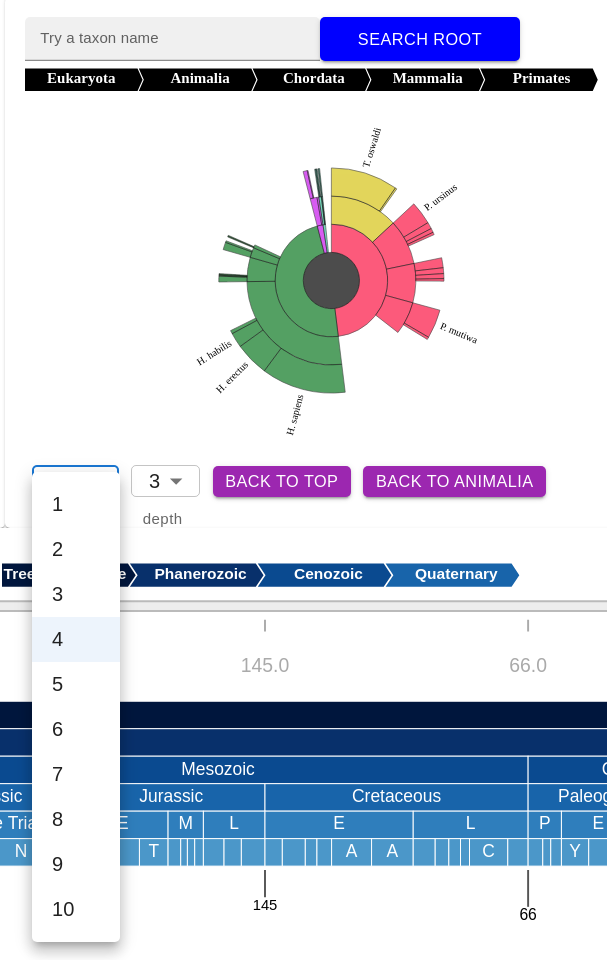
\includegraphics[width=0.35\textwidth]{figures/technical_solution/tree/tree_max_item}\label{fig:tree_dropdown_a}}
	\hfill
	\subfigure[Upon clicking on \emph{depth}, a drop down list allows users to customize the number of depth to show with respect to the current root, which is a number from 1 to 5. This number also determines which upstream ancestor to navigate to in the second "BACK TO" button. ]{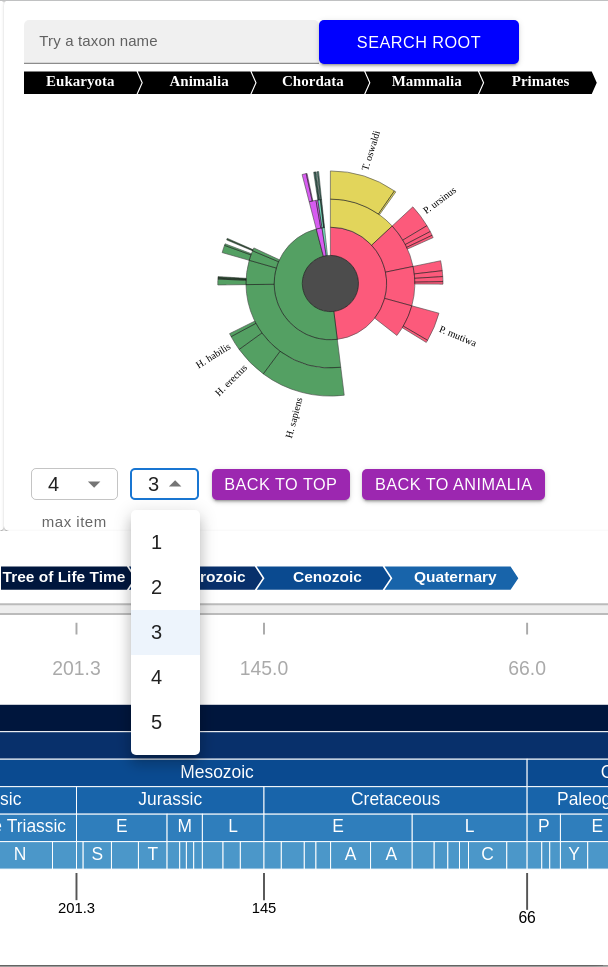
\includegraphics[width=0.35\textwidth]{figures/technical_solution/tree/tree_depth}\label{fig:tree_dropdown_b}} 
	\caption{The drop down lists in the tree's control panel.}
	\label{fig:tree_dropdown}
\end{figure}

To enable users to customize and navigate the tree, we designed a small control panel below the tree graph. If the current node is not the common root "Eukaryota", the \emph{Back to top} button directs the user to it (Figure \ref{fig:tree_c}). Clicking on the "Eukaryota" in the breadcrumb above the tree graph provides the same functionality. If the distance from the current root to "Eukaryota" is greater than the current \emph{depth}, a second button redirects the users to upstream of the current node that is its \emph{depth}'th ancestor. As an example, in Figure \ref{fig:tree_d}, the \emph{depth} value is 3, and current root is "Primates". From the breadcrumb in black, we can see that the third ancestor of "Primates" is "Animalia", hence the button in Figure \ref{fig:tree_d} that provides a quick way to navigate to it. In Figure \ref{fig:tree_a}, however, the current root is "Plantae", and it does not have a third ancestor, since its first ancestor is already the common root "Eukaryota", hence there is only a "BACK TO TOP" button. To the left of the buttons, the \emph{max item} adjusts the maximal number of elements to display under each node (Figure \ref{fig:tree_dropdown_a}), and the depth adjusts the tree's depth (Figure \ref{fig:tree_dropdown_b}). \\

Finally, when the name that the user is searching is not unique, an auto-complete function asks the user to select one of the nodes to navigate to (Figure \ref{fig:tree_autocomplete}). Note that the unique names in the drop-down list are the result from subsection \ref{subsec:tree_preparation}: the name to the right of the dashed line is the first distinctive ancestor between the two nodes.

\begin{figure}[h]
	\centering
	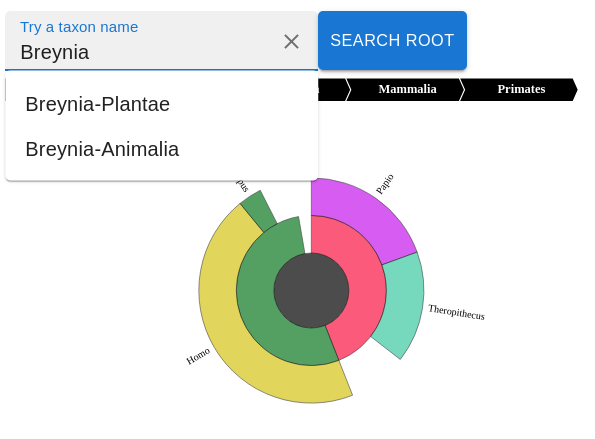
\includegraphics[width=0.6\textwidth]{figures/technical_solution/tree/autocomplete}
	\caption{The auto-complete function prompts the users to select a node to view when there are two tree nodes sharing the same search name.  }
	\label{fig:tree_autocomplete}
\end{figure}
 
\clearpage
\subsection{The user interface: map component}\label{subsec:tec_frontend_map}
\begin{figure}[h]
	\centering
	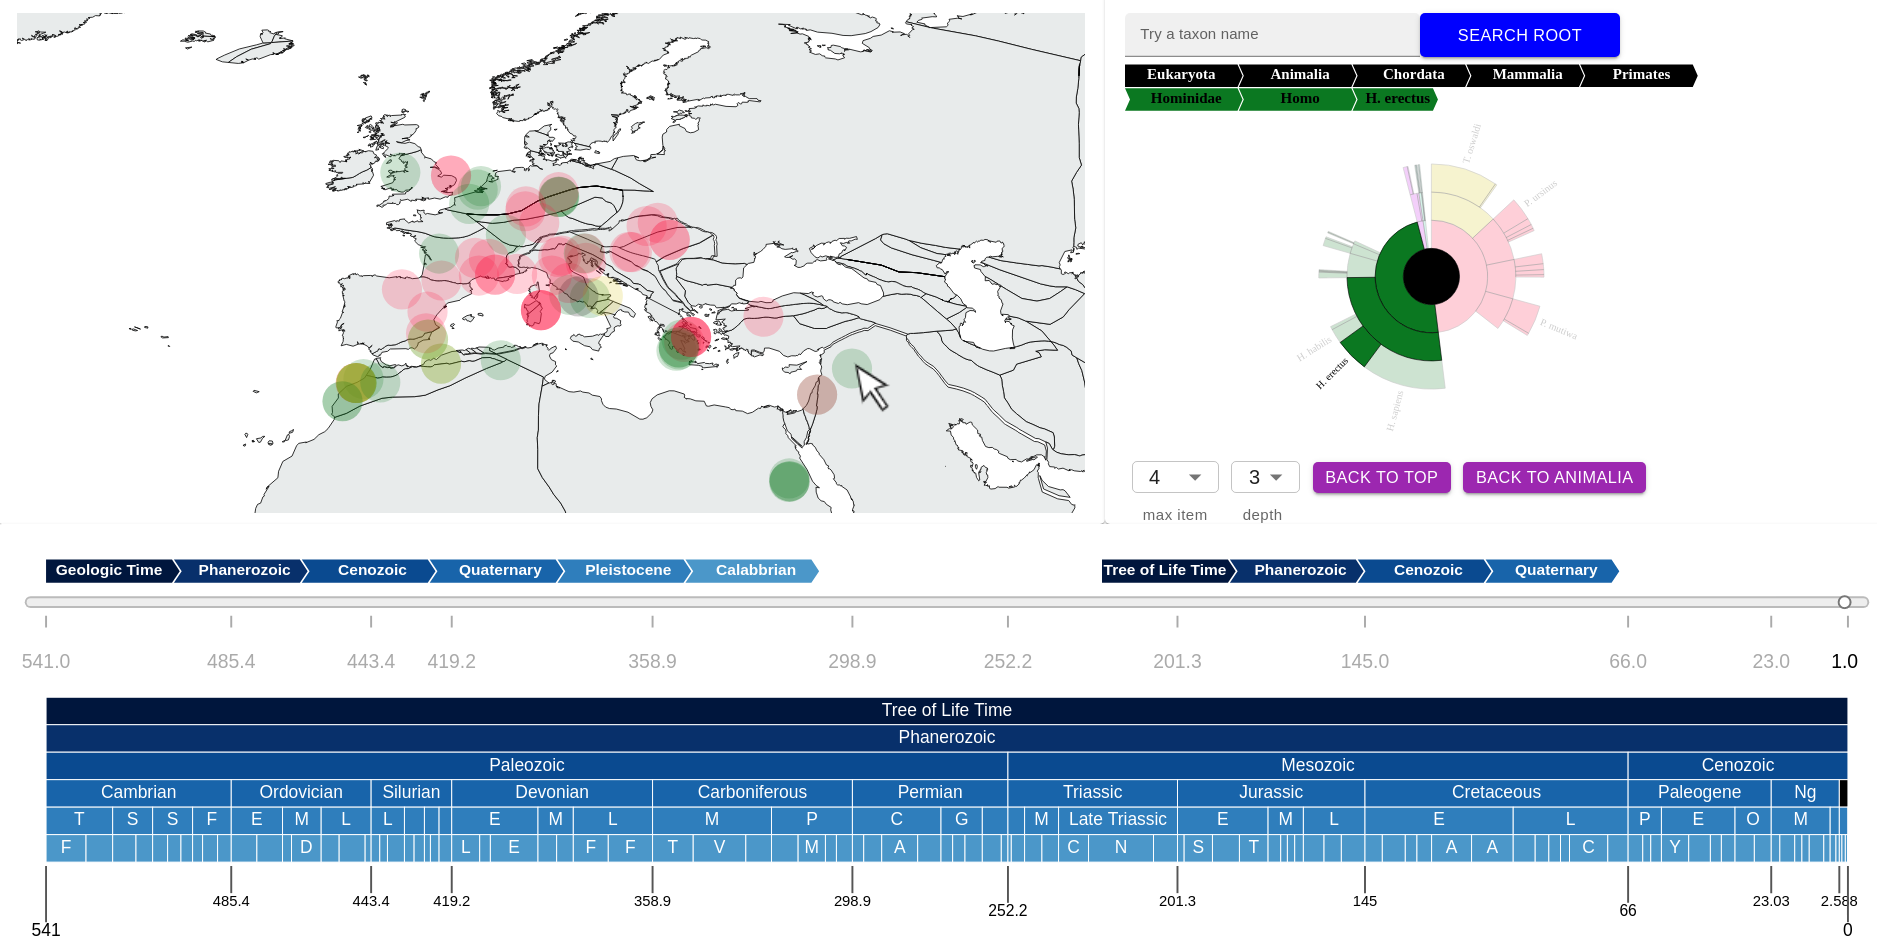
\includegraphics[width=0.7\textwidth]{figures/technical_solution/map}
	\caption{The map component of the user interface. The region around nowadays Europe is zoomed in, and the mouse is hovering on a fossil point around nowadays Middle East region. As a result, the node this fossil is attached to, which is "Homo sapien", is highlighted in the tree component, such that the node is of higher opacity, and a second breadcrumb indicates its name and path from the root. }
	\label{fig:map}
\end{figure}
The map component is on the left of the user interface. It shows the world map with fossil points at the select time point. The geological data on coastlines are provided from static files in the back-end, and the fossil coordinates are rendered directly from database's \emph{FossilLocation}, whereas their pre-computed colors are loaded from front-end in \emph{Current tree and fossils} discussed in \ref{subsec:tec_frontend_global_states}. An overview of the map component is shown in Figure \ref{fig:map}. The zooming and panning functionality enables users to view regions of interest in greater detail, and when hovering on a fossil point, the tree component shows which node it attaches to, by highlighting the node and providing a second breadcrumb that indicates its position, in a similar way as hovering on a node in the tree (Figure \ref{fig:tree_hover}). Lastly, often fossil points are of very close proximity, or even have identical locations, leading to the fact that the points can easily be on top of each other. As a solution, we decreased the opacity of the fossil points in order to reflect all fossil records' presence --- a point of higher visibility implies that there are multiple records found at or close to the location. \\



%=====================================================================
\chapter{Implementation} \label{chp:implementation}
%=====================================================================
This chapter explains how the technical solutions introduced in chapter \ref{chp:technical_solution} is implemented to produce the web application. First, the stacks used in both data processing stage and the web development stage are listed in section \ref{sec:implementation_dependencies}. Then, section \ref{sec:implementation_code_structure} describes the code structure. Next, section \ref{sec:implementation_data_processing} addresses how the data processing is implemented. Finally, section \ref{sec:implementation_web_development} explains the steps to realize the web application's structure shown in Figure \ref{fig:architecture}.
\section{Dependencies} \label{sec:implementation_dependencies}
At the data processing stage, Python3 and Pandas library are used to process the raw PBDB data to generate data on both tree and fossil information. GPlates is used to transform modern-day coordinates of both fossil records and global coastlines to ancient time points. At the web development stage, MongoDB serves as the database to store the tree and fossil data. Mongoose is used as the object document modeling (ODM) library for MongoDB and Node.js, as the back-end is written in JavaScript. GraphQL is the query language used for requesting data. The Apollo graph platform connects the front-end and the back-end, and it consists of Apollo Server, which communicates the GraphQL queries to the back-end, and Apollo Client, which manages GraghQL queries induced from actions at the front-end user interface. Axios is used to load world maps in GeoJSON by accessing a file's URL. Finally, React is the framework in which the front-end is implemented, and MaterialUI is used to style the website. d3.js is the library used for generating and manipulating the visualized data that is SVG-based. Finally, Webpack is used as the module bundler.
\section{Code structure} \label{sec:implementation_code_structure}
The code for data processing, back-end and front-end are structured as follows: 
\begin{itemize}
	\item \textbf{app/}: includes the code for building the web application.
	\begin{itemize}	
		\item \textbf{server/src/}: includes the back-end code to run the server (\emph{/index.js}), to defined the Mongoose schema (\emph{/models.js}), to define the GraphQL schema (\emph{/schema.graphql}) , and to upload the processed datasets to the database (\emph{/insertBiodiversityData.js}).
		\begin{itemize}	
			\item \textbf{resolvers/}: includes the code for resolving the queries from the front-end, \textit{i.e.}, retrieving and processed desired data from MongoDB before returning the result.
		\end{itemize}
		\item \textbf{src/}: includes the code for front-end.
		\begin{itemize}	
			\item \textbf{components/}: includes the code for different components and sub-components that the front-end framework is assembled from. The user interface consists of time control, tree and map components, and there is also a component to store global states and a component for data fetching.
		\end{itemize}
	\end{itemize}
	
	\item \textbf{data\_processing}: includes the code for processing raw data to generate the tree and fossil data, the code to further organize fossil data to prepare it for coordinate transformation through time, and the code to plot the graphs in chapter \ref{chp:results}.
\end{itemize}
\newpage
\section{Data processing}\label{sec:implementation_data_processing}
\begin{figure}[h]
	\centering
	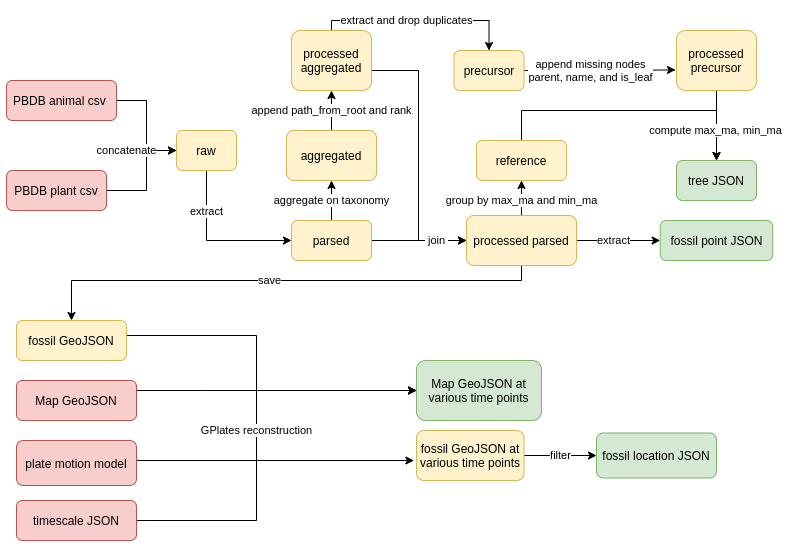
\includegraphics[width=0.7\textwidth]{figures/implementation/data_workflow}
	\caption{The data processing workflow. The unprocessed data sources are marked red; intermediate products are marked yellow; final products are marked in green. In short, The data on tree of life and fossil point is prepared from PBDB data on animal and plant fossils. The geospatial data on both map and fossil locations at different time points are prepared from GeoJSON data (unprocessed or intermediate files) and a published plate motion model using GPlates software. }
	\label{fig:data_workflow}
\end{figure}
Prior to developing the web application, we must obtain the necessary data to visualize, by implementing the strategies in section \ref{sec:tec_data_processing}. Pandas, a standard Python library specialized in data science tasks is used for this purpose. The workflow is summarized in Figure \ref{fig:data_workflow}.  First, we concatenate the PBDB \cite{peters2016paleobiology} data files for animal and plant fossil records into one file, the raw data. Then, we parsed the relevant attributes (listed in \ref{subsec:raw_data_parsing}) to form the parsed data. The rows in parsed data with identical values on all taxonomic ranks are aggregated, such each row in aggregated data has unique taxonomy information. Then, the \emph{path\_from\_root} and \emph{rank} values for each row can be calculated. This processed aggregated data with appended information now represents all tree of life nodes with at least one fossil record attached. It is further processed in the following two directions. On one hand, it is joined with the parsed data, such that every fossil record in parsed data would also have the appended information. We then extract the \emph{path\_from\_root}, \emph{occurrence\_no}, \emph{max\_ma} and \emph{min\_ma} from the parsed data to generate the \emph{fossil\_point} dataset, which is saved in a JSON file for uploading to database. On the other hand, we extract only the newly added \emph{path\_from\_root} and \emph{rank} in the processed aggregated data, before saving the unique rows in a precursor dataset in a CSV file. This precursor dataset is responsible for the preparation of the \emph{tree} dataset, as each of its rows is a node in the tree of life. Note that the precursor dataset is still missing the tree nodes that have no fossil records attached. We first iterate it to include all missing nodes in the tree of life as mentioned in sub-section \ref{subsec:tree_preparation}. Then, we compute the \emph{parent}, \emph{name} and \emph{is\_leaf} information for each row. The precursor data is now processed. Finally, we append \emph{max\_ma} and \emph{min\_ma} values for the rows. To do that, we use the processed parsed data again. As a reminder, a row in the processed parsed data represents an individual fossil record. Therefore, we group the rows with identical \emph{path\_from\_root} (\emph{i.e.}, the fossils attached to the same tree node) by 1, the maximum of all \emph{max\_ma} and 2, the minimum of all \emph{min\_ma}. We iterate through this new reference data, and for each tree node in the processed precursor data, we visit all its ancestors to update their \emph{max\_ma} and \emph{min\_ma}, as explained in \ref{subsec:tree_preparation}. The dataset on the tree is ready to be saved in JSON and uploaded to the database. \\

Concerning geospatial data processing, GPlates is used to reconstruct all modern coordinates to ancient ones. We export the processed parsed data that contains modern coordinates of each fossil record into GeoJSON format, before loading the data into the software. In addition, we also load modern plate boundaries data as GeoJSON and the simulation model that defines the kinetics of plate motion since the past 410 million years, which are both available in the work by Matthew and colleagues \cite{matthews2016global}. The timescale data is provided by PBDB \cite{peters2016paleobiology}. As a reminder, it is a hierarchical structure with five layers, and we trace all modern locations to a particular fifth layer (Age) time period. As a consequence, all ancient time points we are reconstructing are essentially the middle integer values of all Ages that are no earlier than 410 million years. GPlates assigns all fossil points to the plate that they belong to, and reconstructs those locations together with plate boundaries, using the plate motion kinetics model. All results are exported in GeoJSON. The plate boundaries files describe the world map at a particular time point. We store them as static GeoJSON files that can be directly rendered at the front-end upon requesting a certain time point. With respect to the reconstructed fossil location data, further filtering is executed. For a given fossil record, it is in fact not necessary to keep all its ancient locations. At a time period before the earliest estimated existence of a fossil, it will never appear on the map. If a time period spans longer, then it can cover more fossils. The grossest time periods that users are capable of selecting are on layer three (Period). If a time point is earlier than the start of the Period to which the fossil's \emph{max\_ma} belongs, then we can filer out its location at this time point. After filtering, we extract each fossil's ID (\emph{occurrence\_no}), coordinates, and time point in million years and store them in the \emph{fossil\_location} dataset in JSON files for uploading to the database. We use JavaScript for geospatial data processing due to its convenience when working with JSON and GeoJSON files.   

\section{Web development}\label{sec:implementation_web_development}
\subsection{Back-end} \label{subsec: implementation_backend}
The back-end provides a database to store the data prepared in section \ref{sec:implementation_data_processing}, and an API to handle the data traffic with the front-end. Although a relational database would also suffice for this project, MongoDB is used as the database of choice. It is relatively convenient to represent our prepared data in JSON with this document-oriented database system. More importantly, as a NoSQL database, the lack of data normalization enables higher horizontal scalability (\emph{i.e.}, no rigid schema). This gives a faster iteration time in the early stage of development which is highly appreciated. A lot of trials and errors are needed to decide the appropriate fields to include for both tree and fossil data. The \emph{tree}, \emph{fossil\_point} and \emph{fossil\_location} JSON files from section \ref{sec:implementation_data_processing} are uploaded to MongoDB database into collections \emph{TreeNode}, \emph{FossilPoint} and \emph{FossilLocation} respectively, as described in \ref{sec:tec_database_setup}.\\

When building the API between the data requesting front-end and the database, GraphQL is chosen as the data query language. A traditional REST API returns fixed data structures from the server, as a result, it may need to access multiple endpoints from the server, leading to over-fetching (downloading data attributes that are not actually needed) and under-fetching (accessing another endpoint since some attributes are not included in the returned result). Therefore, the APIs are designed according to the needs of the UI, such that a particular request corresponds to one endpoint from the server. However, a change of the front-end's data needs requires the corresponding back-end adjustment. GraphQL allows more rapid iterations during early development. With GraphQL, a single data query that declares all the desired fields of typed data is sent to the back-end, which returns a JSON object with only the required information. A data query is processed by a JavaScript resolver function that fetches data modeled by the ODM mongoose. The algorithms of the resolver functions are described in section \ref{sec:tec_backend}. Now, any change in the data needs would only require re-writing the relevant data queries and changing the resolver functions, which is relatively more productive. There are two possible queries, \emph{getTreeWithFossils}, which retrieves the tree with fossil IDs attached to each node, and \emph{getFossilLocations}, which retrieves the fossil coordinates data at a requested time point. The GraphQL system is implemented by the Apollo platform. It provides the Apollo server, which connects the data from MongoDB, and Apollo Client, which sends front-end data queries and returns the data to UI. An overview of the API structure is shown in Figure \ref{fig:api}. Finally, the world map at a certain time point is stored as a GeoJSON file accessed by its URL, and it can be loaded by sending an HTTP request using Axios. \\

\begin{figure}[h]
	\centering
	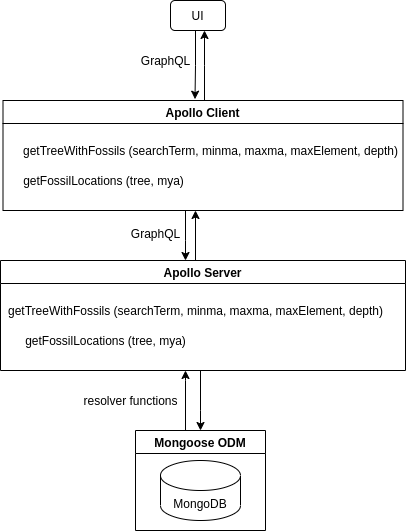
\includegraphics[width=0.5\textwidth]{figures/implementation/api}
	\caption{The API implementation. In short, Apollo Client handles GraphQL queries triggered by user action from UI. The Apollo Server then receives the GraphQL queries, which are in turn processed by resolver functions that retrieve data from Mongoose modeled data that is stored in MongoDB. The data is finally returned from the database all the way to the UI. }
	\label{fig:api}
\end{figure}

\subsection{Front-end} \label{subsec: implementation_frontend}
The front-end design from section \ref{sec:tec_frontend} is realized in a React framework. Conceptually, the front-end consists of the global states and the user interface, as seen in Figure \ref{fig:architecture} in chapter \ref{chp:technical_solution}. The implementation of global states are listed in Figure \ref{fig:global_state}. All global states can be classified into three categories. For time parameters, \emph{mya} records the time point at which to show the world map and fossil locations, while \emph{maxma} and \emph{minma} together define the time period to retrieve the fossils and to form the tree of life. For tree parameters, \emph{searchTerm} is the \emph{name} (when users request a node by typing in search bar) or \emph{pathFromRoot} (when users request a node by clicking) of the root node of the tree of interest; \emph{depth} and \emph{maxElement} are the number of layers and the max number of siblings under each node when retrieving the tree of life. Finally, \emph{mapFocusNode} and \emph{treeFocusNode} are the tree node identified by \emph{pathFromRoot} on which a user is hovering in the map (users can highlight a tree node by hovering on a fossil point that is attached to it) and tree component, respectively. They are implemented to communicate the highlighting effect in between map and tree components (Figure \ref{fig:tree_hover} and Figure \ref{fig:map}). The variable \emph{currentTree} stores all nodes of the current tree of life in an array of objects. Each object contains the information on a node's name, path, parent, color, and whether or not the node is a leaf node. The IDs of the fossils that are attached to the node (for a non-leaf node) or associated with its subtree (for a leaf node) are also stored in an array in the object. In React, variables can only be passed down from parents to children via props. Since our components are eventually assembled in a tree-like structure (Figure \ref{fig:components}), global states need to be passed down each layer to reach the component that actually needs them, leading to cumbersome code. Therefore, all global states are implemented as state variables in a React component \emph{GlobalStateContext}. A certain component gains access to the desired global states by directly importing them from \emph{GlobalStateContext} using the React hook \emph{useContext()}. \\

\begin{figure}[h]
	\centering
	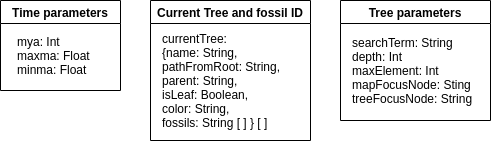
\includegraphics[width=0.7\textwidth]{figures/implementation/global_state}
	\caption{A list of all global states. The front-end's global states falls into three categories: time parameters, tree parameters and current tree and fossil ID. While time parameters and tree parameters include several variables of primitive types, current tree and fossil ID only has one variable, \emph{currentTree}, that is an array of complex objects.}
	\label{fig:global_state}
\end{figure}


Next, we introduce how the components of the user interface are assembled and how they could interact. An overview of the user interface is shown in Figure \ref{fig:components}. The user interface is presented by \emph{App}, which has one \emph{Header}, one \emph{Footer} and one \emph{TimeControl}. The \emph{TimeControl} has \emph{mya}, which is needed to show the position of the current time point in the scroll bar (Figure \ref{fig:time_control_overview}). By clicking on a selectable time period, both time point and the \emph{maxma} (the start of the time period) and \emph{minma} (the end of the time period) will be updated, triggering both a \emph{getTreeWithFossils} query for the tree, and a \emph{getFossilLocations} query for the map. Since both map and tree requires data traffic from the back-end, they both inherit from a more general \emph{DatFetcher} component for higher code re-usability. \emph{DataFetcher} is responsible for sending queries via \emph{useQuery()} that passes the appropriate \emph{queryVariables} depending on its \emph{queryName} (\emph{i.e.}, whether it is \emph{getTreeWithFossils} or \emph{getFossilLocations}). The exact \emph{queryVariables} for each query is addressed in Figure \ref{fig:api}. The \emph{data} in \emph{DataFetcher} hosts the returned data from the database, and is passed down to its children for further processing and rendering. \\

\emph{Tree} receives the tree node data, and calculates the colors for each node, before updating the result in \emph{CurrentTree}. \emph{TreeGraph} renders the tree stored in \emph{CurrentTree} in a sunburst graph. The \emph{mapFocusNode} alerts the tree graph to provide a highlight effect for the node whose fossil a user is hovering on in the map. In the meantime, when a user hovers on a node in the tree graph, it can alert the map component to highlight its fossil point by \emph{setTreeFocusNode()}. When users are intended to navigate into a node, by clicking on it from the graph or the breadcrumb above it (Figure \ref{fig:tree}), \emph{setSearchTerm()} is called, which in turn triggers new queries from the database. \\

\emph{TreeSearchName} renders the search bar above the tree graph (Figure \ref{fig:tree}). It keeps notes of what a user is typing in \emph{searchNameBuffer}, and upon clicking on the search button, \emph{setSearchTerm()} updates the name of the node of interest, which also triggers new queries. \emph{TreeGraphCustumize} renders the small control panel below the tree graph (Figure \ref{fig:tree}). It shows the current \emph{maxElement} and \emph{depth}, while updating these values when users change them in the drop down lists (Figure \ref{fig:tree_dropdown}). When users are clicking either of the "Back to" buttons, \emph{setSearchTerm()} is responsible for updating the global state variable \emph{searchTerm} with the \emph{pathFromRoot} value of the clicked node and re-directing the users to a different tree. \\

Lastly, \emph{map} renders the world map in GeoJSON, and the fossil locations returned to the \emph{data} inherited from its parent \emph{DataFetcher}. It acknowledges the colors of the fossil points from \emph{CurrentTree}, and the fossil points to highlight (as a response to user hovering in the tree component) from \emph{treeFocusNode}. \emph{setMapData()} uses Axios to load the correct GeoJSON map data according to the current \emph{mya}, before storing it in \emph{mapData} for rendering. When a user hovers on a fossil point, its attached node is updated by \emph{setMapFocusNode()} to communicate this information to \emph{TreeGraph}.

\begin{figure}[h]
	\centering
	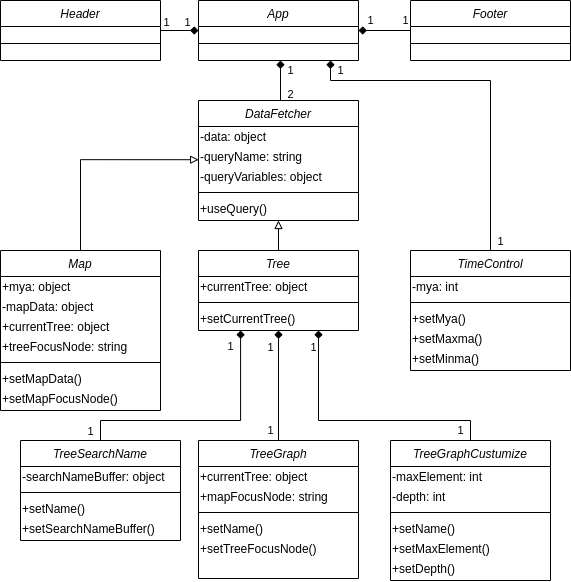
\includegraphics[width=0.7\textwidth]{figures/implementation/components}
	\caption{The implementation of the user interface by assembling different components. The user interface is the \emph{App} components, which is assembled by a \emph{Header}, a \emph{Footer}, a \emph{TimeControl} as well as \emph{Map} and \emph{tree}, which are both children of a more general \emph{DataFetcher} component. The \emph{Tree} is further broken down into three sub-components. For each component, the properties that belong to global states are marked with a "+", since they are accessible by all components.}
	\label{fig:components}
\end{figure}
%=====================================================================
\chapter{Results} \label{chp:results}
%=====================================================================
In this chapter, the results are organized into two sections. Section \ref{sec:result_data_processing} shows some characteristics of the tree and fossil data revealed after data processing. Section \ref{sec:result_data_visualization} uses some case studies to show how the web application may serve as a useful tool to explore biodiversity through time. Due to the visualization nature of the product, the results in the second section are demonstrated as screenshots.

\section{Data processing} \label{sec:result_data_processing}
There are in total 1346120 fossil records, of which 1240202 (92.13\%) are animals and merely 105918 (7.87\%) plants. Figure \ref{fig:phylum} shows a breakdown of the top five animal and plant phyla with the most number of fossils identified under them. Over the entire evolutionary history, in regard to animals (Figure \ref{fig:animal_phylum}), Mollusca (soft-bodied shell-covered invertebrates) has the highest number of fossils found, followed by Chordata (the phylum that mammals belong to), Brachiopoda (marine invertebrates with bivalve shells), Arthropoda (invertebrates with an exoskeleton and segmented body, such as scorpions) and Cnidaria (animals possessing cnidocytes, such as jellyfish and corals). In plants (Figure \ref{fig:plant_phylum}), Spermatophyta (seed plants) has the most fossils under it, followed by Pteridophyta (spore dispersing vascular plants), Coniferophyta (cone-bearing plants such as pine trees), Rhodophyta (red algae) and Angiospermae (flowering plants).

\begin{figure}[h]
	\centering
	\subfigure[The animal fossils identified under each phylum is ranked by amount in descending order and the top 5 phylums are displayed. ]{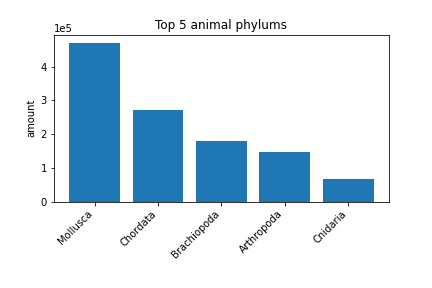
\includegraphics[width=0.45\textwidth]{figures/result/animal_phylums}\label{fig:animal_phylum}} 
	\hfill
	\subfigure[Similar to animal fossils, the top 5 plant phylums with the most amount of fossils identified under. ]{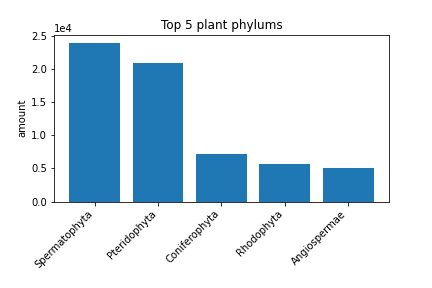
\includegraphics[width=0.45\textwidth]{figures/result/plant_phylums}\label{fig:plant_phylum}} 
	\caption{The top 5 animal and plant phylum with most fossils.}
	\label{fig:phylum}
\end{figure}

The fossil distribution in time and space is shown in Figure \ref{fig:distribution}. Fossil records are not equally distributed over the planet (Figure \ref{fig:space_distribution}). All fossils form a clear shape of the continents, indicating that proportion-wise, very few fossils are found in oceans. Furthermore, several fossil-rich areas exist, including the vast majority of North America, entire Western Europe, and most of East Asia, as well as the coastline regions of South America, Africa, and Australia. This may be due to easier fossil accessibility in those regions. The result implies a strong bias of biodiversity information favoring such regions. \\

\begin{figure}[h]
	\centering
	\subfigure[Space distribution of fossils. The longitude and latitude values of every fossil is shown on the x-axis and y-axies, forming shapes of the continents. ]{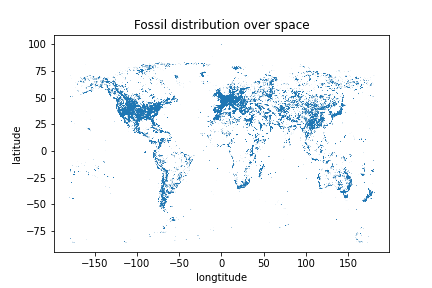
\includegraphics[width=0.45\textwidth]{figures/result/space_distribution}\label{fig:space_distribution}} 
	\hfill
	\subfigure[Time distribution of fossils during the past 600 million years. The middle value between \emph{max\_ma} and \emph{min\_ma} is comupted to represent a fossil's age, and only data in the past 600 million years is shown.  ]{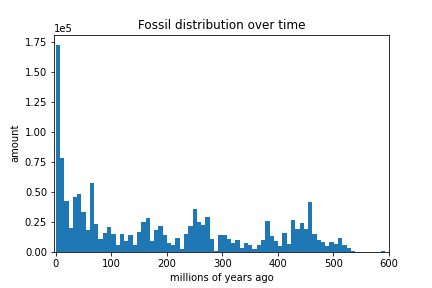
\includegraphics[width=0.45\textwidth]{figures/result/time_distribution}\label{fig:time_distribution}} 
	\caption{Fossil distribution in time and space.}
	\label{fig:distribution}
\end{figure}

\newpage
The oldest fossils in the dataset date back to 1000 million years ago. However, half of the fossils discovered are estimated to be at most 160 million years old. Each fossil is dated to an age range, with \emph{max\_ma} value indicating the maximal possible age and \emph{min\_ma} indicating the minimal. Their middle values are calculated and plotted in Figure \ref{fig:time_distribution}. An obvious bias favoring very recent (less than 10 million years ago) can be seen. In more ancient times, the fossil amount distribution tends to fluctuate. Although fossil amount is more of a measure in biomass rather than biodiversity, this fluctuation is also expected, due to the numerous mass extinction and explosion events throughout evolutionary history. The age range distribution is demonstrated in Figure \ref{fig:age_range}. There are only 444 fossil records with identical \emph{max\_ma} and \emph{min\_ma} (\emph{i.e.}, dated to a precise time point). The average age range of a fossil record is 6.80 $\pm$ 7.59 (mean $\pm$  sd) million years.

\begin{figure}[h]
	\centering
	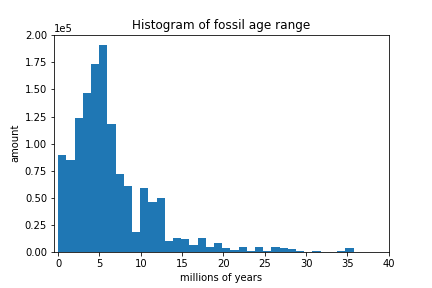
\includegraphics[width=0.45\textwidth]{figures/result/age_range}
	\caption{The fossil amount distribution over different ranges of age. The range of age is the difference between a fossil record's \emph{max\_ma} and \emph{min\_ma} values. }
	\label{fig:age_range}
\end{figure}

All fossils are organized into a tree of life with 176369 nodes, of which 147315 have at least one fossil attached. The fossil-free nodes are branch nodes that serve as the ancestors of lower-ranking nodes with attached fossils. The tree has one domain (the root "Eukaryota"), two kingdoms ("Animalia" and "Plantae"), 60 phyla, 159 classes, 1061 orders, 7305 families, 47828 genera, and 119701 species. The top five nodes with most fossils directly attached are shown in Figure \ref{fig:top_nodes}. The class "Gastropoda" is commonly known as snails and slugs, and the class "Saurischia" is a major category of dinosaurs. It can be seen that none of the nodes are on the species level, and most of the nodes are animals, as animal fossils, in general, outnumber plant fossils. \\

\begin{figure}[h]
	\centering
	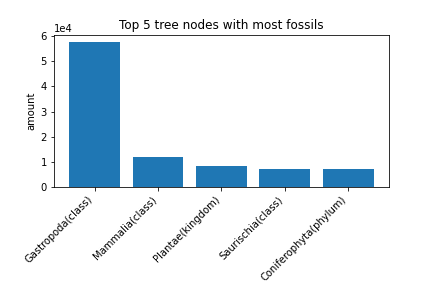
\includegraphics[width=0.45\textwidth]{figures/result/top_nodes}
	\caption{The top five tree nodes with most amount of fossils attached to. Note that this is different than in Figure \ref{fig:phylum}, which includes the fossils that are under the subtree of a certain phylum node.}
	\label{fig:top_nodes}
\end{figure}

As a reminder, when producing the tree of life using the method discussed in section \ref{subsec:fossil_preparation}, each node is uniquely identified by a \emph{path\_from\_root} string with no missing names in between. However, missing names in taxonomic ranks are very common in the raw data. As a consequence, the identified ranks of many fossils are "relocated" to a higher one, namely, the one before the first missing name. For instance, if a plant fossil is missing its phylum name but does have names on lower ranks, then it is still relocated to the kingdom node of "Plantae". Therefore, this fossil record loses some detailed taxonomic information. There are a total of 209257 (16.87\%) animals and 58874 (55.58\%) plants that suffer from this circumstance. Therefore, missing taxonomic information is a severe issue in plant records. Figure \ref{fig:relocation} shows that among all relocated animal fossils, most of them are settled on the class (54.39\%) and order (27.89\%) level, whereas most of the plant relocated fossils settle on the phylum (41.77\%), class (22.61\%), and order (22.23\%) level. 
\begin{figure}[h]
	\centering
	\subfigure[The distribution of taxonomic ranks on which relocated animal fossils are finally identified. When a fossil has taxonomic information on lower ranks but lacking names on at least one of the higher ranks, it is relocated to the rank before the first missing name. ]{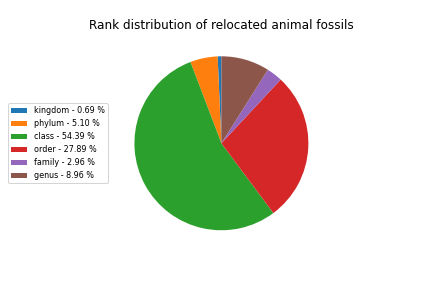
\includegraphics[width=0.45\textwidth]{figures/result/animal_relocate}\label{fig:animal_relocate}} 
	\hfill
	\subfigure[Similar to animal fossil, the distribution of ranks on relocated plant fossils. ]{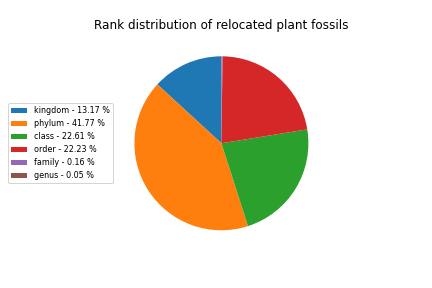
\includegraphics[width=0.45\textwidth]{figures/result/plant_relocate}\label{fig:plant_relocate}} 
	\caption{The rank distribution in fossil relocation.}
	\label{fig:relocation}
\end{figure}

\newpage
\section{Data visualization} \label{sec:result_data_visualization}
The use scenarios of the web application can be determined by a user's own need and curiosity. However, the combination of map and tree mainly enables users to observe the wax and wane of a selected taxonomy across time, as well as the change in dominance and spatial distribution of the organisms under this taxonomy. An example is seen in the development and sudden disappearance of Avetheropoda over a span of 150 million years. Avetheropoda ("bird theropods") is an order that covers dinosaurs that are relatively closely related to modern birds, as well as predatory dinosaurs, including the famous \emph{T.rex}. To begin with, we can type "Avetheropoda" in the search bar, and collect all fossils during the Early Jurassic, as seen in the breadcrumb time indicator below the tree graph in Figure \ref{fig:EJu}. During this time period, there are only a few fossils covering two families. Forwarding to Middle Jurassic, Avetheropoda has diversified greatly, as seen in the tree graph of Figure \ref{fig:MJu}. Their fossils also tend to be more well spread around the world. Late Jurassic sees an even greater amount of Avetheropoda fossils (Figure \ref{fig:LJu}). Its biodiversity in the Late Jurassic is characterized by a dominant genus (Figure \ref{fig:LJu}). This is distinctive from Middle Jurassic, during which no particular families or genera greatly outnumber others. A visual inspection of the arc angles of the tree reveals that this dominant family alone accounts for around one-third of all Avetheropoda fossils, and most of the fossils in this family belong to only one genus. When hovering on the node, we can see from the dynamic breadcrumb above the tree graph and the pop-up note that this is the genus Allosaurus from the family Allosauridae, whose fossils are found mostly in the Western United States (Figure \ref{fig:LJu_dominant}). \\

Moving on to the Cretaceous, Avetheropoda is experiencing a prosperous period. In both Early (Figure \ref{fig:ECre}) and Late Cretaceous (Figure \ref{fig:LCre}), Avetheropoda is widely spread all over the world, with even more fossils found compared to the epochs of Jurassic. This continues to Danian, the first Age (a layer-five time period) after Cretaceous (Figure \ref{fig:before_disappear}). Tyrannosaurus, the genus of the iconic dinosaur \emph{T. rex}, is highlighted by the red arrows in Figure \ref{fig:LCre} and Figure \ref{fig:before_disappear}. The relatively wide arc angle implies the prevalence of Tyrannosaurus during these times. The scroll bar at the bottom of Figure \ref{fig:before_disappear} shows that the middle value of Danian is 64 million years ago. However, when entering the next Age, Selandian, whose middle value is 60 million years ago, all Avetheropoda suddenly disappeared, except for one single fossil found on an island in the nowadays south Pacific ocean (Figure \ref{fig:disappear}). This abrupt change brought an end to Avetheropoda and also other dinosaurs, and it reflects the well-known event of a mountain-sized asteroid with a diameter of 12-kilometer hitting Earth 66 million years ago. As a result, the Age Selandian that is immediately after this incident sees few dinosaur fossils. \\

A second case study inspects Dictoyopteridiales, an order of plant present in the Permian and Triassic, that is characterized by its tongue-shaped leaves. In Figure \ref{fig:permian}, we access Dictoyopteridiales fossils during the entire Permian period. A genus Glossopteris that is marked by green points on the map can be seen dominating the southern hemisphere, while other genera are far separated from it and are inhabiting in the northern hemisphere (Figure \ref{fig:permian}). We then keep the tree of life's time in Permian (as seen in the time tables in figures of \ref{fig:plant}). Meanwhile, we use the scroll bar above the timetable to view how the same Permian fossils shift their positions through time, at an interval of around 100 million years(Figure \ref{fig:jurassic}, Figure \ref{fig:cretaceous} and Figure \ref{fig:modern}). It can be easily seen that as the supercontinent (termed "Gondwana") drifts apart since Permian, the Glossopteris fossils marked in green are gradually separated into different continents of the modern world. Although they are found in South America, the southern part of Africa, Australia, and India in the modern world (Figure \ref{fig:modern}), they were in fact joined together during the time they were alive (Figure \ref{fig:permian}). Indeed, the fossil distribution of Glossopteris is an example of how fossils could provide evidence supporting the continental drift theory \cite{schopf1970relation}. 
\begin{figure}[h]
	\centering
	\subfigure[Avetheropoda during Early Jurassic. ]{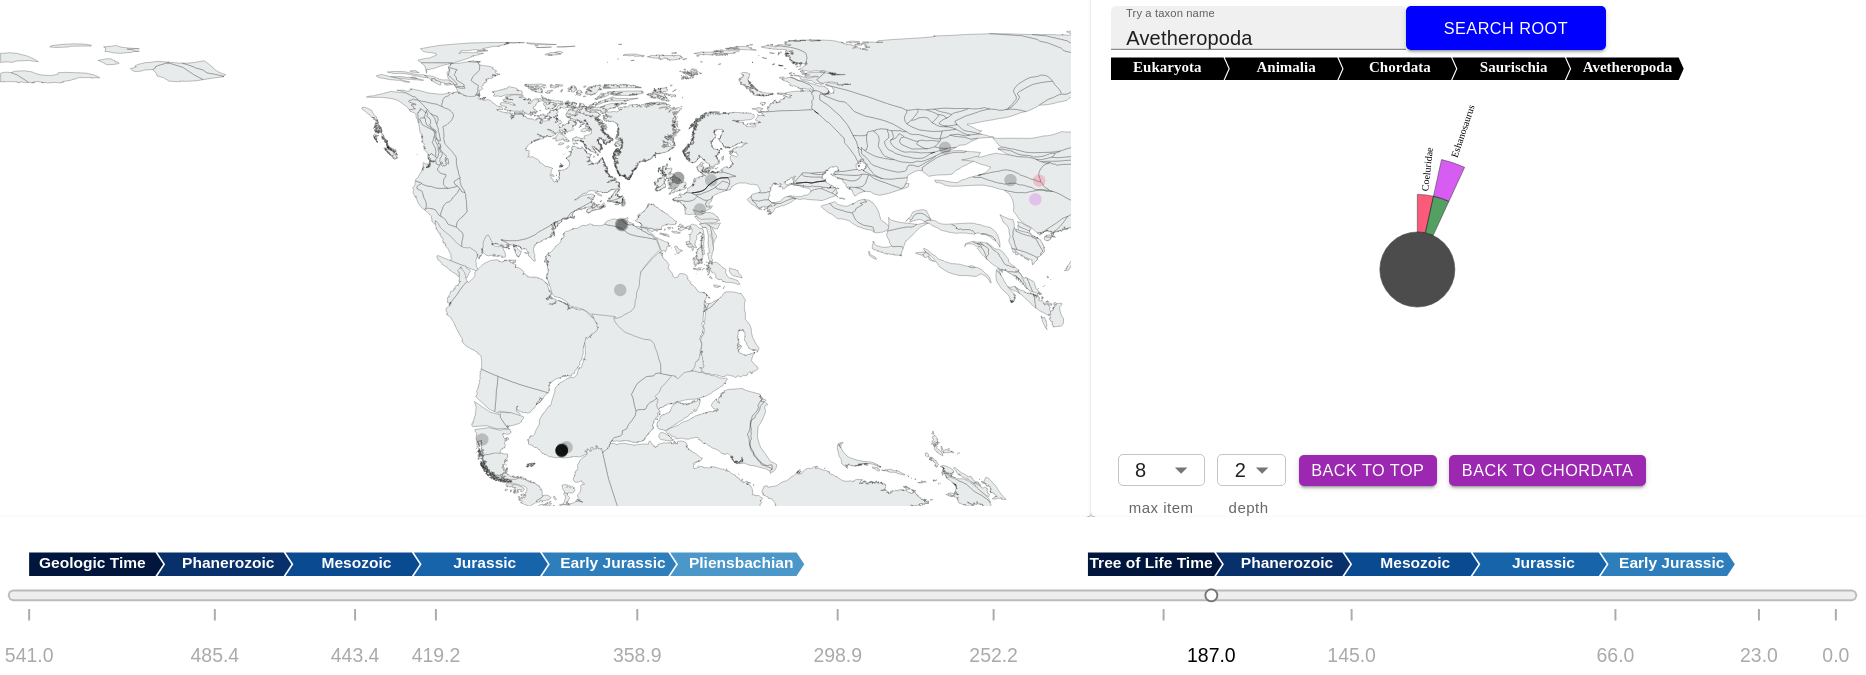
\includegraphics[width=0.7\textwidth]{figures/result/ave/EJu}\label{fig:EJu}} 
	\hfill
	\subfigure[Avetheropoda during Middle Jurassic. ]{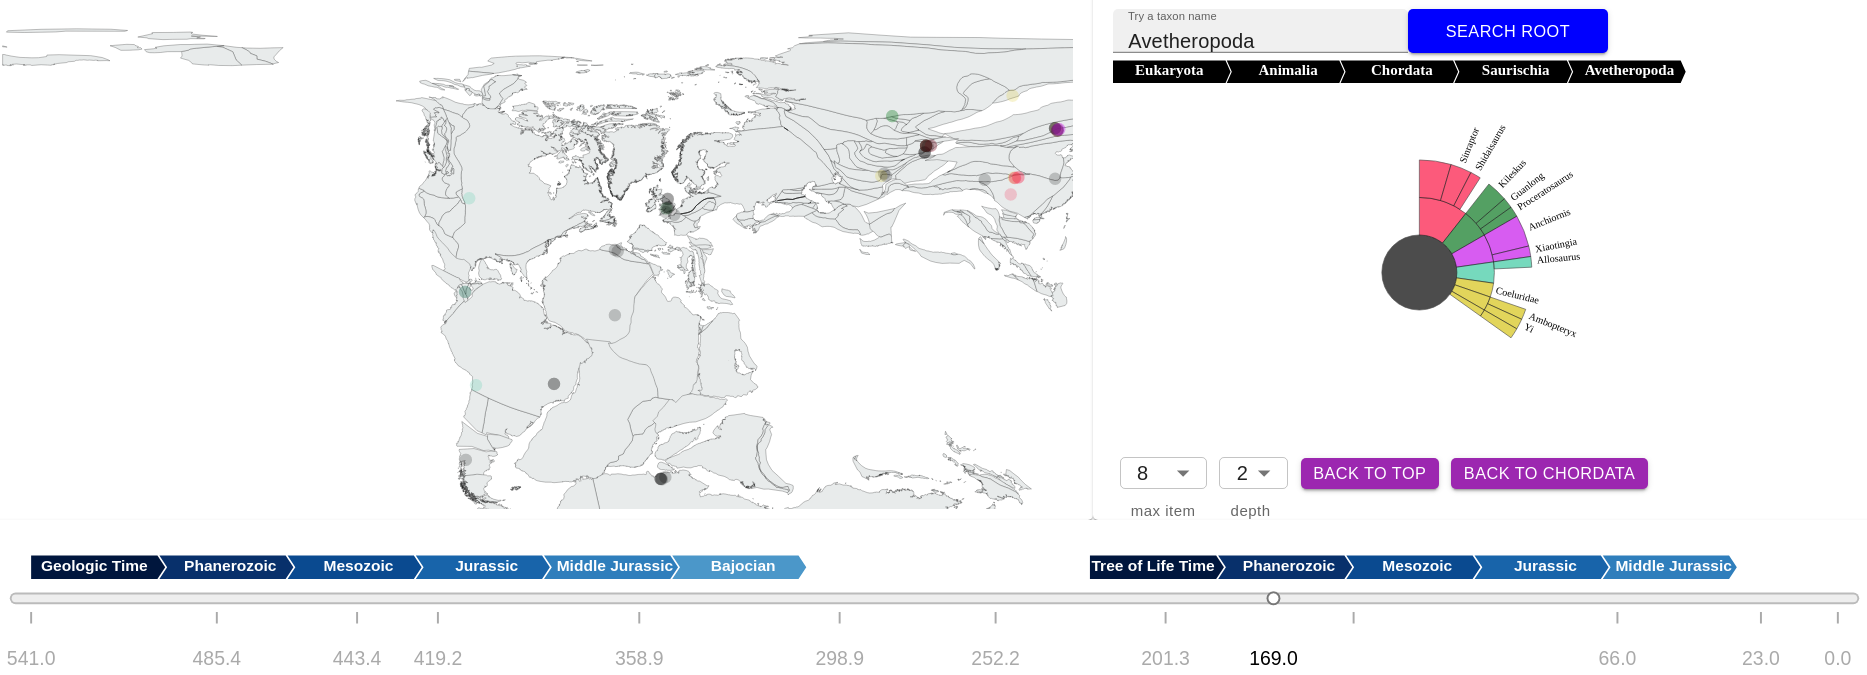
\includegraphics[width=0.7\textwidth]{figures/result/ave/MJu}\label{fig:MJu}} 
	\hfill
	\subfigure[Avetheropoda during Late Jurassic. ]{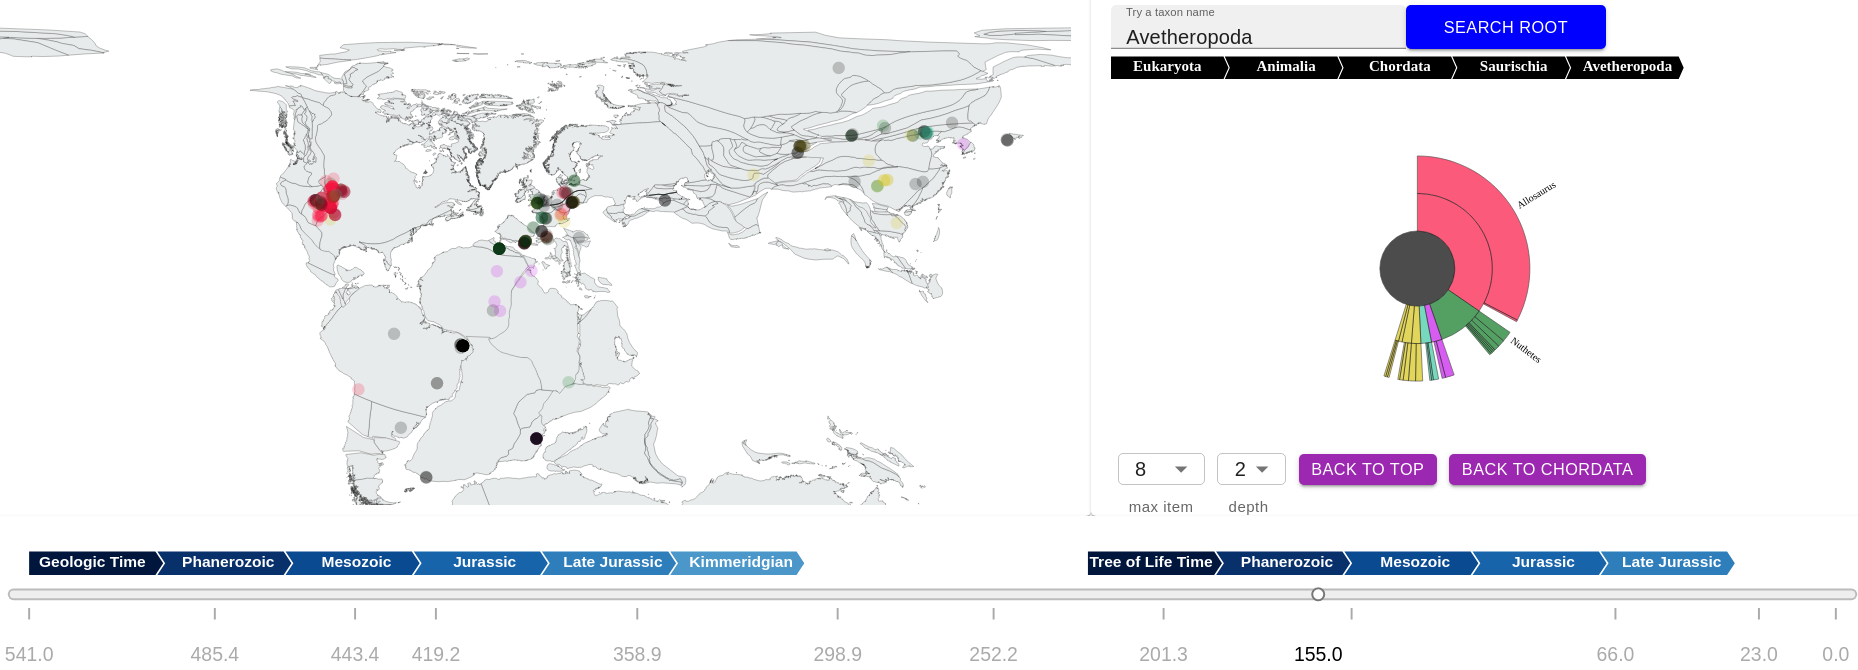
\includegraphics[width=0.7\textwidth]{figures/result/ave/LJu}\label{fig:LJu}} 
	\hfill
	\subfigure[Allosaurus dominates the Avetheropoda during Late Jurassic. ]{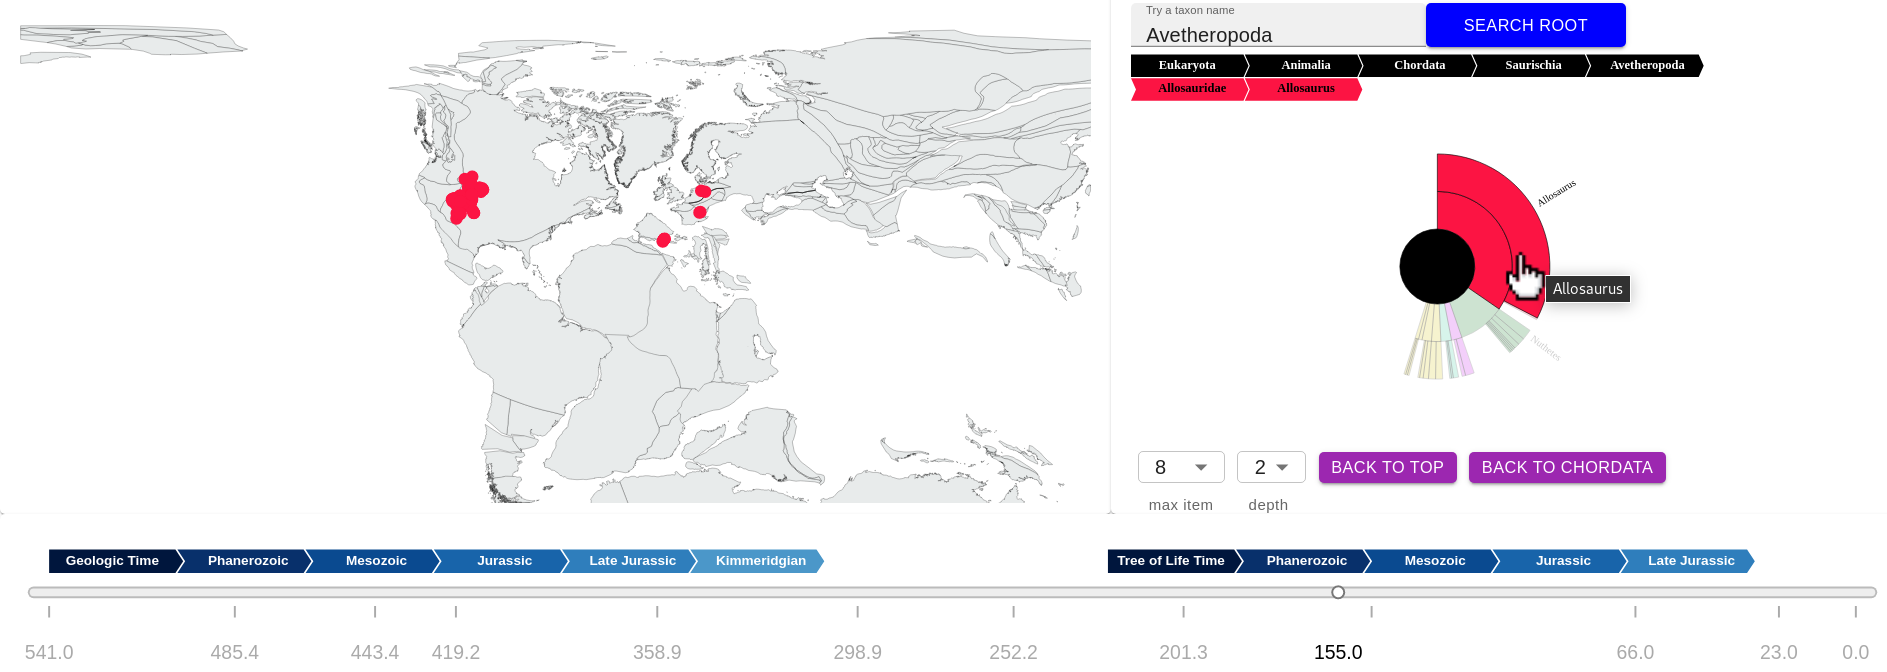
\includegraphics[width=0.7\textwidth]{figures/result/ave/LJu_dominant}\label{fig:LJu_dominant}} 
	
	
	\caption{The tree of life and fossil locations of Avetheropoda throughout Jurassic. The tree is directed to be under "Avetheropoda" while the time period moves forward, which can be seen in the time indicator in blue below the tree graph and the time value in the scroll bar at the bottom. The time table view is omitted for simplicity.}
	\label{fig:dinosaur_ju}
\end{figure}
\begin{figure}[h]
	\centering
	\subfigure[Avetheropoda during Early Cretaceous. ]{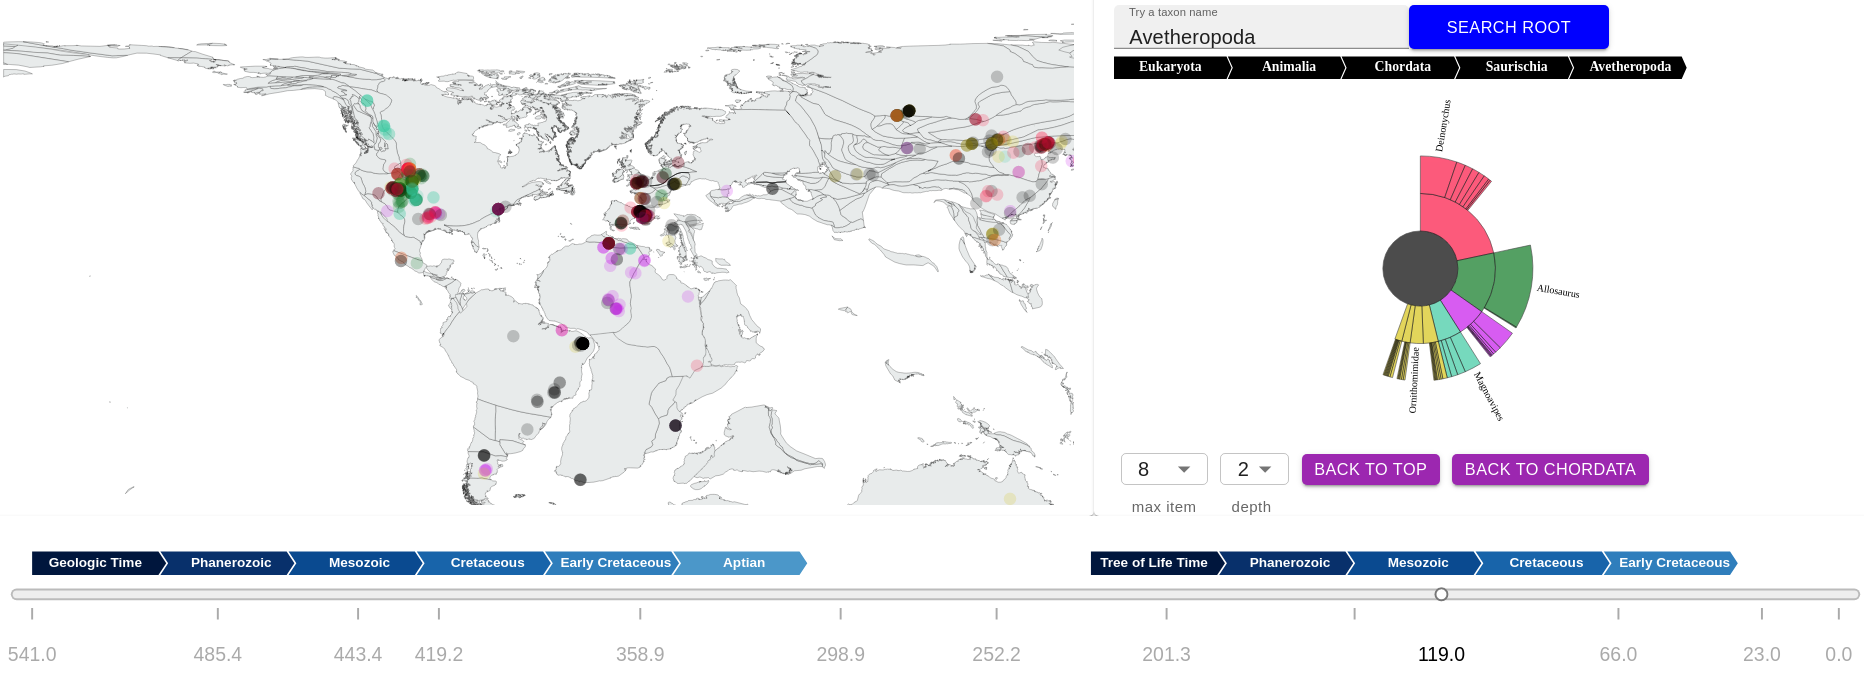
\includegraphics[width=0.7\textwidth]{figures/result/ave/ECre}\label{fig:ECre}}
	\hfill
	\subfigure[Avetheropoda during Late Cretaceous. The arrow is highlighting the genus Tyrannosaurus. ]{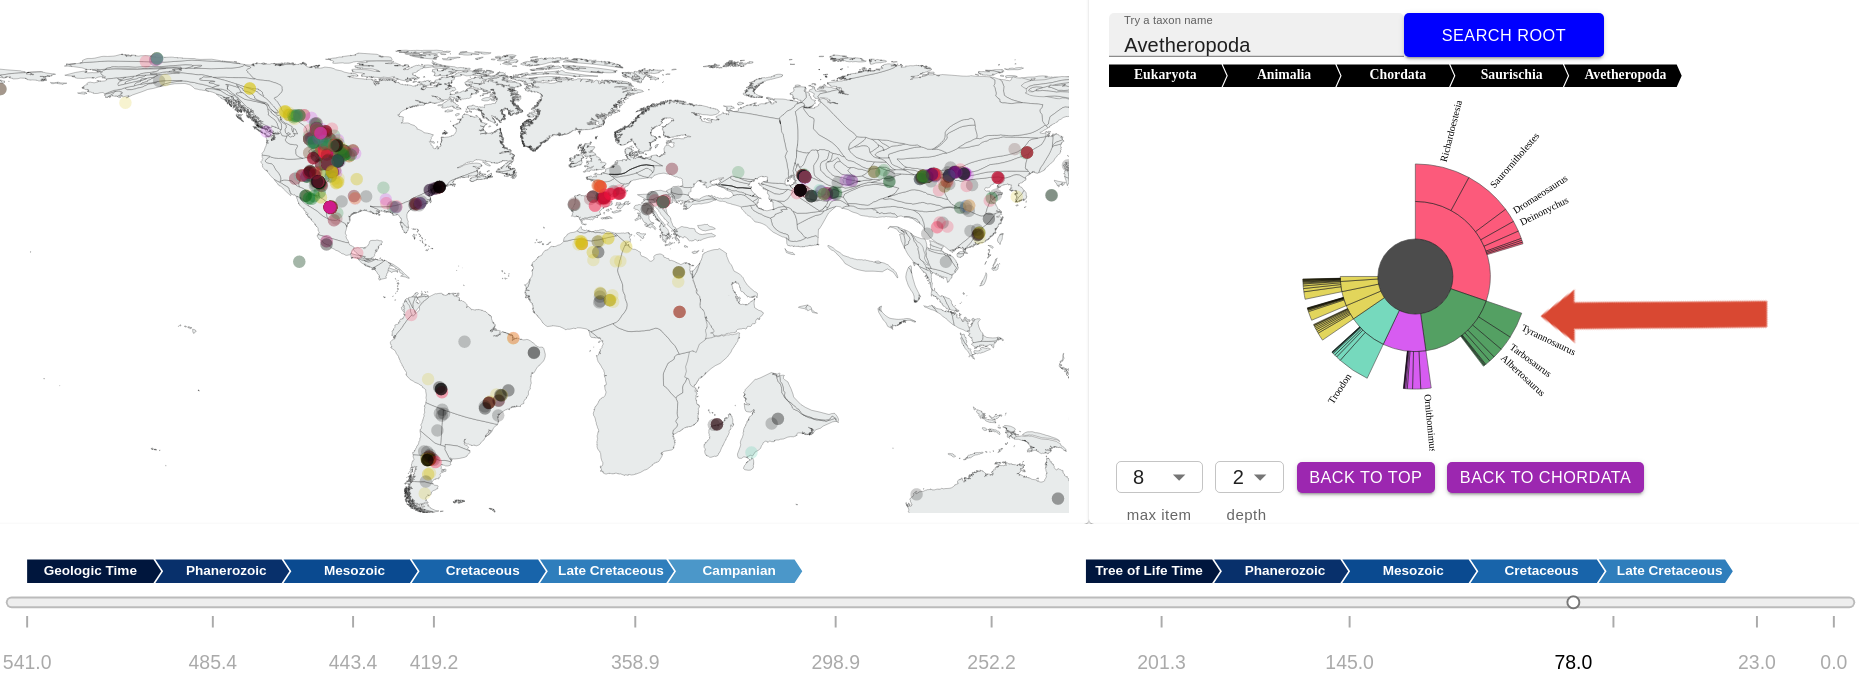
\includegraphics[width=0.7\textwidth]{figures/result/ave/LCre}\label{fig:LCre}}
	\hfill
	\subfigure[Avetheropoda during Danian, the first Age after Cretaceous. The arrow is highlighting the genus Tyrannosaurus. ]{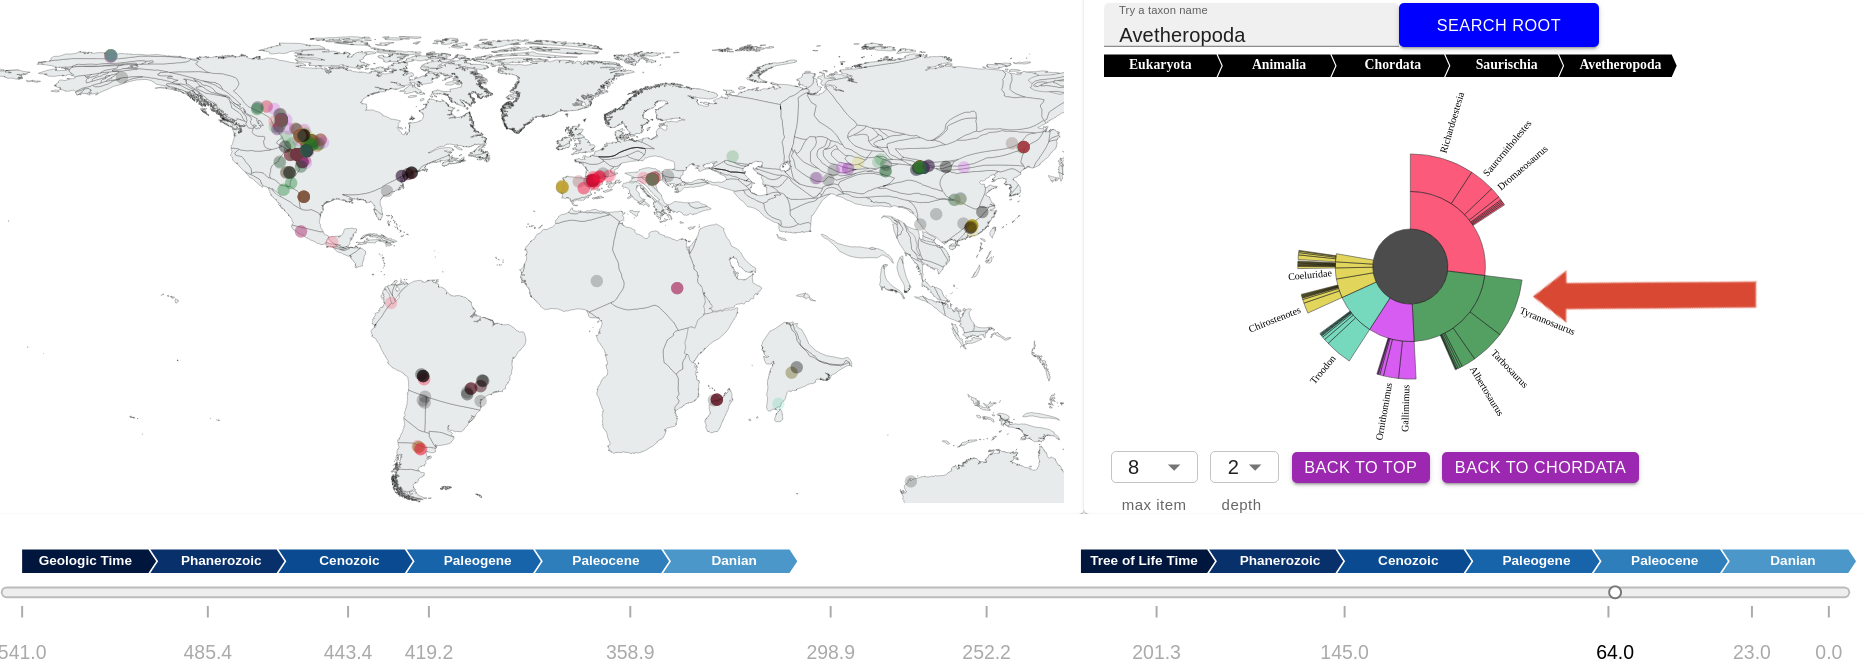
\includegraphics[width=0.7\textwidth]{figures/result/ave/before_disappear}\label{fig:before_disappear}}
	\subfigure[Avetheropoda during Selandian, the Age after Danian. The mouse is hovering on the only fossil found during this period.  ]{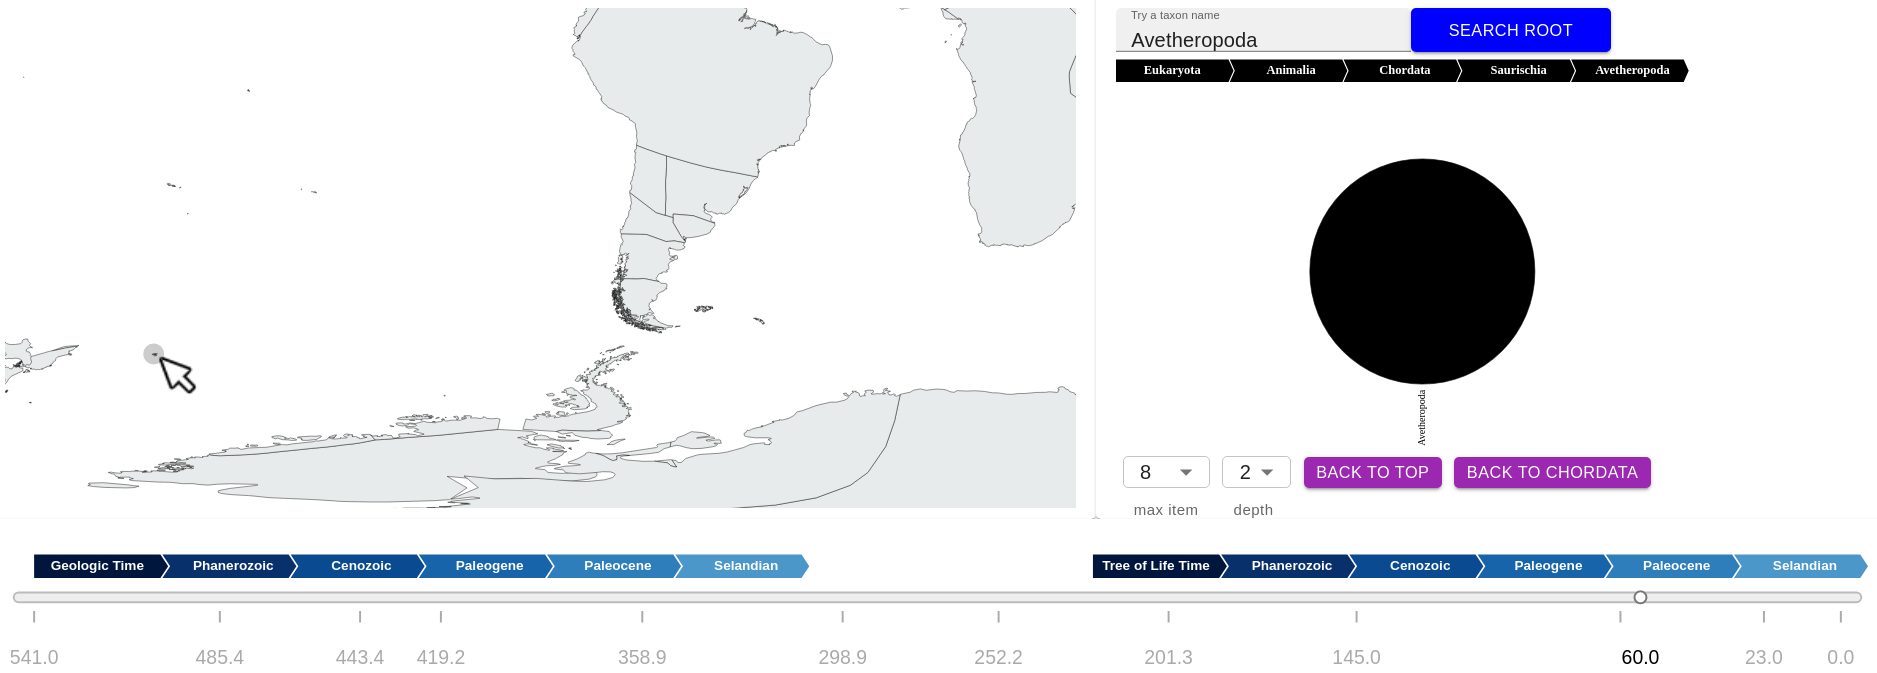
\includegraphics[width=0.7\textwidth]{figures/result/ave/disappear}\label{fig:disappear}}
	
	\caption{The tree of life and fossil locations of Avetheropoda throughout Cretaceous and shortly after. The time table view is omitted for simplicity.}
	\label{fig:dinosaur_cre}
\end{figure}
\begin{figure}[h]
	\centering
	\subfigure[Spatial distribution of Permian Dictoyopteridiales fossils at 276 million years ago, \emph{i.e.}, during their life time. ]{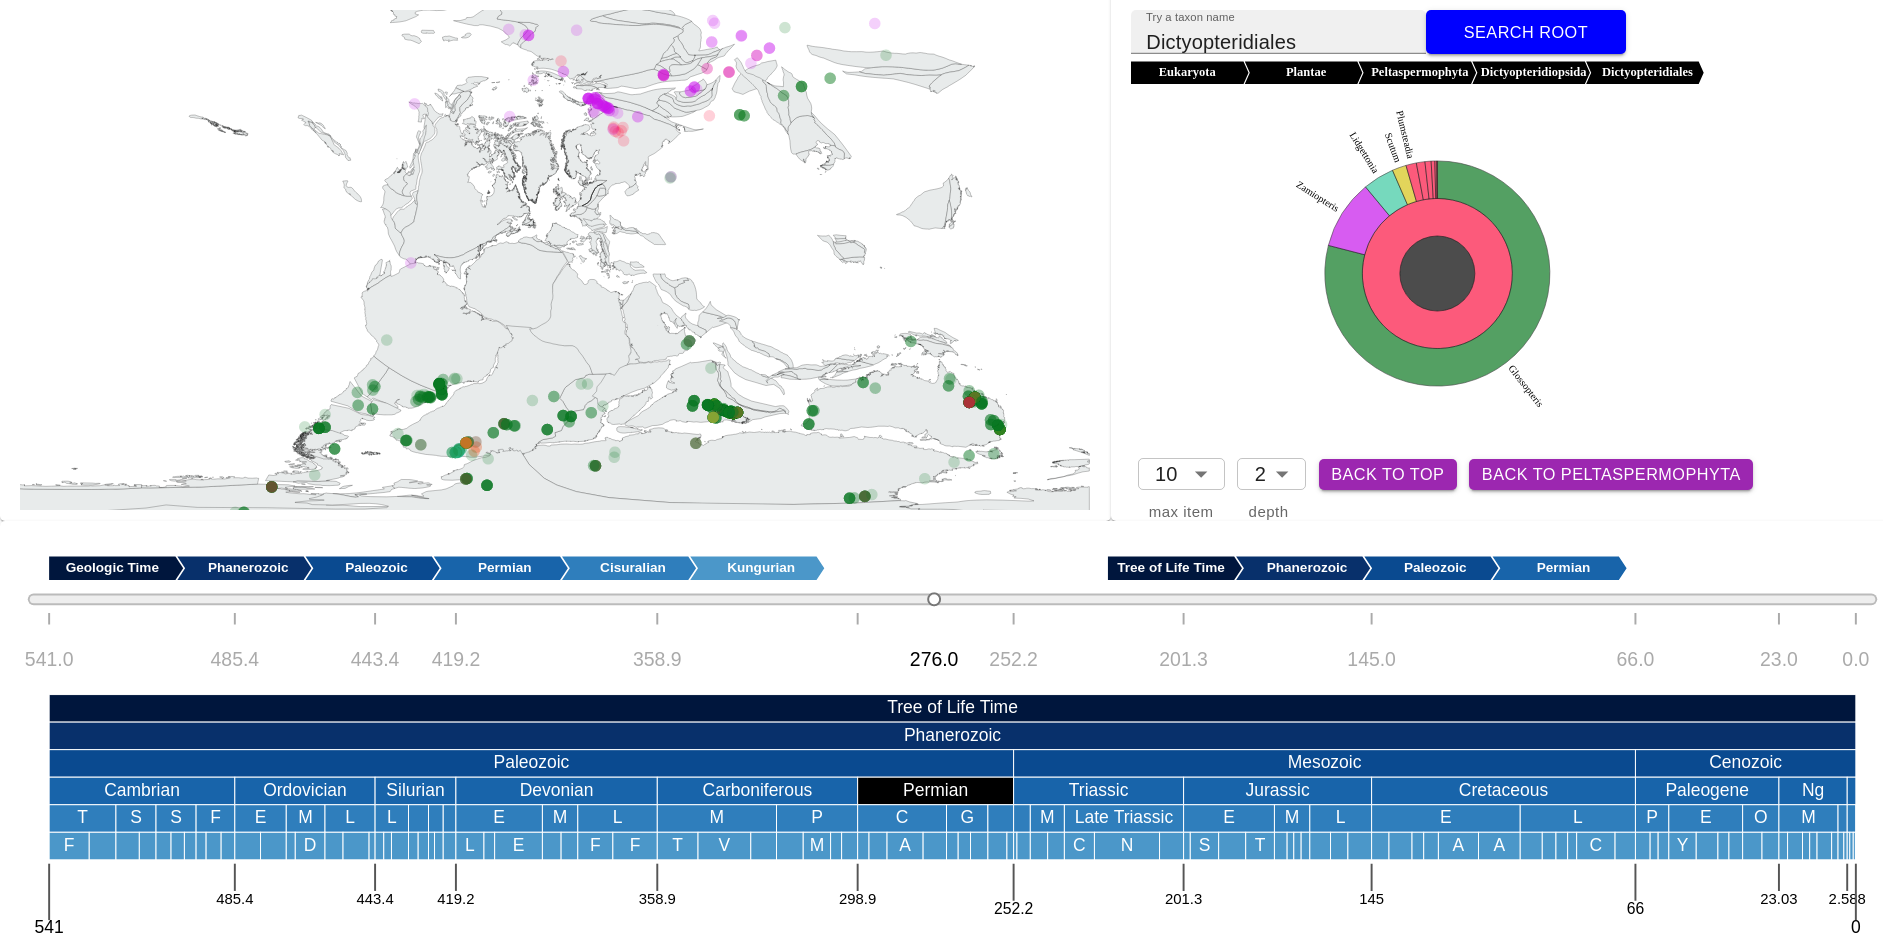
\includegraphics[width=0.5\textwidth]{figures/result/plant/permian}\label{fig:permian}} 
	\hfill
	\subfigure[Spatial distribution of the same fossils at 178 million years ago, \emph{i.e.}, around 100 million years since their death. ]{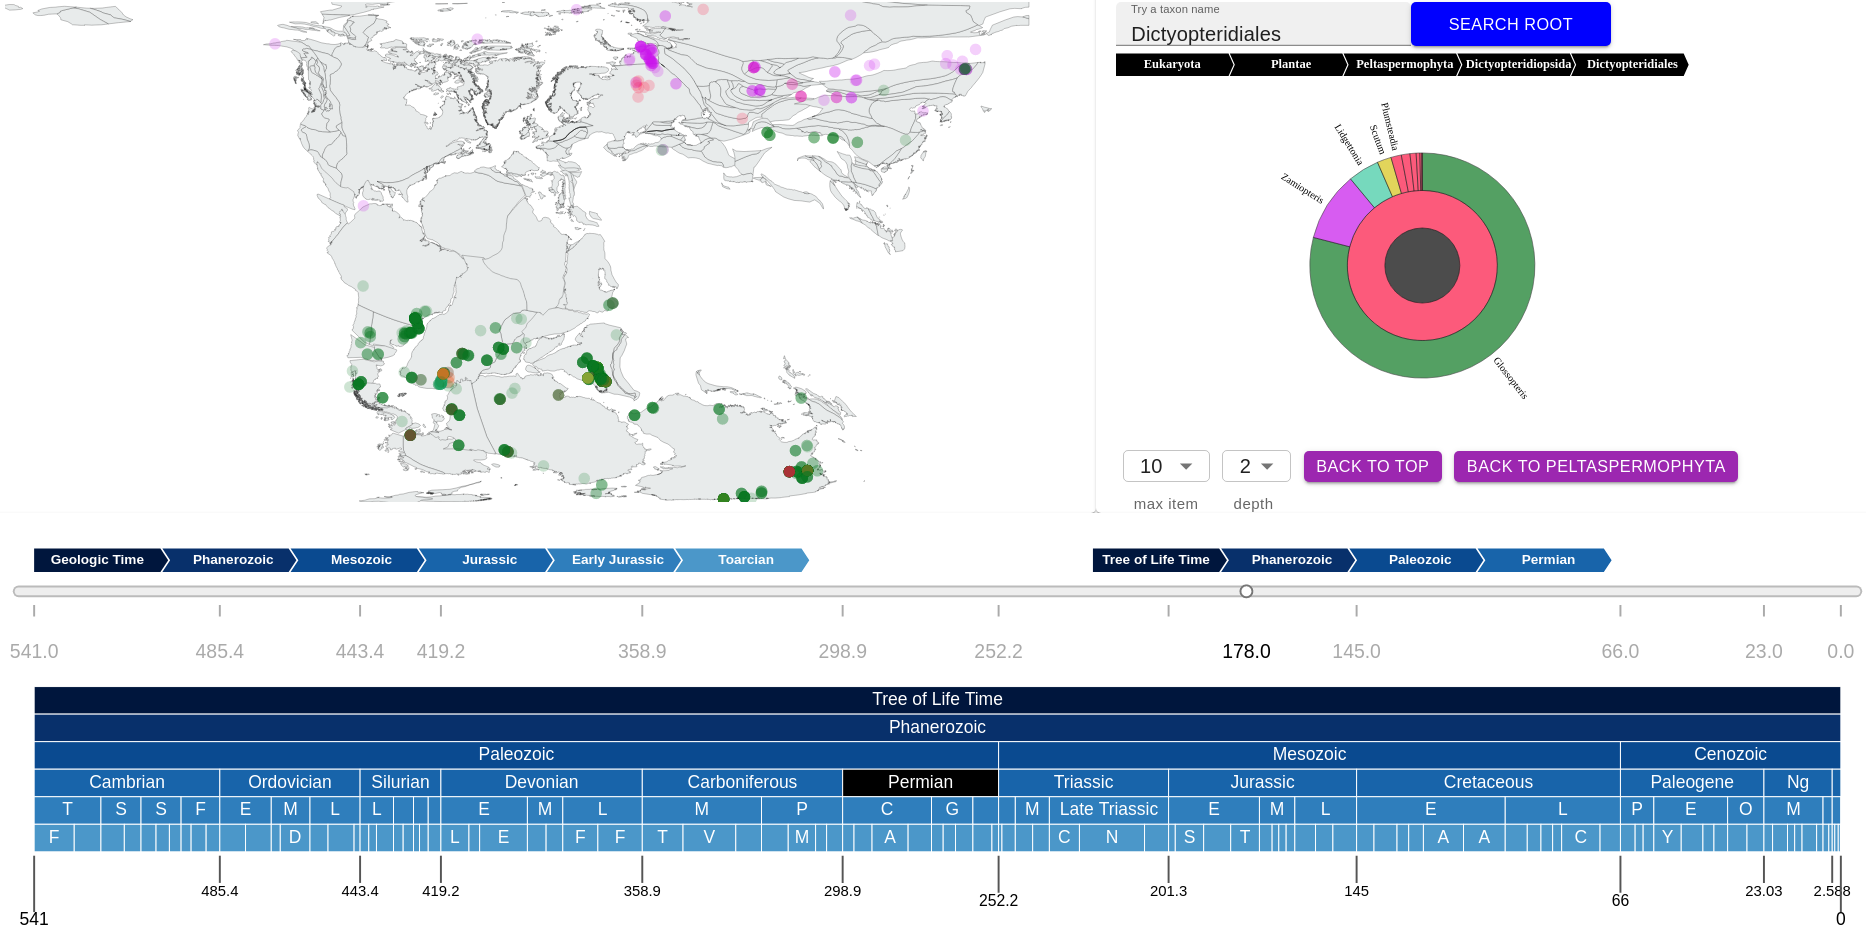
\includegraphics[width=0.5\textwidth]{figures/result/plant/jurassic}\label{fig:jurassic}} 
	\hfill
	\subfigure[Spatial distribution of the same fossils at 78 million years ago, \emph{i.e.}, around 200 million years since their death.. ]{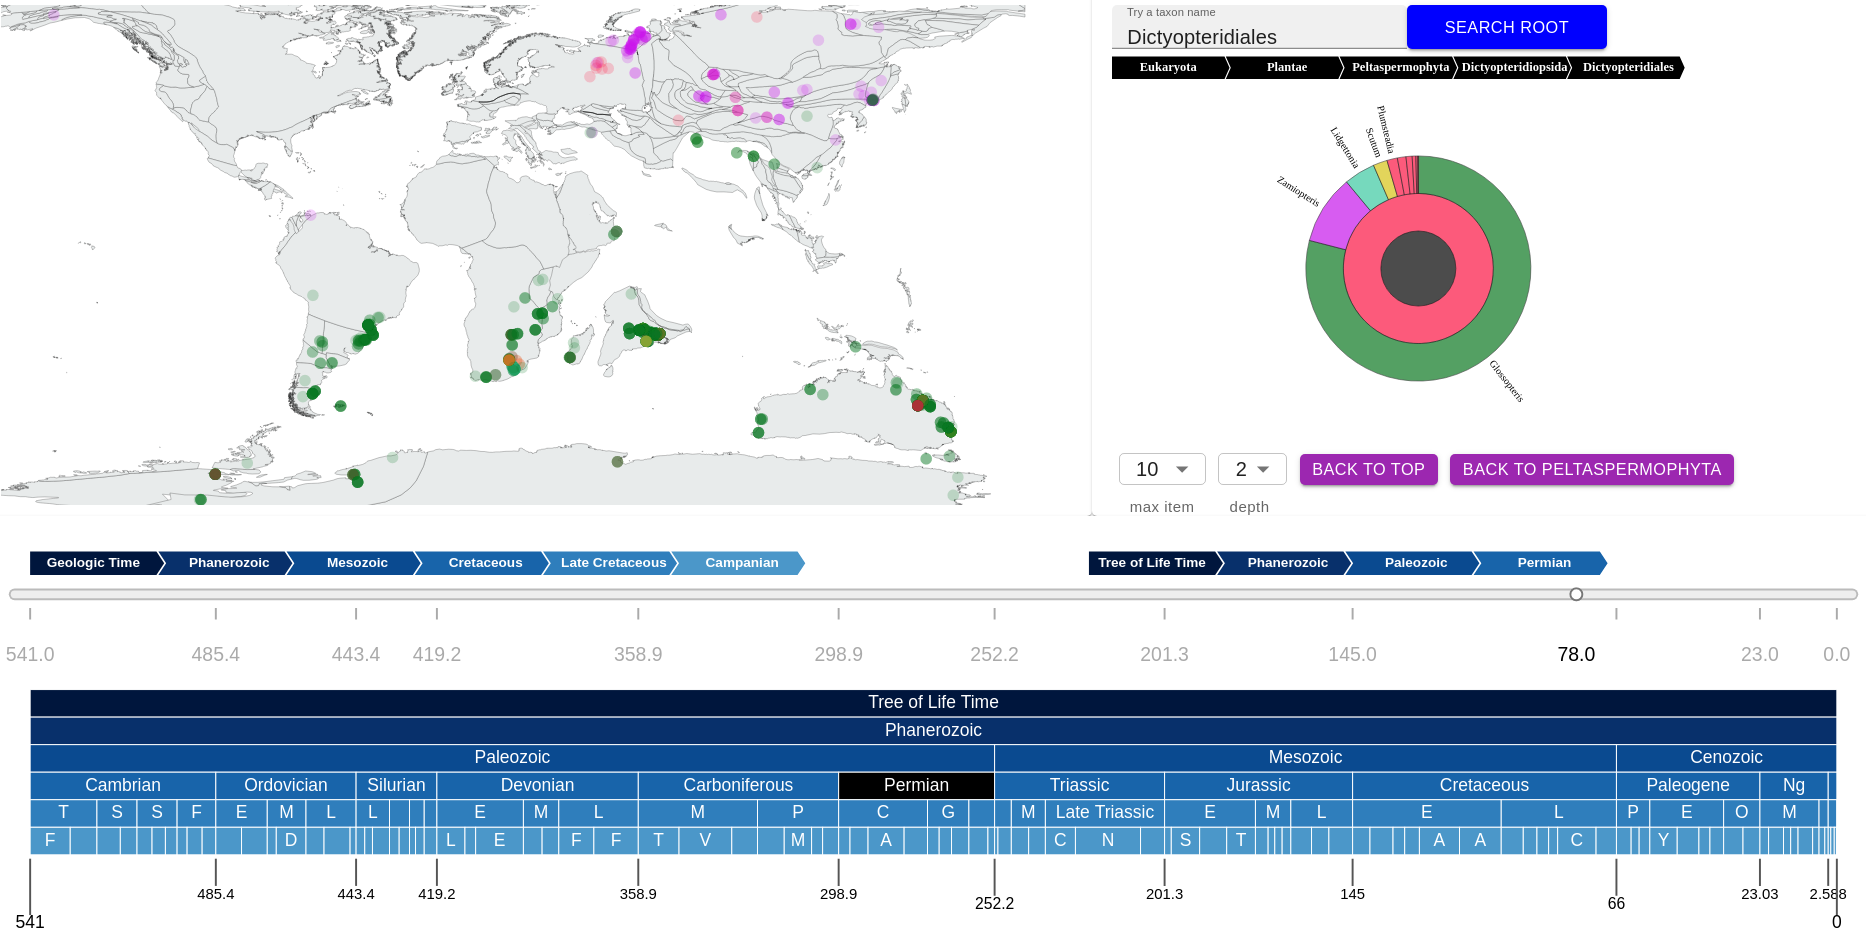
\includegraphics[width=0.5\textwidth]{figures/result/plant/cretaceous}\label{fig:cretaceous}} 
	\hfill
	\subfigure[Spatial distribution of the same fossils during modern days. ]{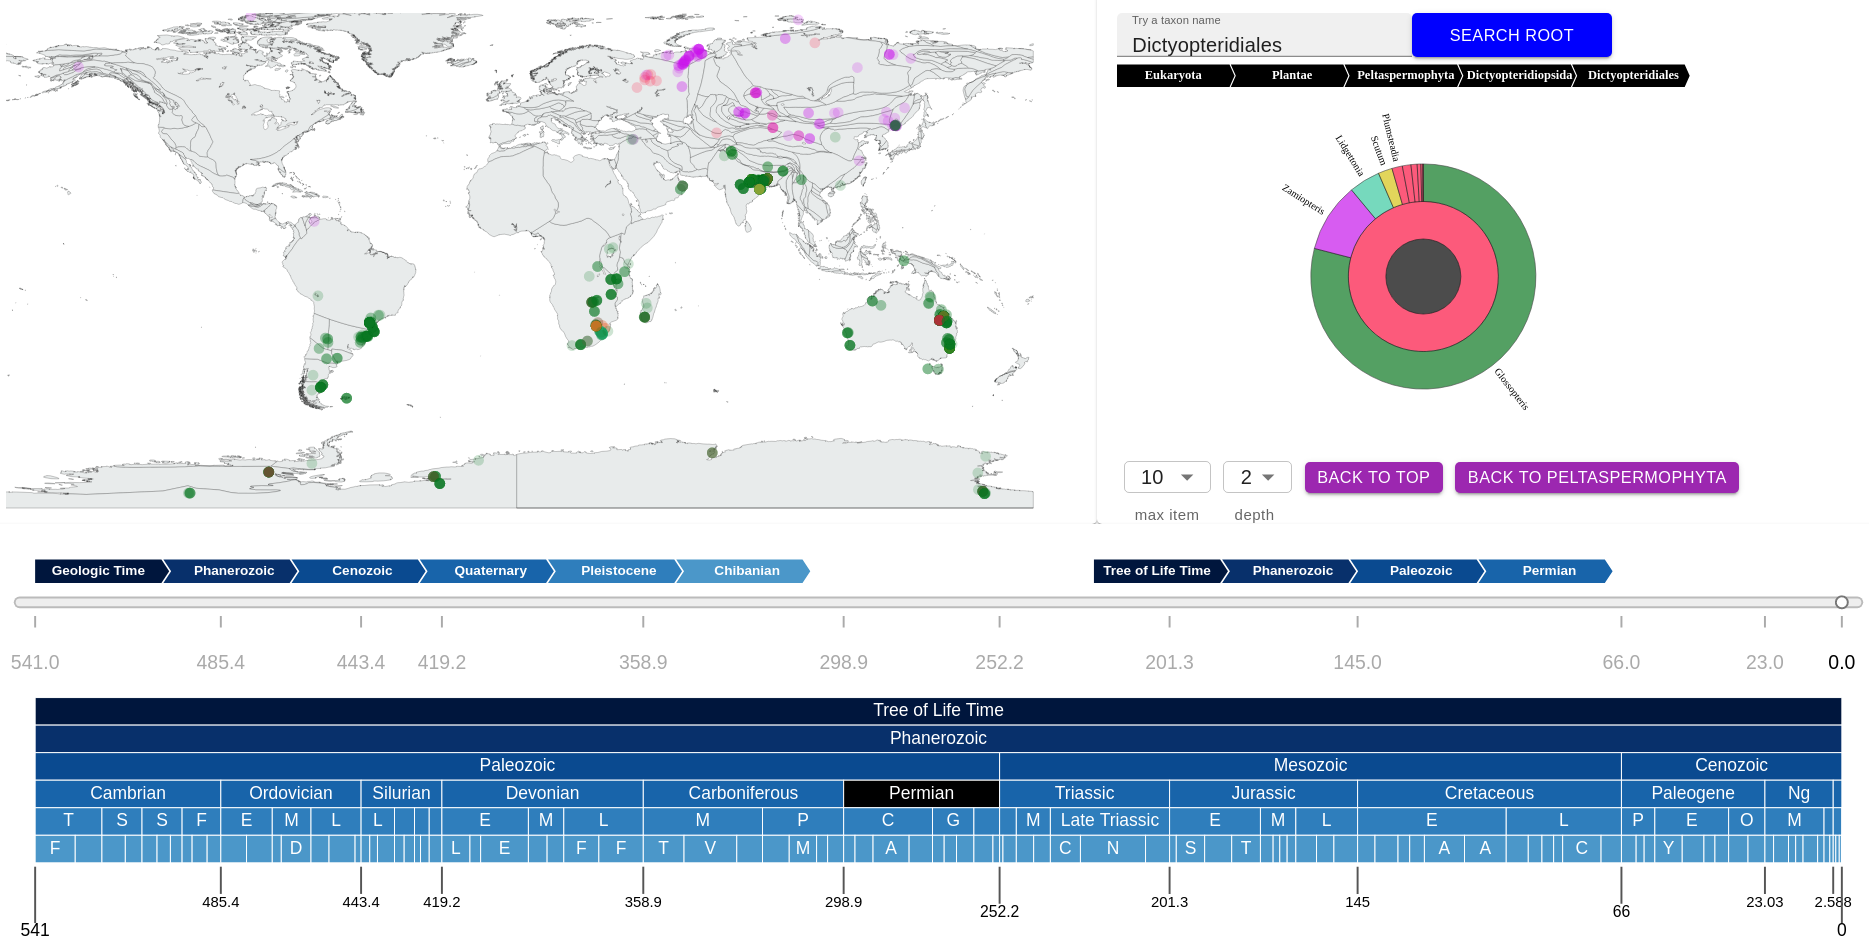
\includegraphics[width=0.5\textwidth]{figures/result/plant/modern}\label{fig:modern}} 
	
	\caption{The location change of Dictoyopteridiales fossils existed during Permian. The geological locations of the same fossils are tracked through time at an interval of 100 million years, in order to view how fossils move along with continental drift. It is easy to notice that green-marked fossils (under the genus of Glossopteris) inhabited together during their lifetime, however, their fossil locations separated in more recent times as a result of the tectonic shift.}
	\label{fig:plant}
\end{figure}
%=====================================================================
\chapter{Conclusion} \label{chp:conclusion}
%=====================================================================
Numerous visualizations on both the tree of life and Earth geology over time have been produced, as mentioned in chapter \ref{chp:related_work}. However, there still lacks a visualization that smoothly bridges data in both areas, while giving viewers the flexibility to explore how different forms of life lived in their environments at ancient times. Therefore, the primary contribution of this project is to provide such a visualization, which to our knowledge, is the first of its kind. \\

The current project purposes a way to construct a tree of life from names on taxonomic ranks, by exploiting the parent-child relationship in those ranks. We generate a \emph{path\_from\_root} value for each fossil, which.is used as a unique identifier of a tree node. Since all ancestors are naturally encoded in the path, we can conveniently locate a node's position in the complete tree, or search a node's subtree. We have also designed a data schema that is suitable for the needs of the visualization. In short, tree data is linked to the attached fossils via the \emph{path\_from\_root} value, and fossil data is linked to their location data via fossil IDs. \\

Finally, the visualization allows users to explore biodiversity in the following ways. Users can select a taxonomy and a time period of interest to view the tree of life under this taxonomy. In addition, the fossils classified under the taxonomy that existed during the selected time period are also shown on a world map at the ancient time point. All fossils attached to a particular node can be highlighted on the map when hovering on the node, and hovering on a fossil point highlights its taxonomic information on the tree. This interaction between map and tree components enables users to be aware of both the spatial distribution of a certain node's fossils and what taxonomy a certain fossil belongs to. It is possible to customize the tree of life by setting its depth and breadth. Users can also freely navigate through the tree by clicking on a node of interest in the tree graph or clicking on an ancestor shown above the tree graph. A scroll bar for time enables tracing of how plate motion brings fossils to different locations over millions of years. \\

To summarize, this project suggests a method to process, store and visualize taxonomic and geological data, leading to a novel and dynamic visualization of how Earth, the home to all life, has nourished a great diversity of organisms over the past millions of years.

\section{Limitations and future Work}
Currently, the tree of life is generated from the taxonomic information of the fossils. However, there exist several online taxonomy databases, such as Wikidata \cite{vrandevcic2014wikidata} and the NCBI taxonomy database \cite{federhen2012ncbi}, which contain more information on taxonomy (\emph{e.g.}, short introduction, pictures). Each node in the current tree of life can be associated with another database, such that users can be directed via an external link to some extra information on the taxonomy. In fact, a major effort has been put to organize the taxonomy of Wikidata into a tree of life. However, the attempt failed to associate fossils to nodes of the Wikidata tree, due to the serious inconsistencies in naming and parent-child relationships. For instance, the flowering plant is termed "Angiospermae" in fossil data but "Magnoliophyta" in Wikidata, and they also belong to different taxonomic ranks in the two datasets. As a result, simply linking by name matching could attach the fossils to a wrong node, or fail to attach the fossils to any node. Therefore, future work could focus on associating the current tree of life to an external database, with the help of domain knowledge in taxonomy.\\

Although the earliest fossil in the current dataset dates back to 1000 million years, and the start of the timescale is 541 million years ago, the earliest available map and fossil location reconstruction only begin at 410 million years ago, limited by the plate motion model. Future work can combine other models that simulate global plate motion earlier than 410 million years ago, such that fossils in time periods earlier than the current limit can be shown on the map. \\

It is also beneficial to further enrich the current visualization with other types of data. Special events that shaped the evolutionary path, such as the asteroid 66 million years ago that led to the fall of the dinosaurs, can be included by marking the timetable with texts. Temperature, oxygen level, and carbon dioxide level are also considered to be major environmental factors that dictate evolution \cite{butterfield2009oxygen, svenning2007ice}. Therefore, their values can be provided in an information panel in the map component that updates in response to the current time point of the map. 


%=====================================================================
\chapter*{Acknowledgements}
%=====================================================================
Most importantly, I would like to thank my direct supervisor Gaudenz Halter for his consistent guidance throughout my whole progress. His feedback has always helped to keep my work on the right track. I would also like to thank Prof. Dr. Renato
Pajarola for providing me the opportunity to write this thesis and begin my journey in data visualization. Lastly, I would like to appreciate the company of my girlfriend and my parents. Their mental support is essential to keep me motivated during my ups and downs.

\bibliographystyle{alpha}
\bibliography{references}

\listoffigures
\listoftables
%=====================================================================
\end{document}

